\subsection{Аналитическая геометрия}
	
	\subsubsection{Общие сведения об опросе}

	    Курс <<Аналитическая геометрия>> в целом получил положительные отзывы.
        
        Лекции Чубарова И.А. получили крайне положительные отзывы, однако есть ряд недостатков. Студенты отметили, что лекциям не хватило структурированности и было не слышно, что говорит лектор без использования микрофона. Совет студентов и аспирантов ФРКТ просит передать эти сведения лектору.

        Семинаристы Агаханова Я.С., Глухова Е.В., Чубаров И.А. получили крайне положительные оценки от респондентов. Совет студентов и аспирантов ФРКТ предлагает поощрить перечисленных преподавателей.

        Семинарист Петрович А.А. получила негативные отзывы. Респонденты отметили, что семинарист не разбирается в предмете и непонятно объясняет материал. Совет студентов и аспирантов ФРКТ рекомендует заменить этого семинариста.

	\subsubsection{Общий отзыв студентов о курсе}

		\begin{figure}[H]
			\centering
			\begin{subfigure}[b]{0.45\textwidth}
				\centering
				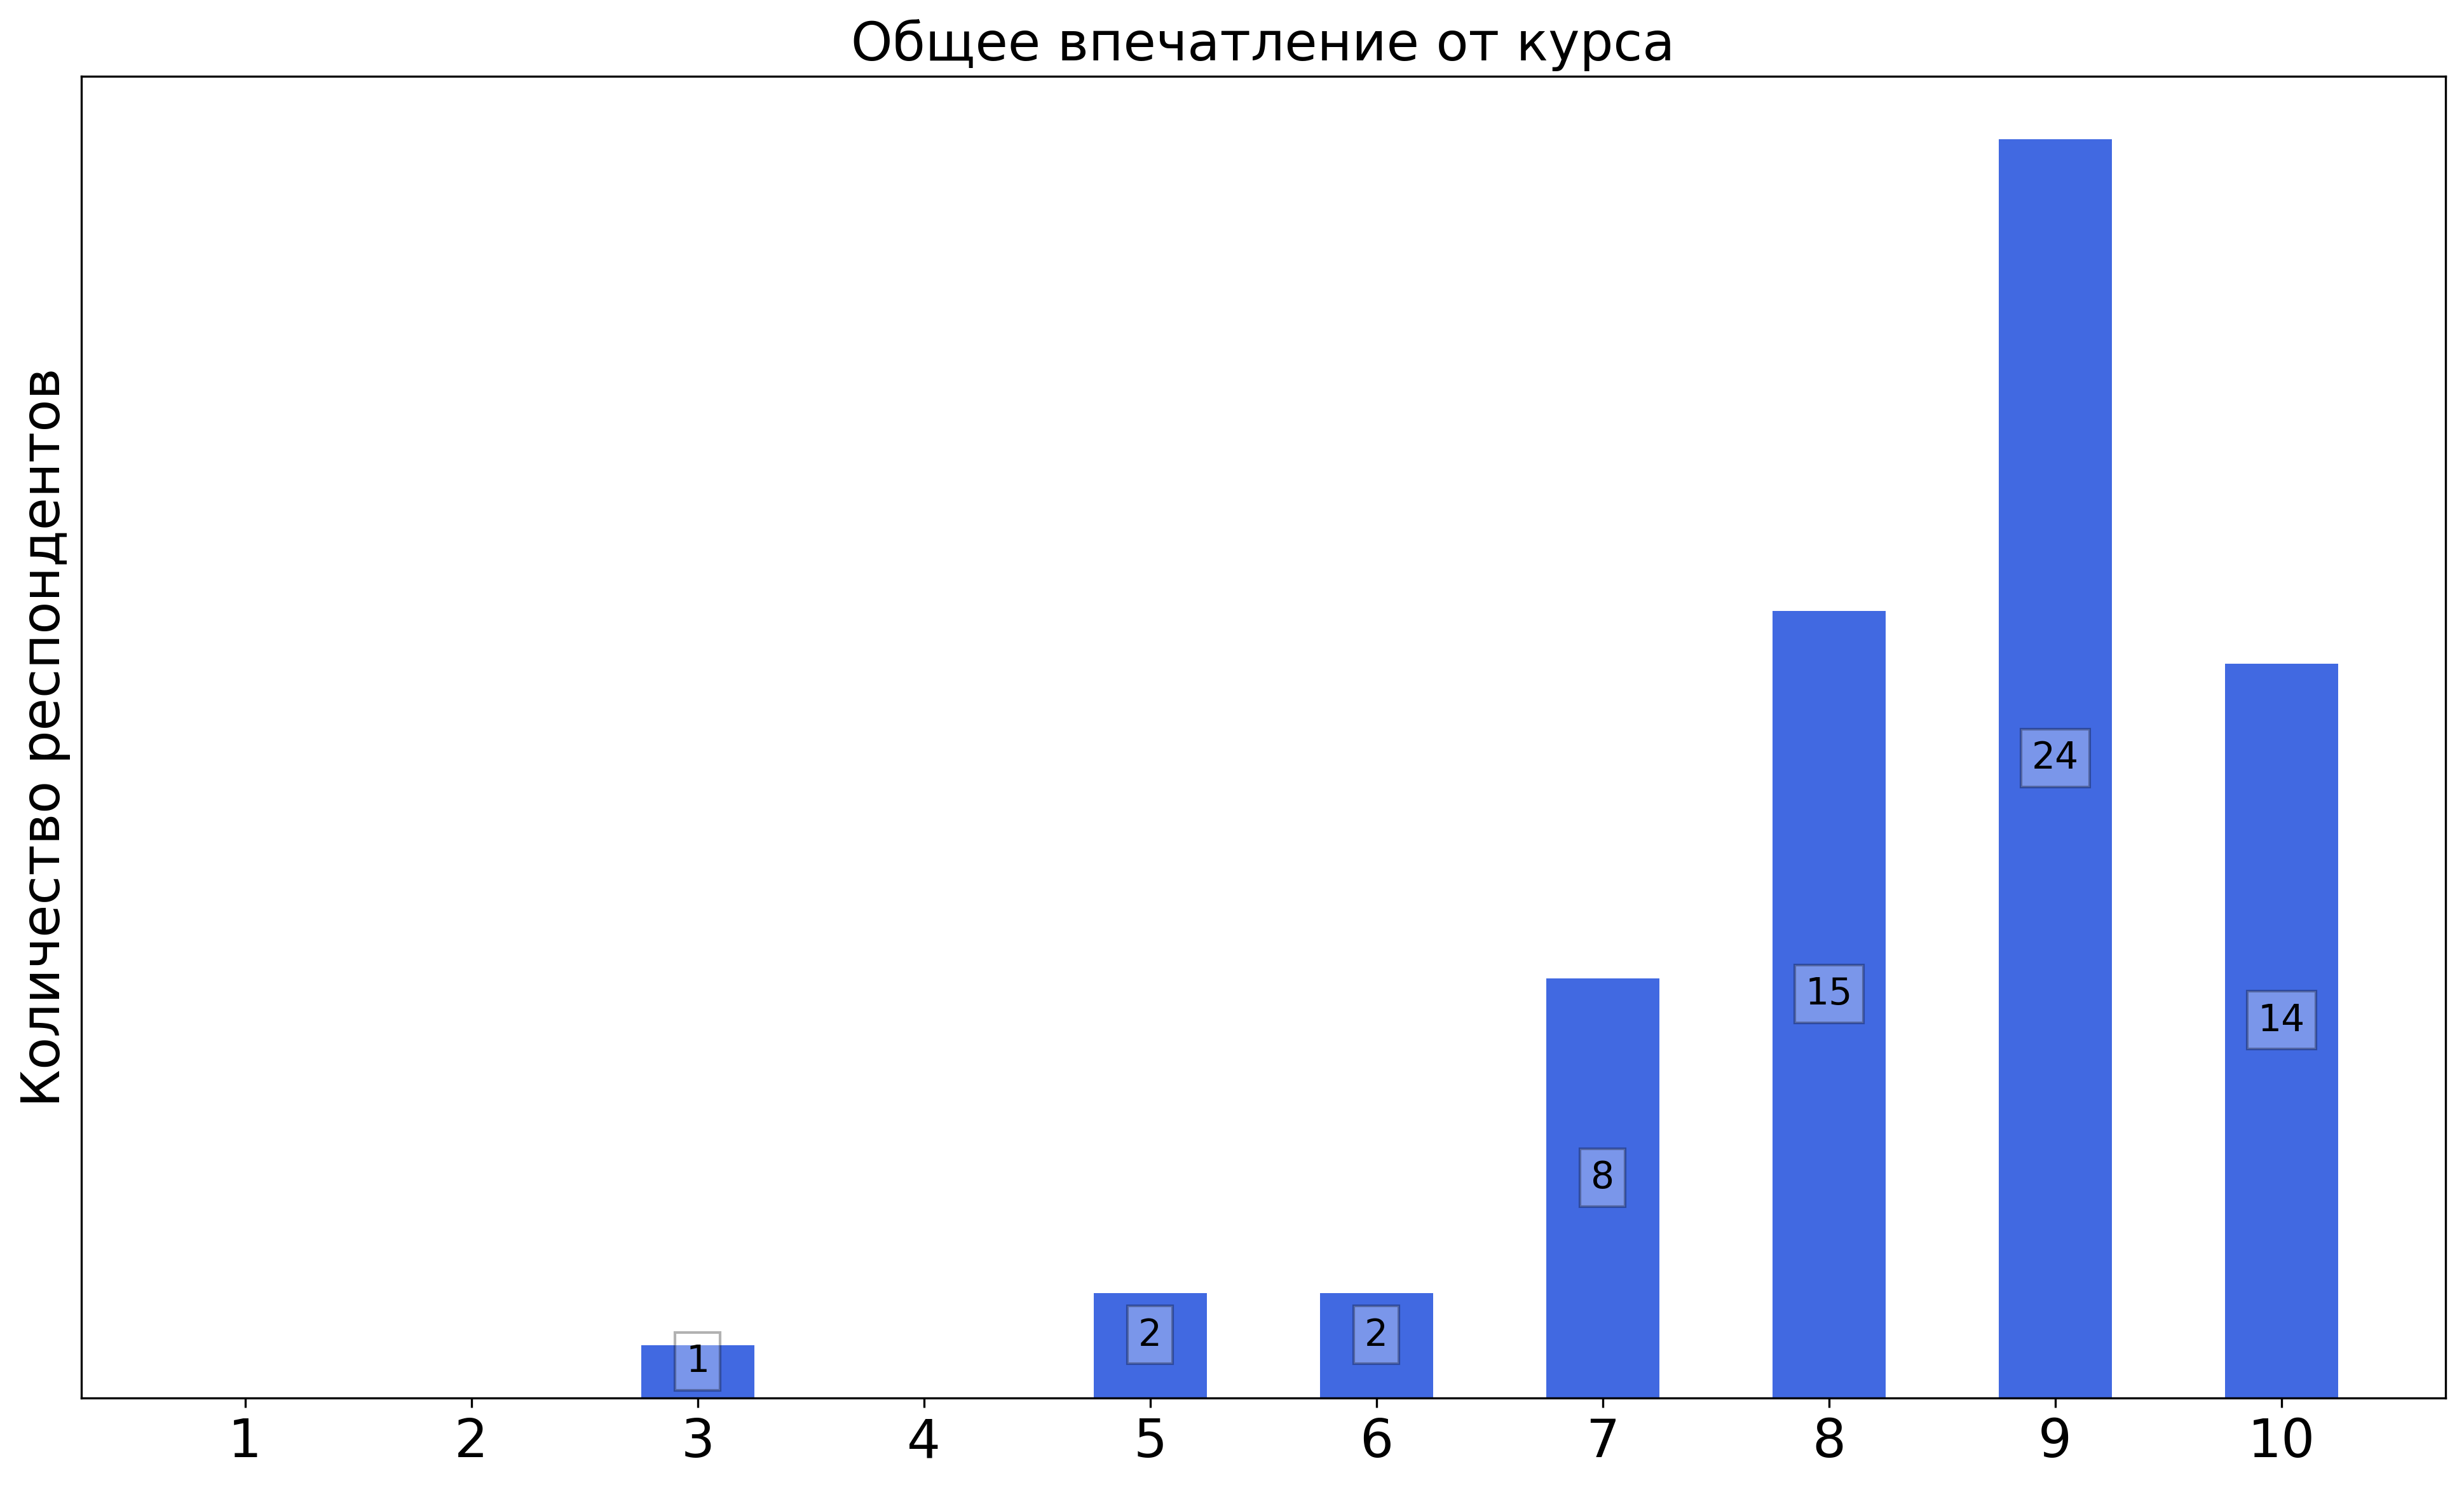
\includegraphics[width=\textwidth]{images/1 course/Аналитическая геометрия/general-0.png}
			\end{subfigure}
			\begin{subfigure}[b]{0.45\textwidth}
				\centering
				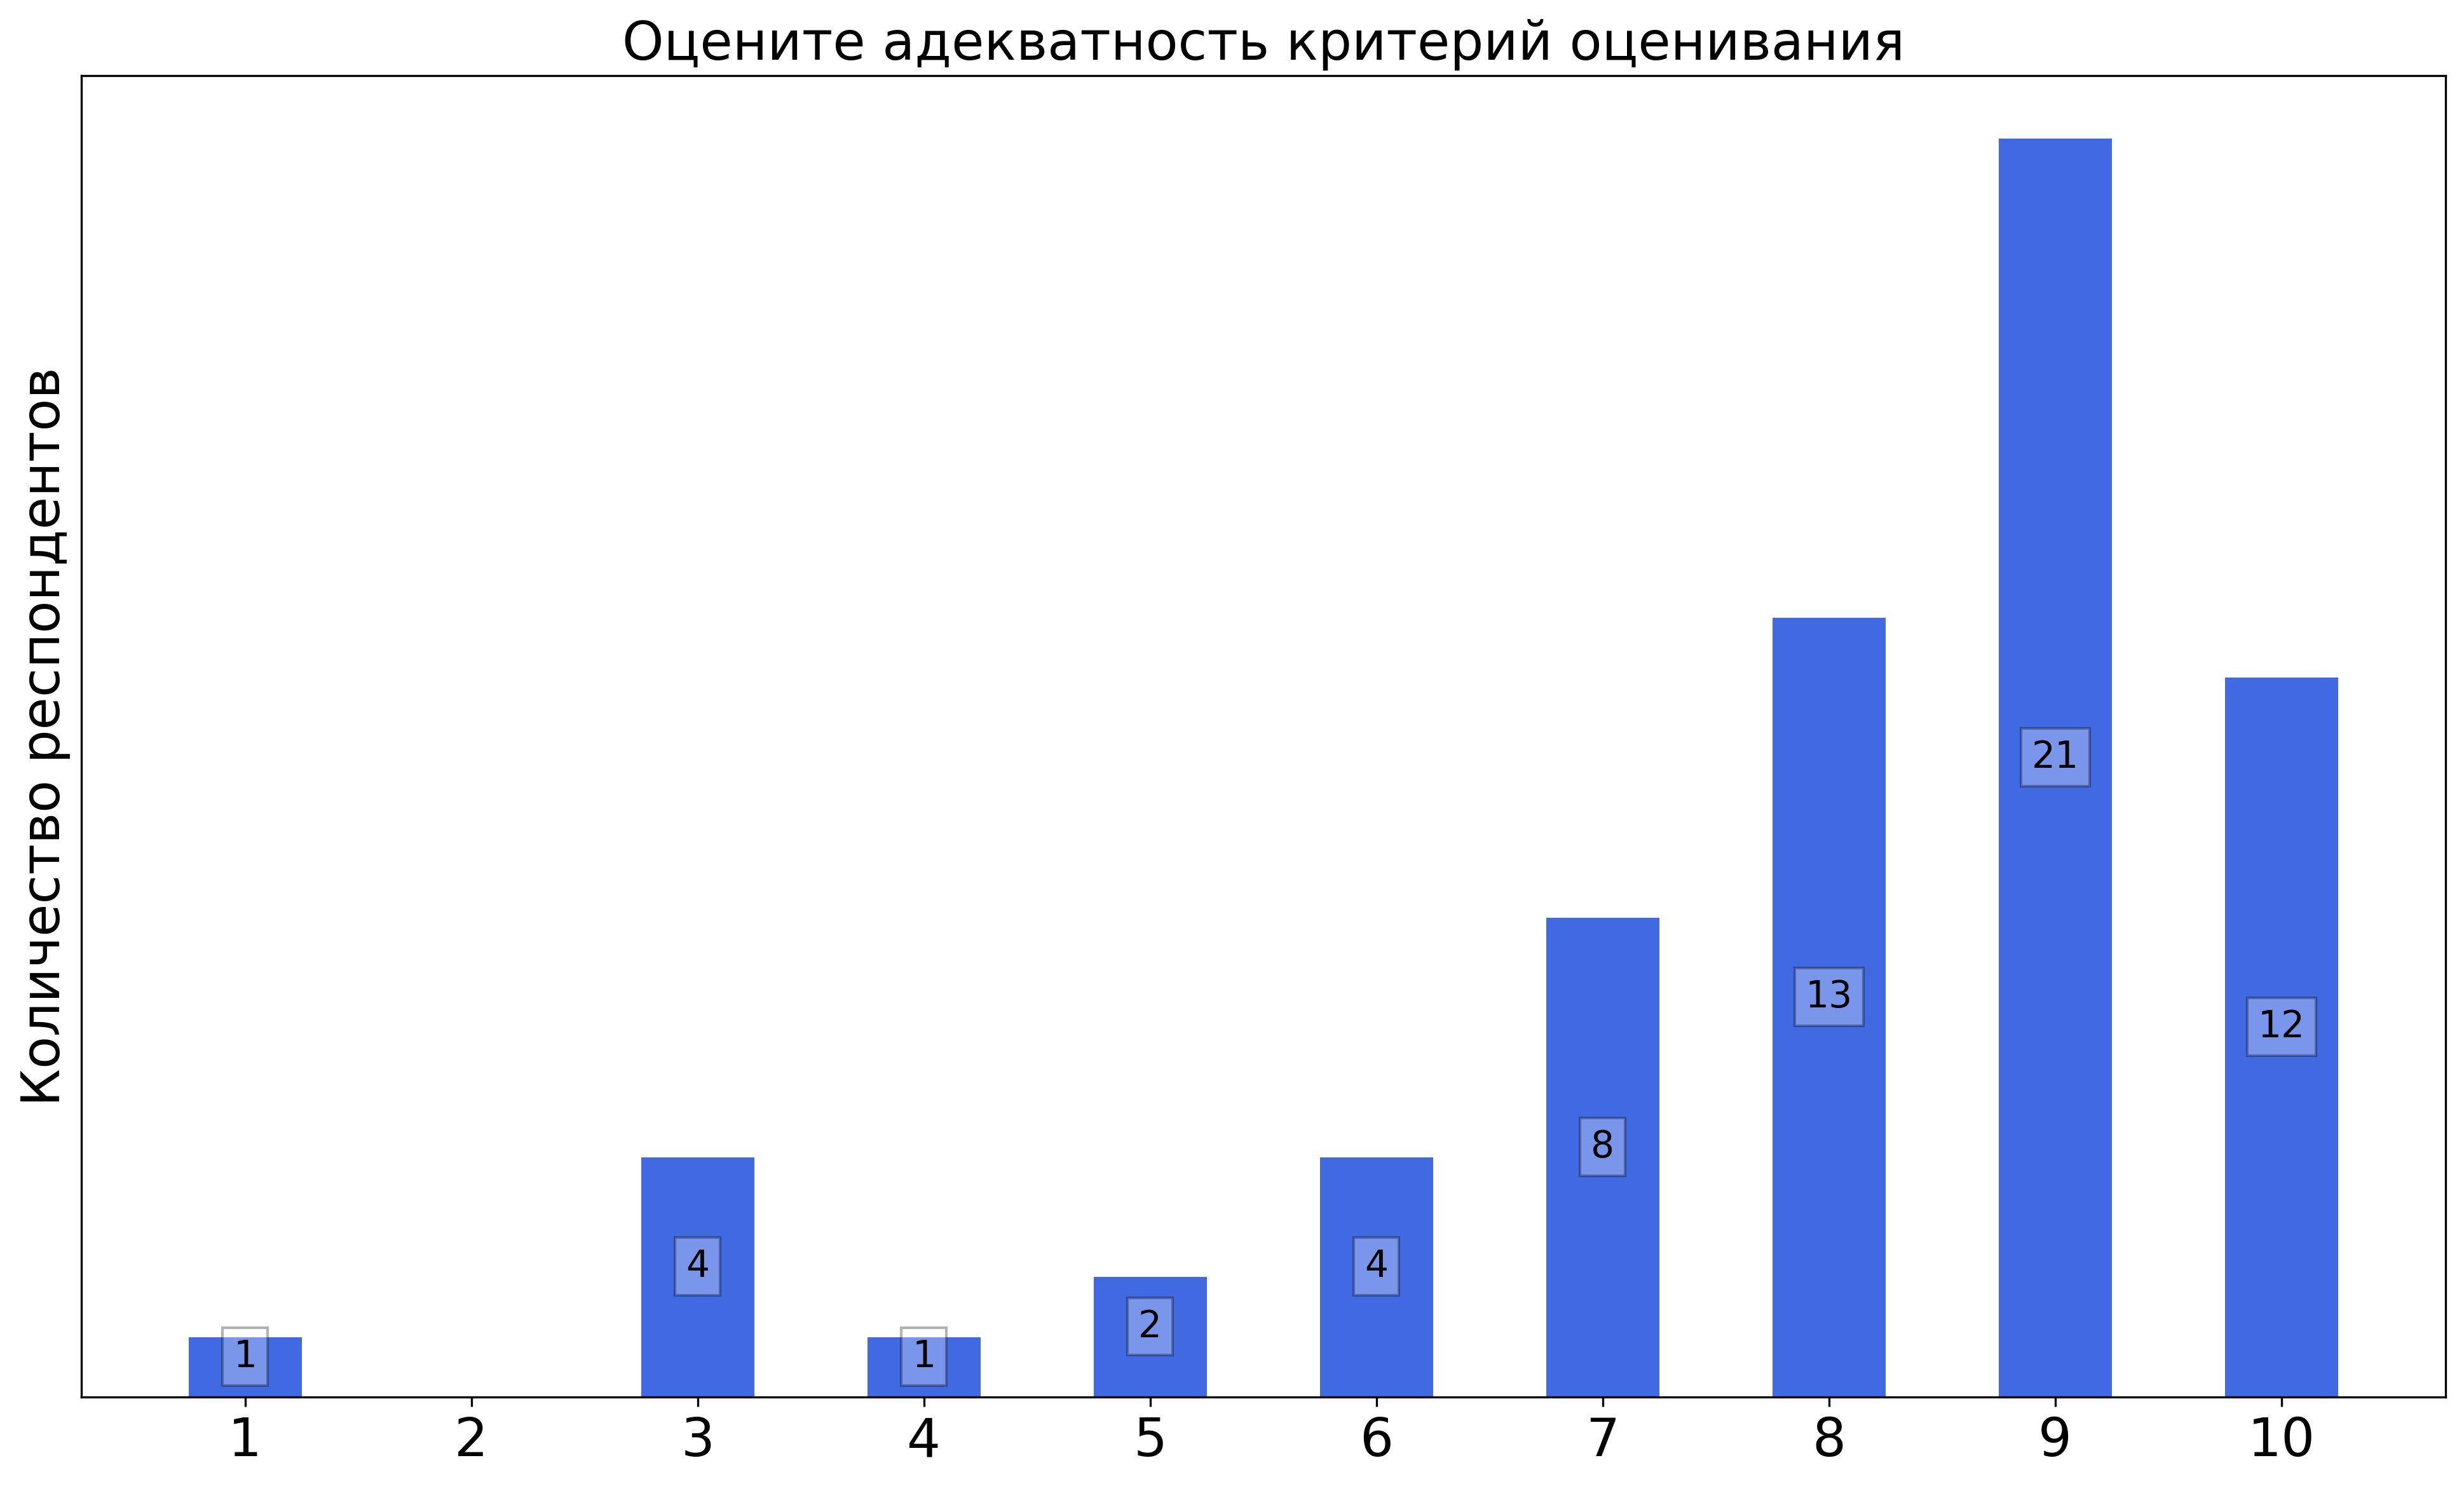
\includegraphics[width=\textwidth]{images/1 course/Аналитическая геометрия/general-1.png}
			\end{subfigure}	
		\end{figure}

	\subsubsection{Материалы, использумые респондентами при изучении курса}

		\begin{figure}[H]
			\centering
			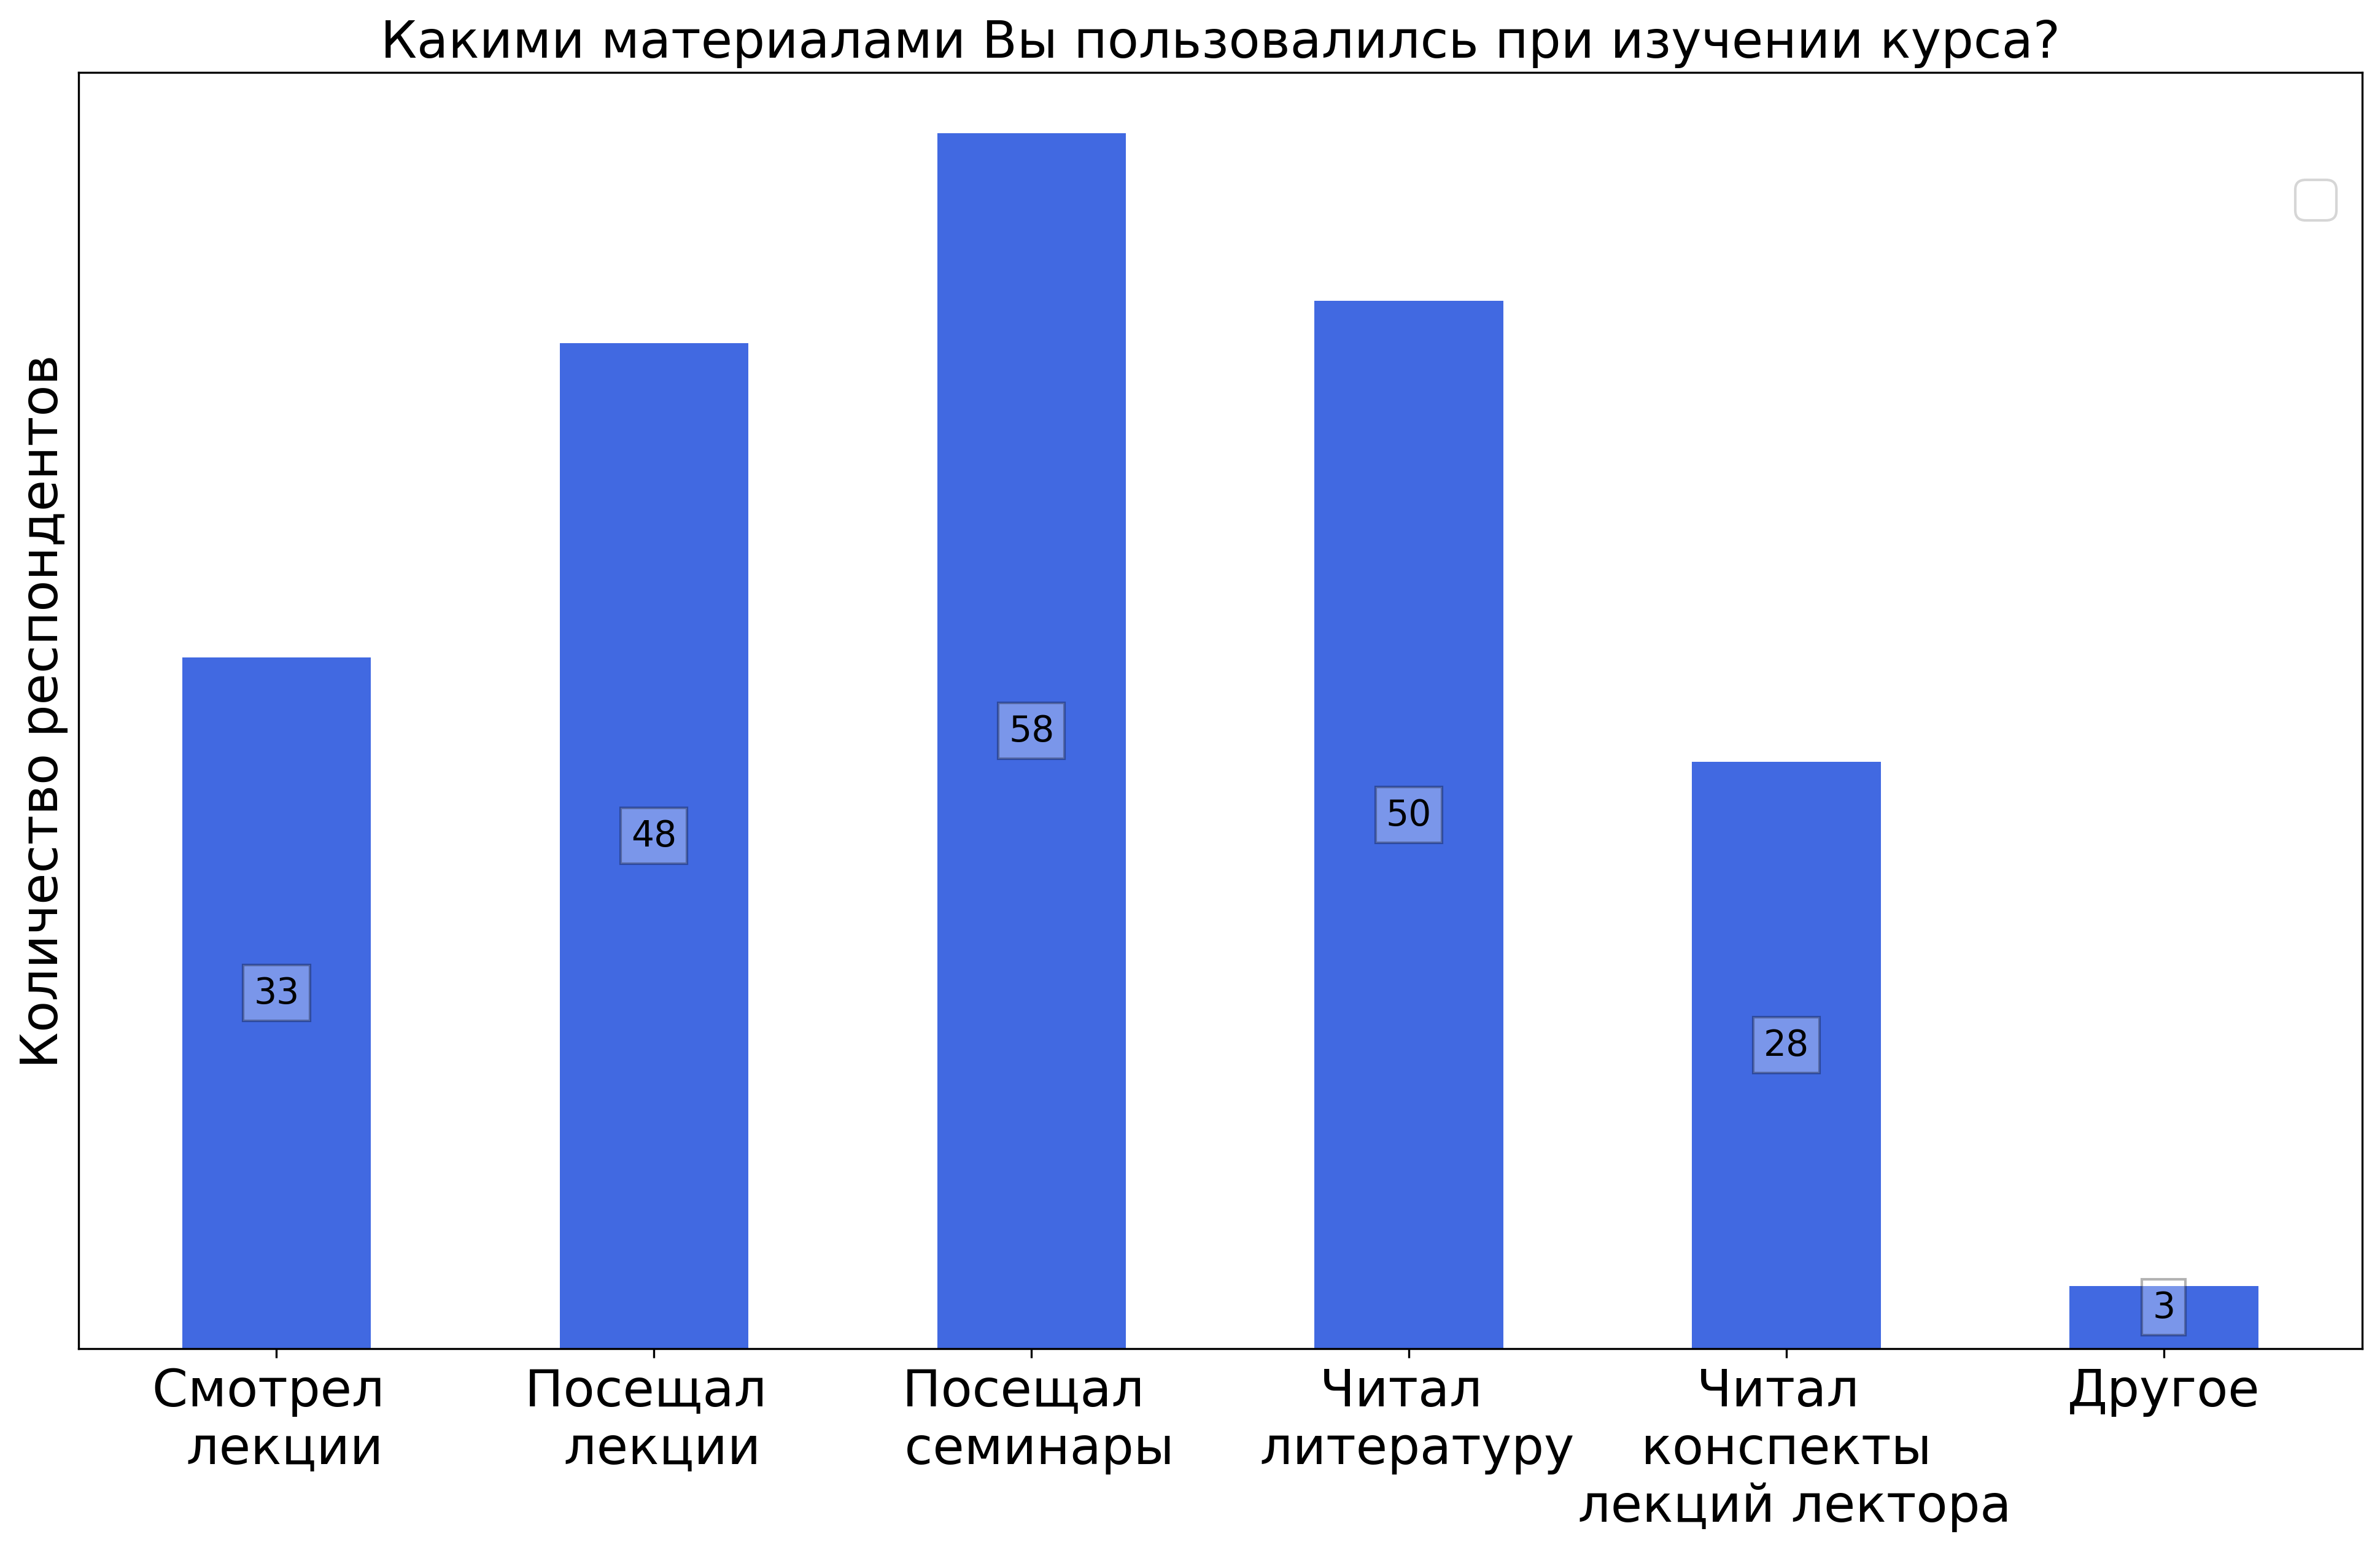
\includegraphics[width = 0.45\textwidth]{images/1 course/Аналитическая геометрия/materials.png}
		\end{figure}

		\textit{В качестве других источников информации студенты указали:} 
		\begin{itemize}
			\item материалы из интернета;
			\item лекции Сергея Жесткова.
		\end{itemize}

	\subsubsection{Отзыв студентов о лекциях. Лектор: Чубаров И.А.}

		\begin{figure}[H]
			\centering
            \begin{subfigure}[b]{0.45\textwidth}
				\centering
				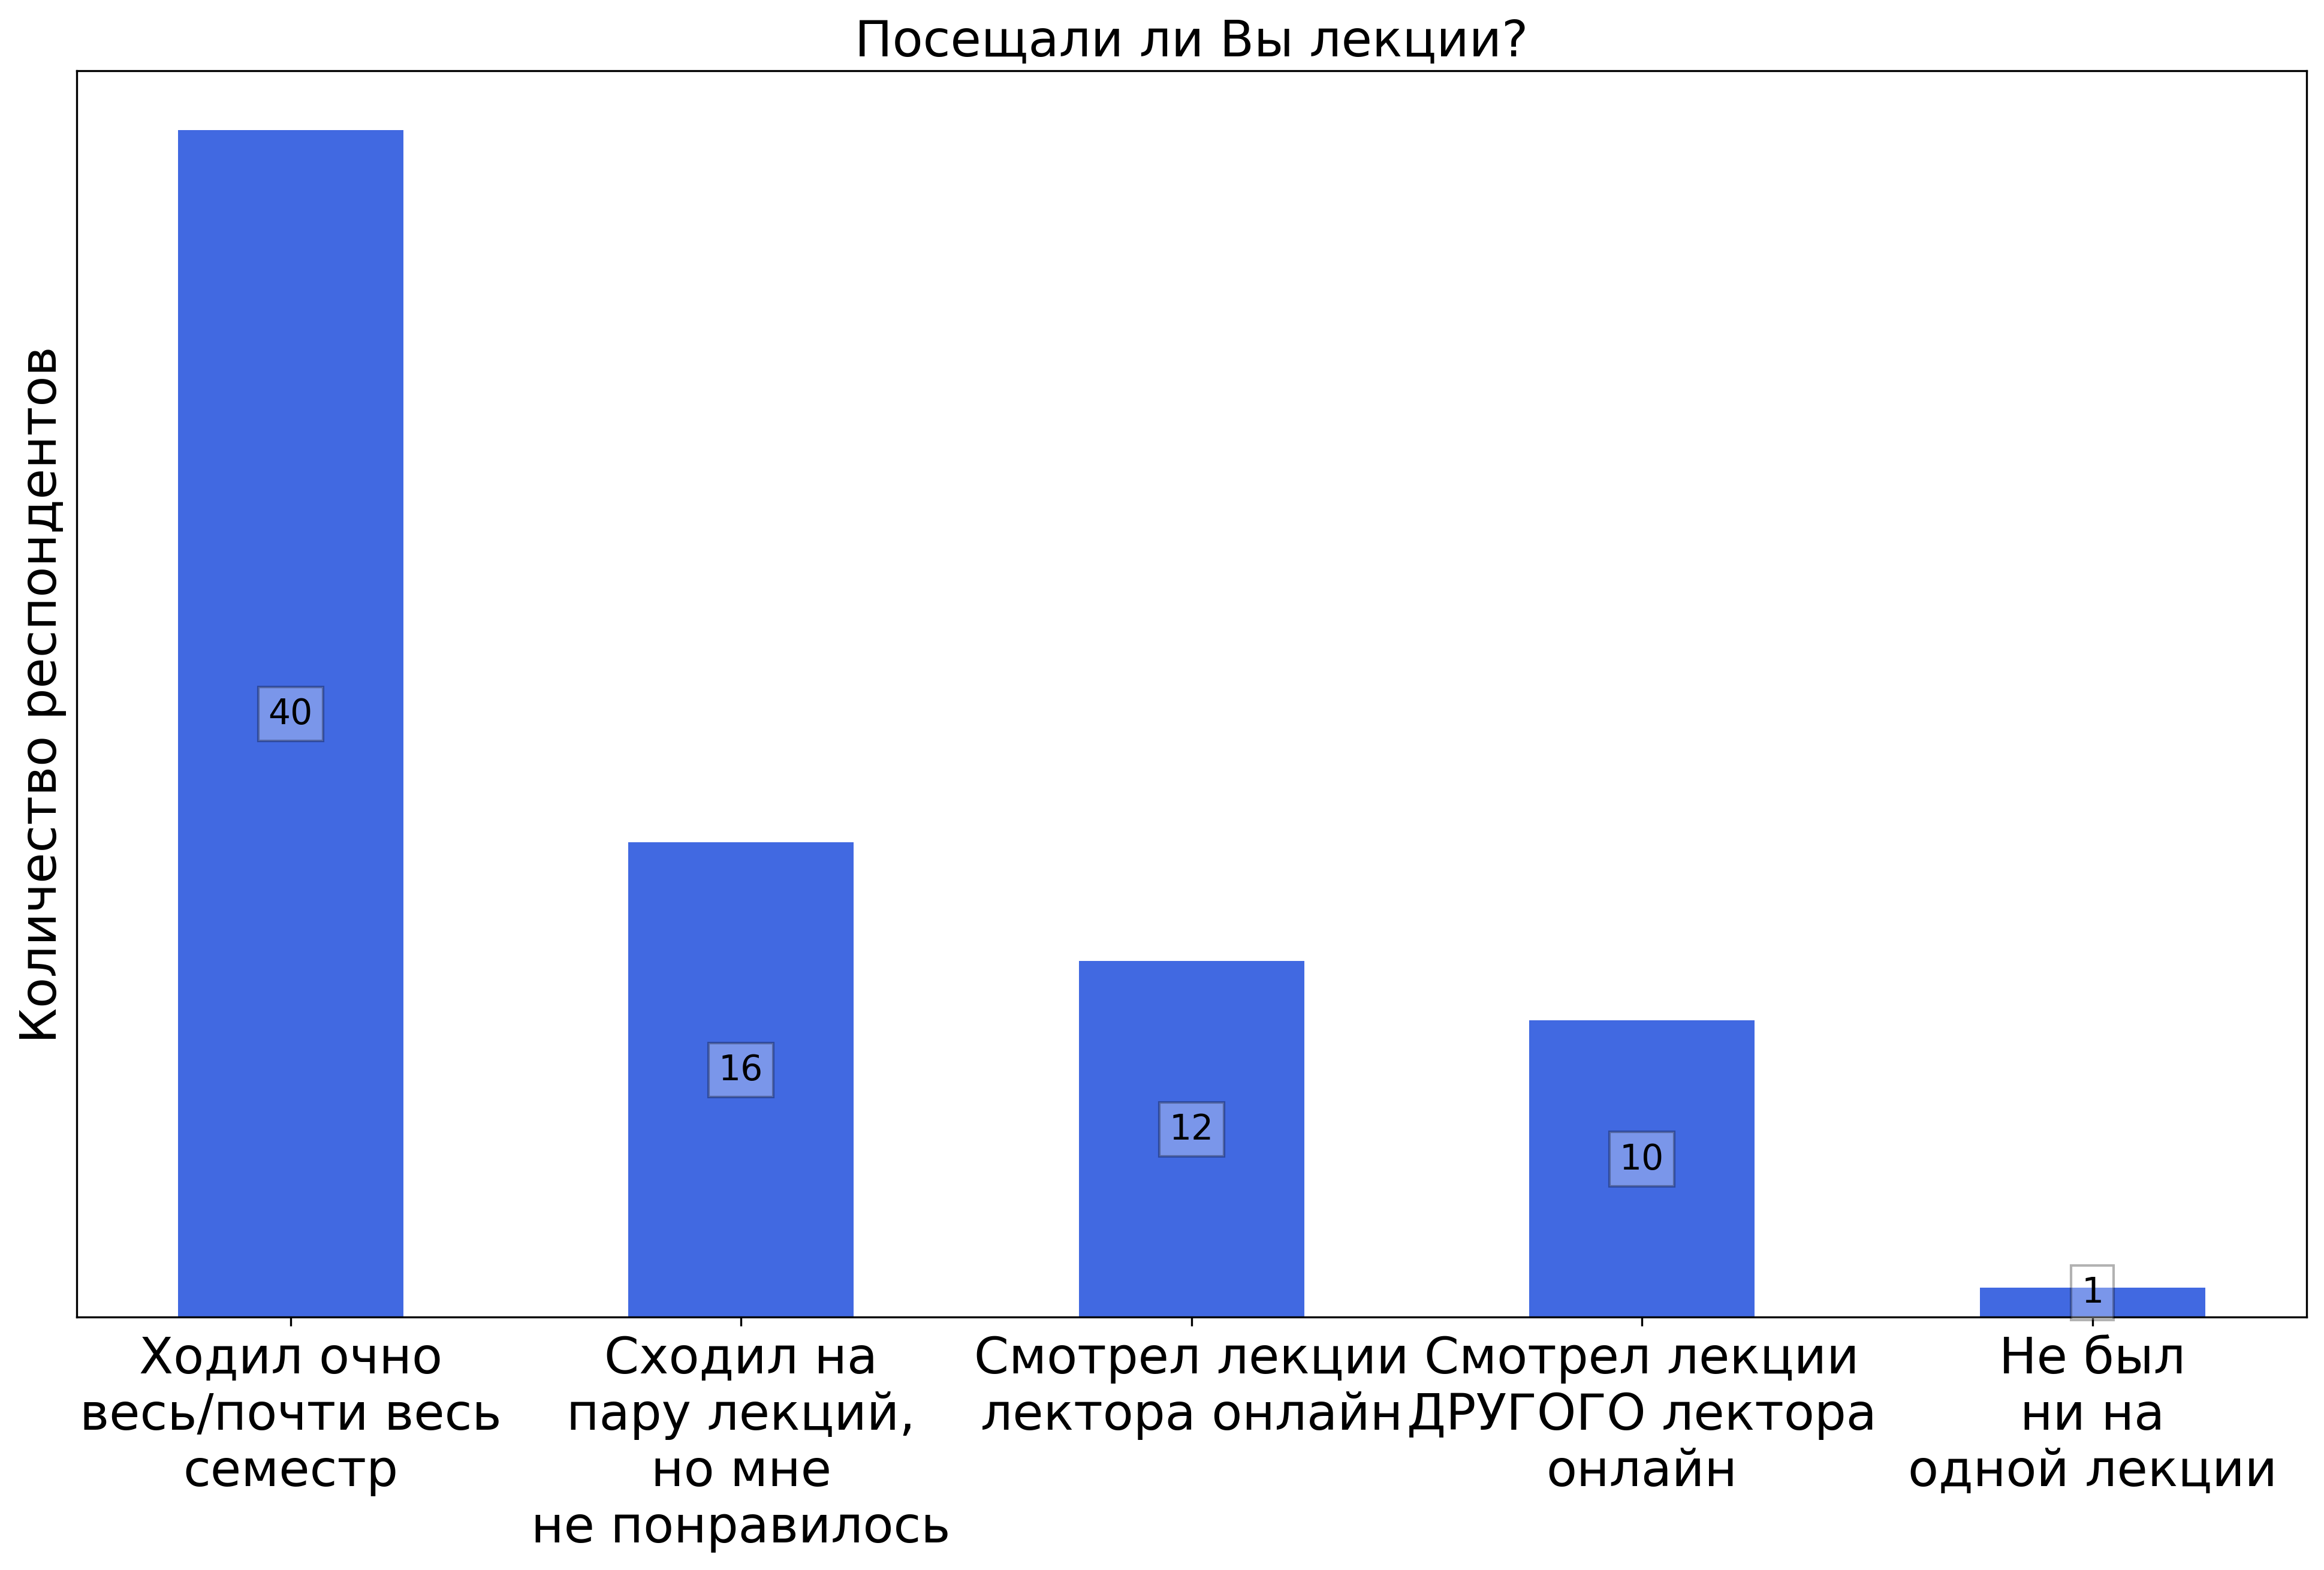
\includegraphics[width=\textwidth]{images/1 course/Аналитическая геометрия/lecturer-questions-Чубаров И.А.-0.png}
			\end{subfigure}
			\begin{subfigure}[b]{0.45\textwidth}
				\centering
				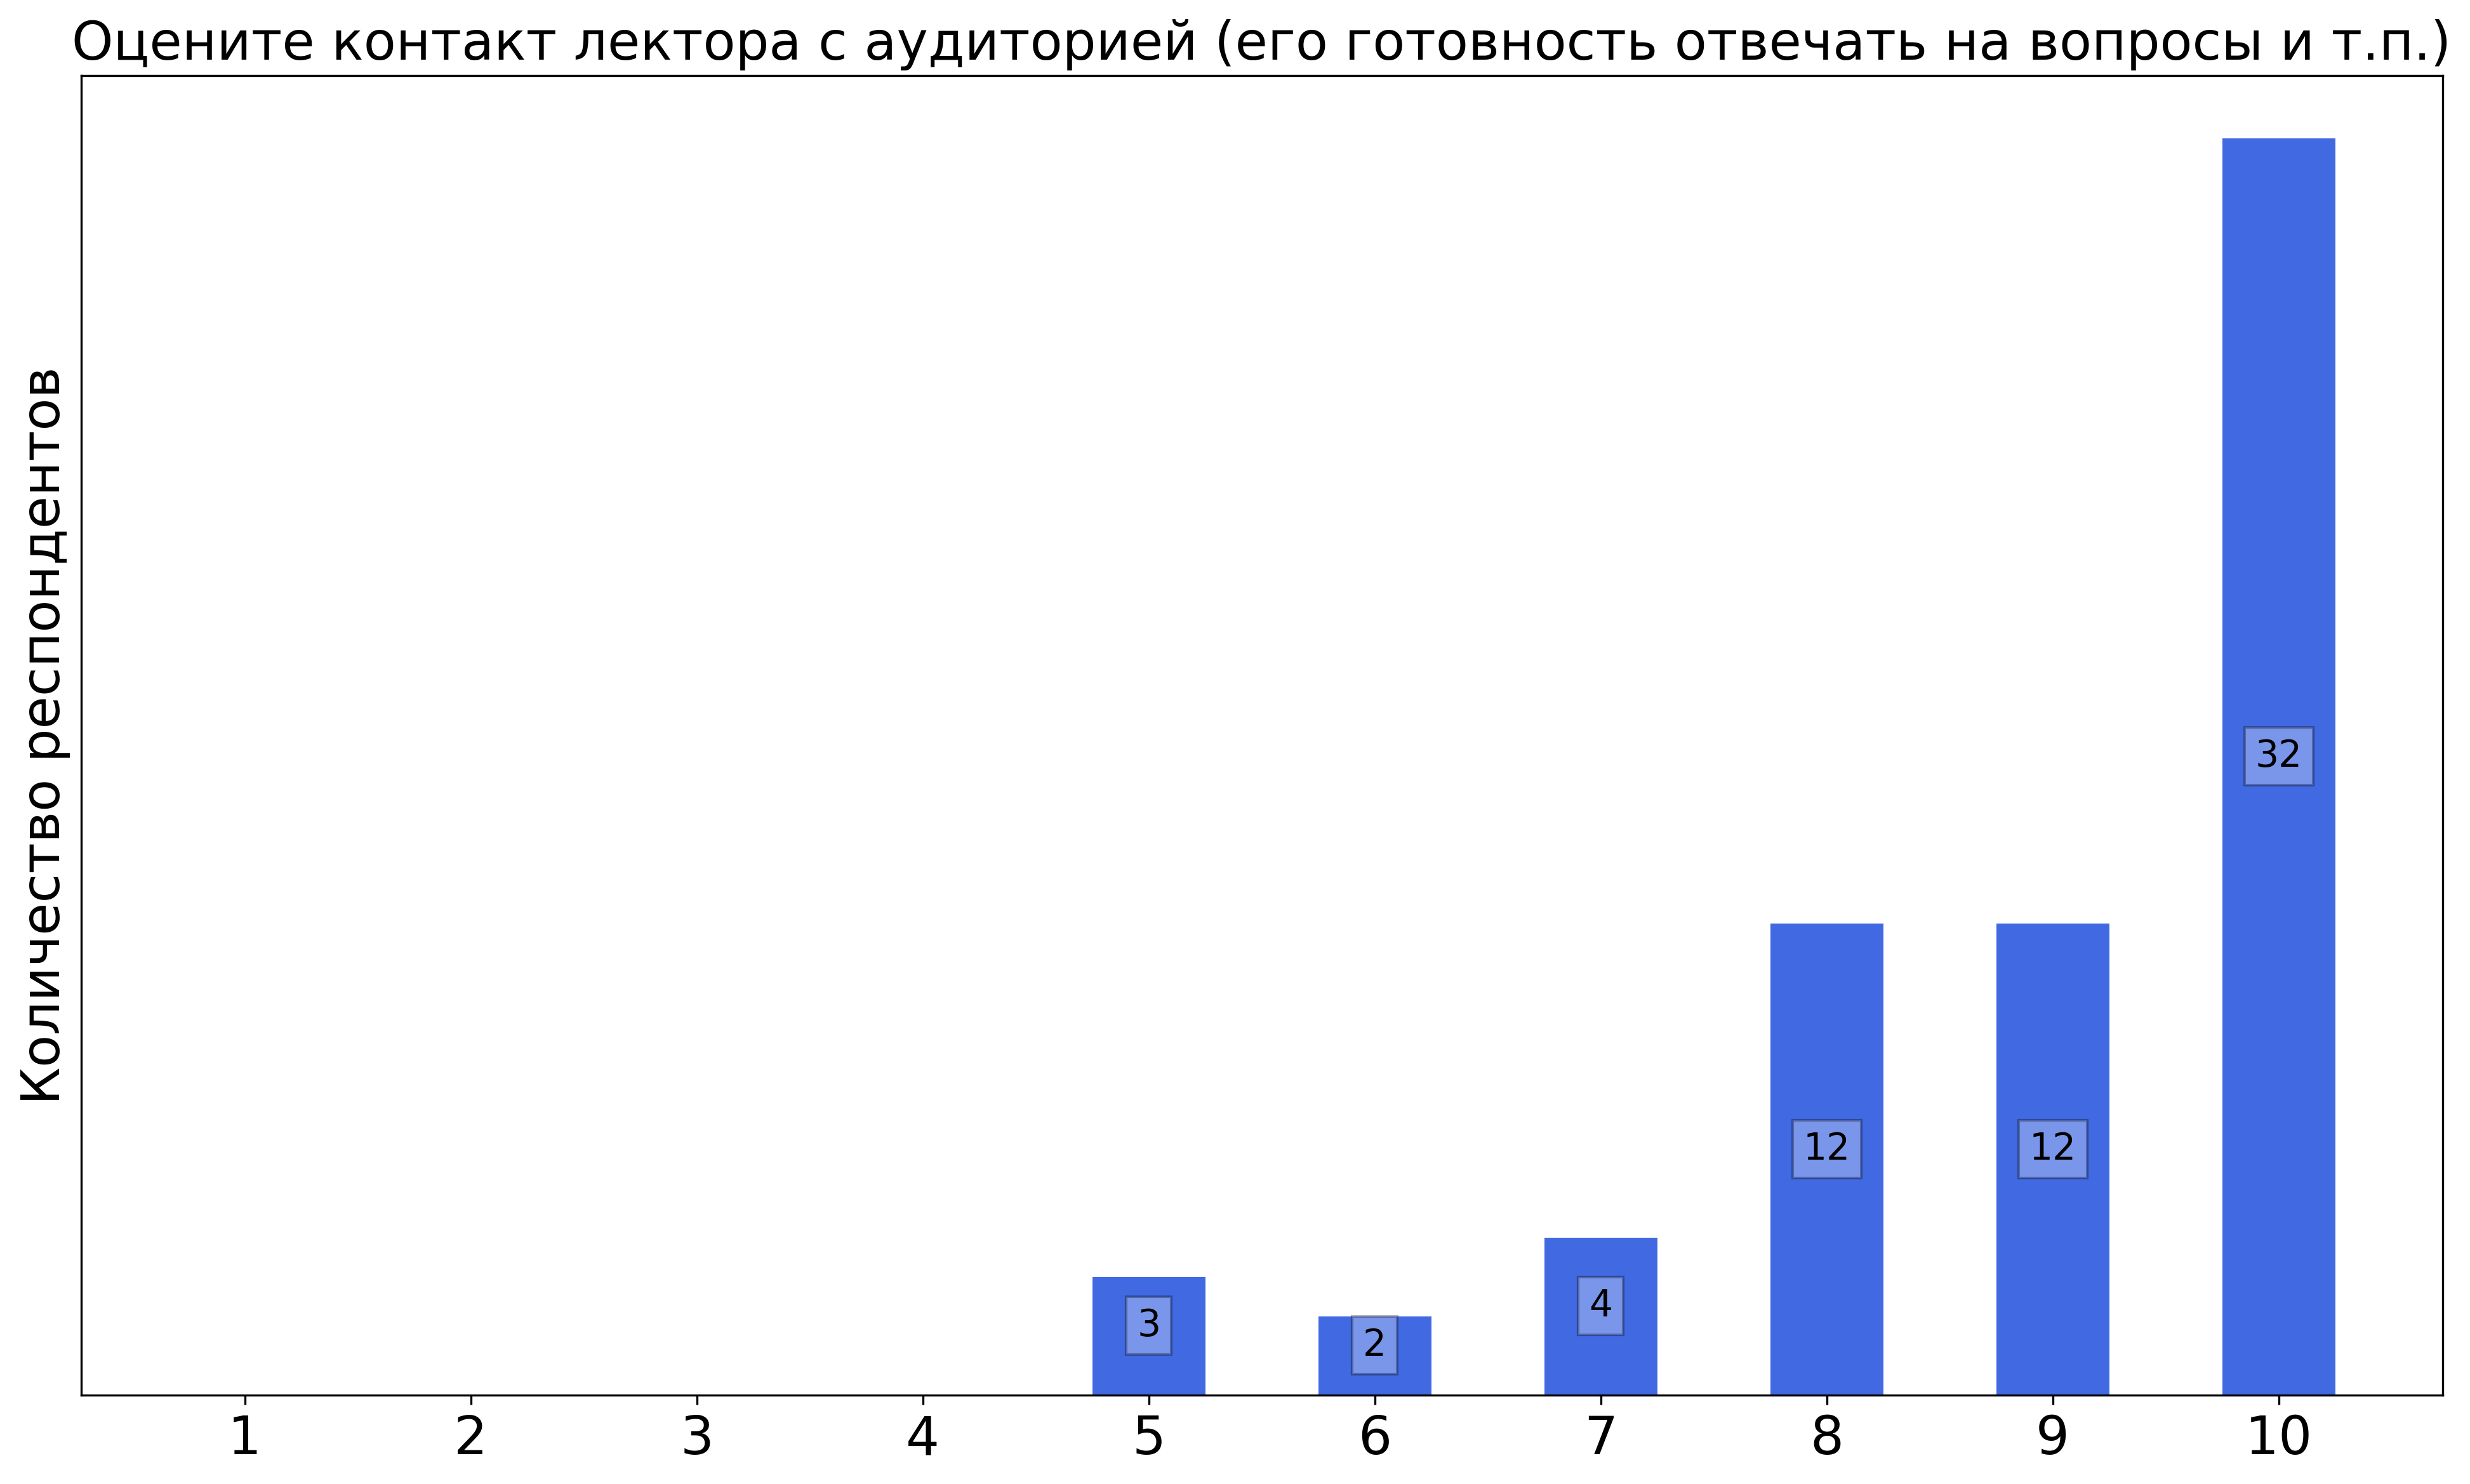
\includegraphics[width=\textwidth]{images/1 course/Аналитическая геометрия/lecturer-marks-Чубаров И.А.-0.png}
			\end{subfigure}
			\begin{subfigure}[b]{0.45\textwidth}
				\centering
				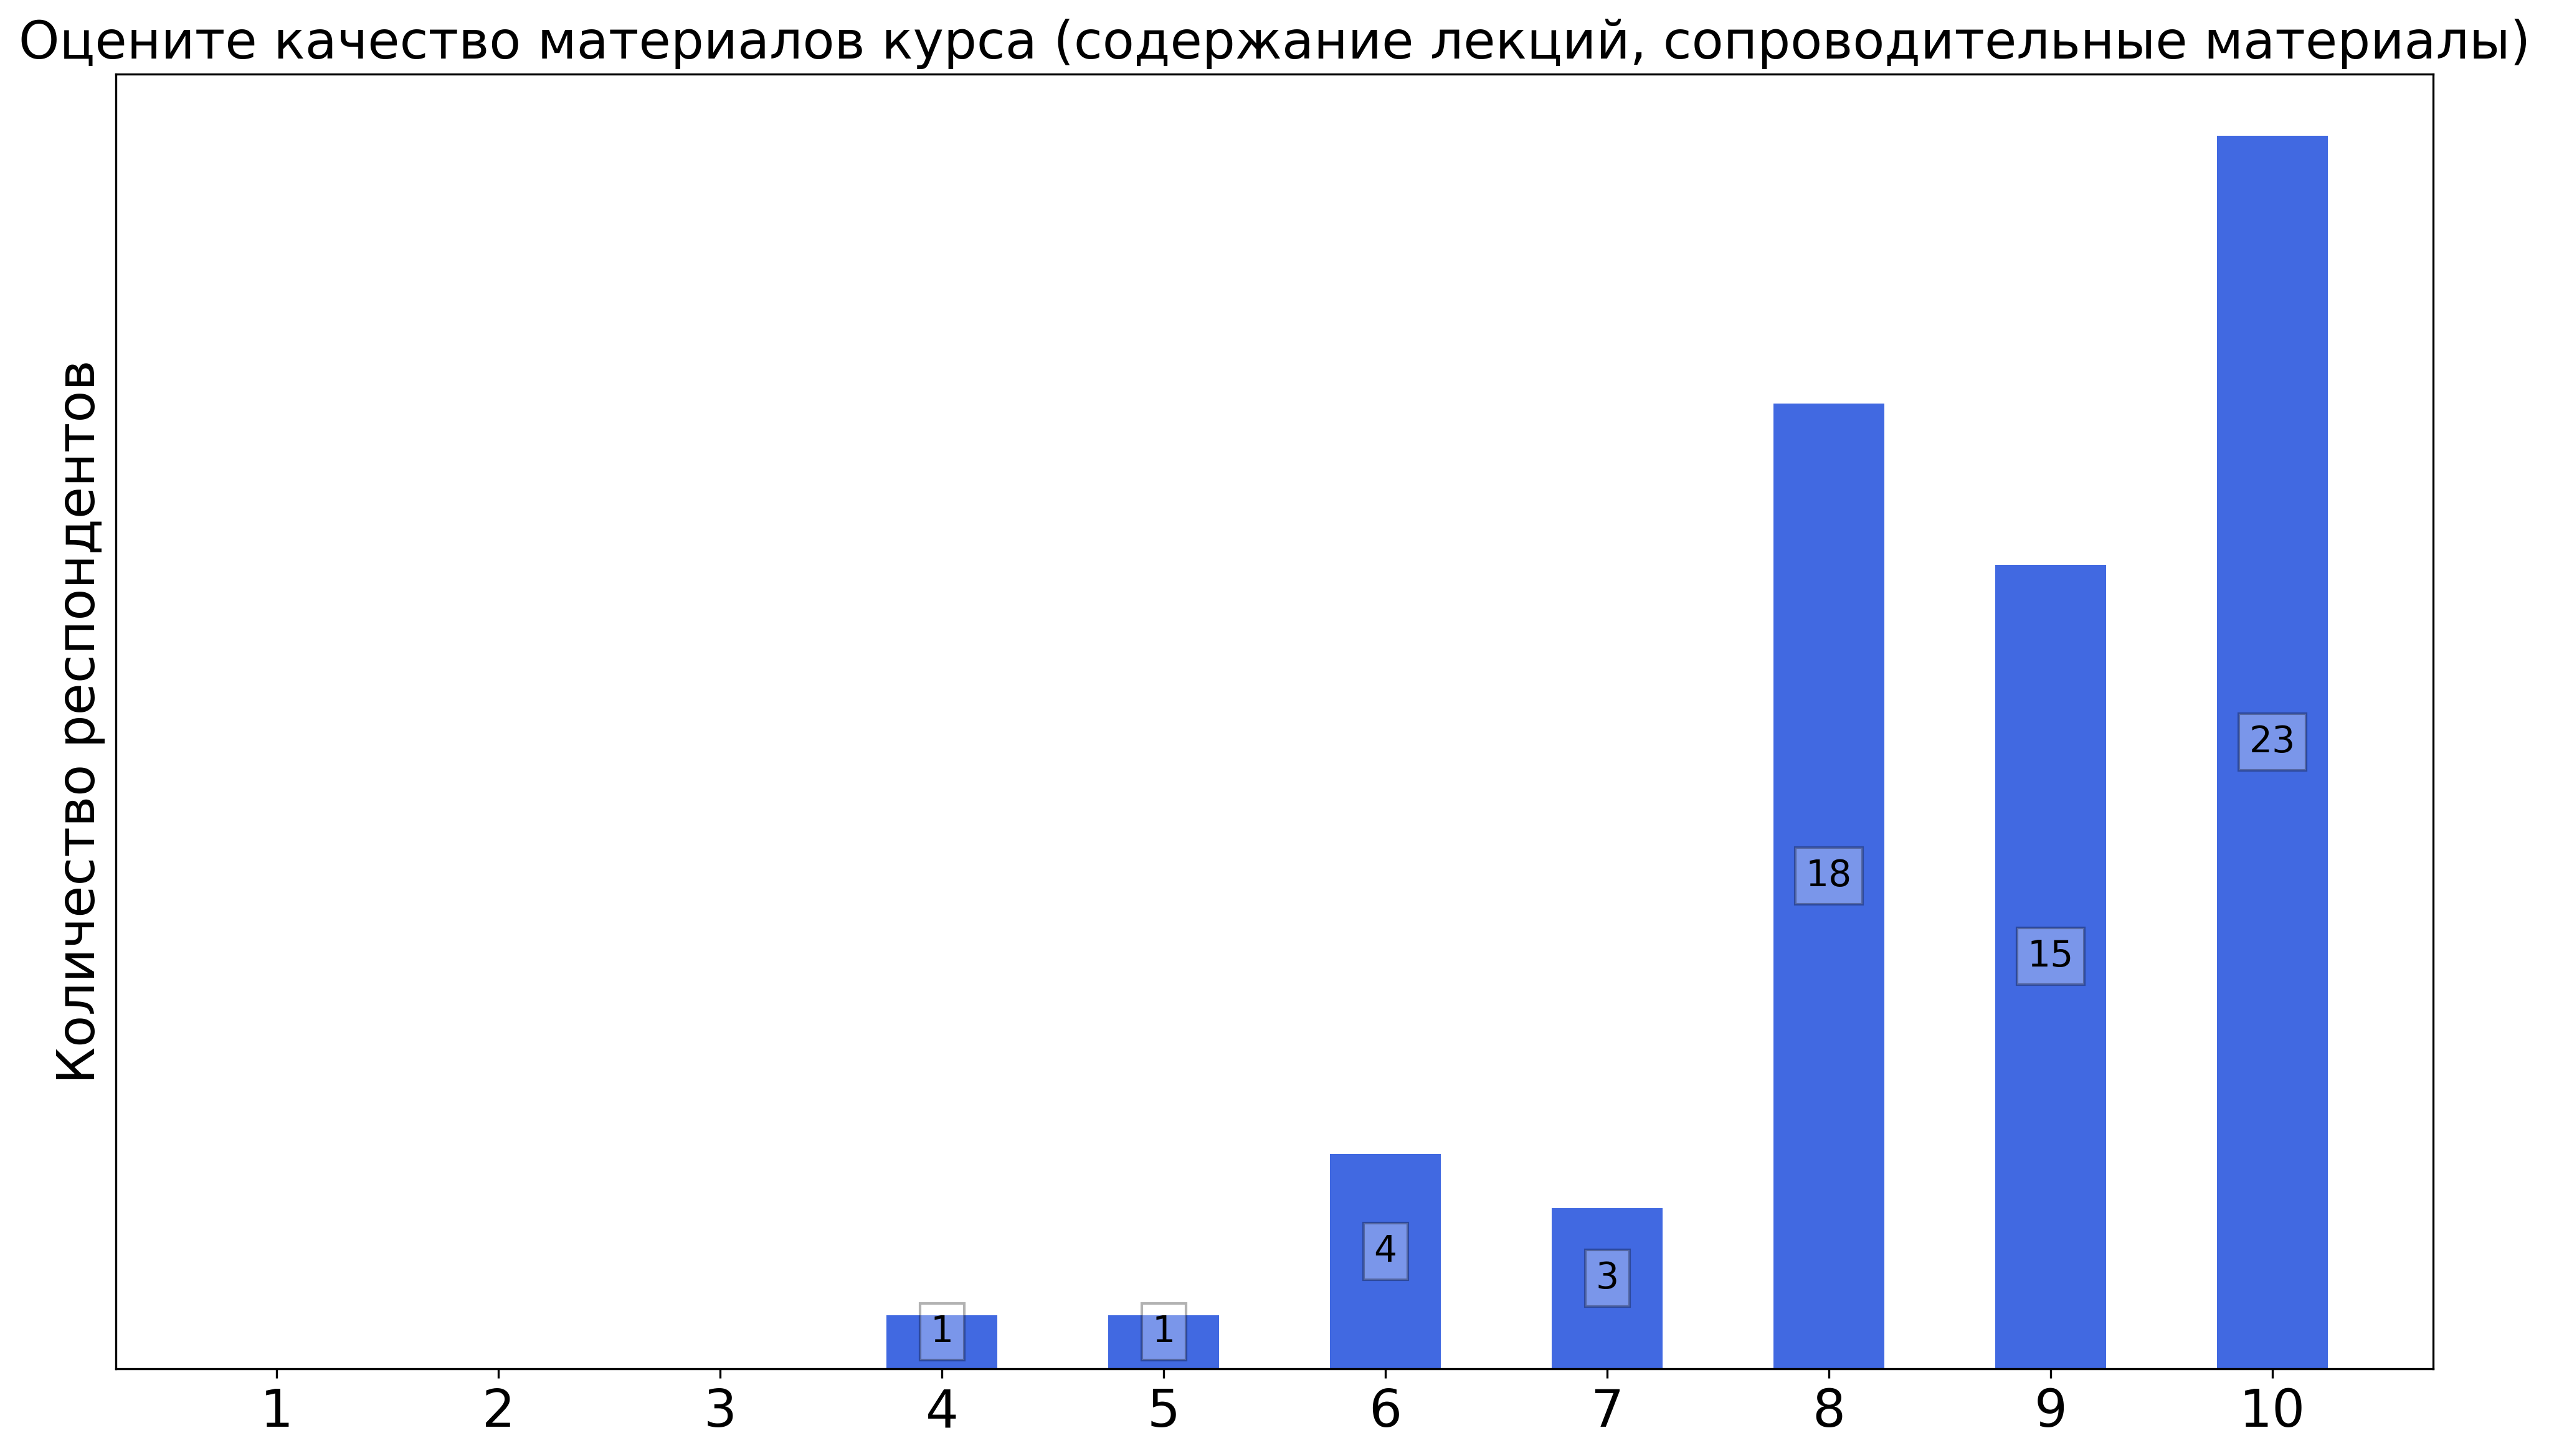
\includegraphics[width=\textwidth]{images/1 course/Аналитическая геометрия/lecturer-marks-Чубаров И.А.-1.png}
			\end{subfigure}
			\begin{subfigure}[b]{0.45\textwidth}
				\centering
				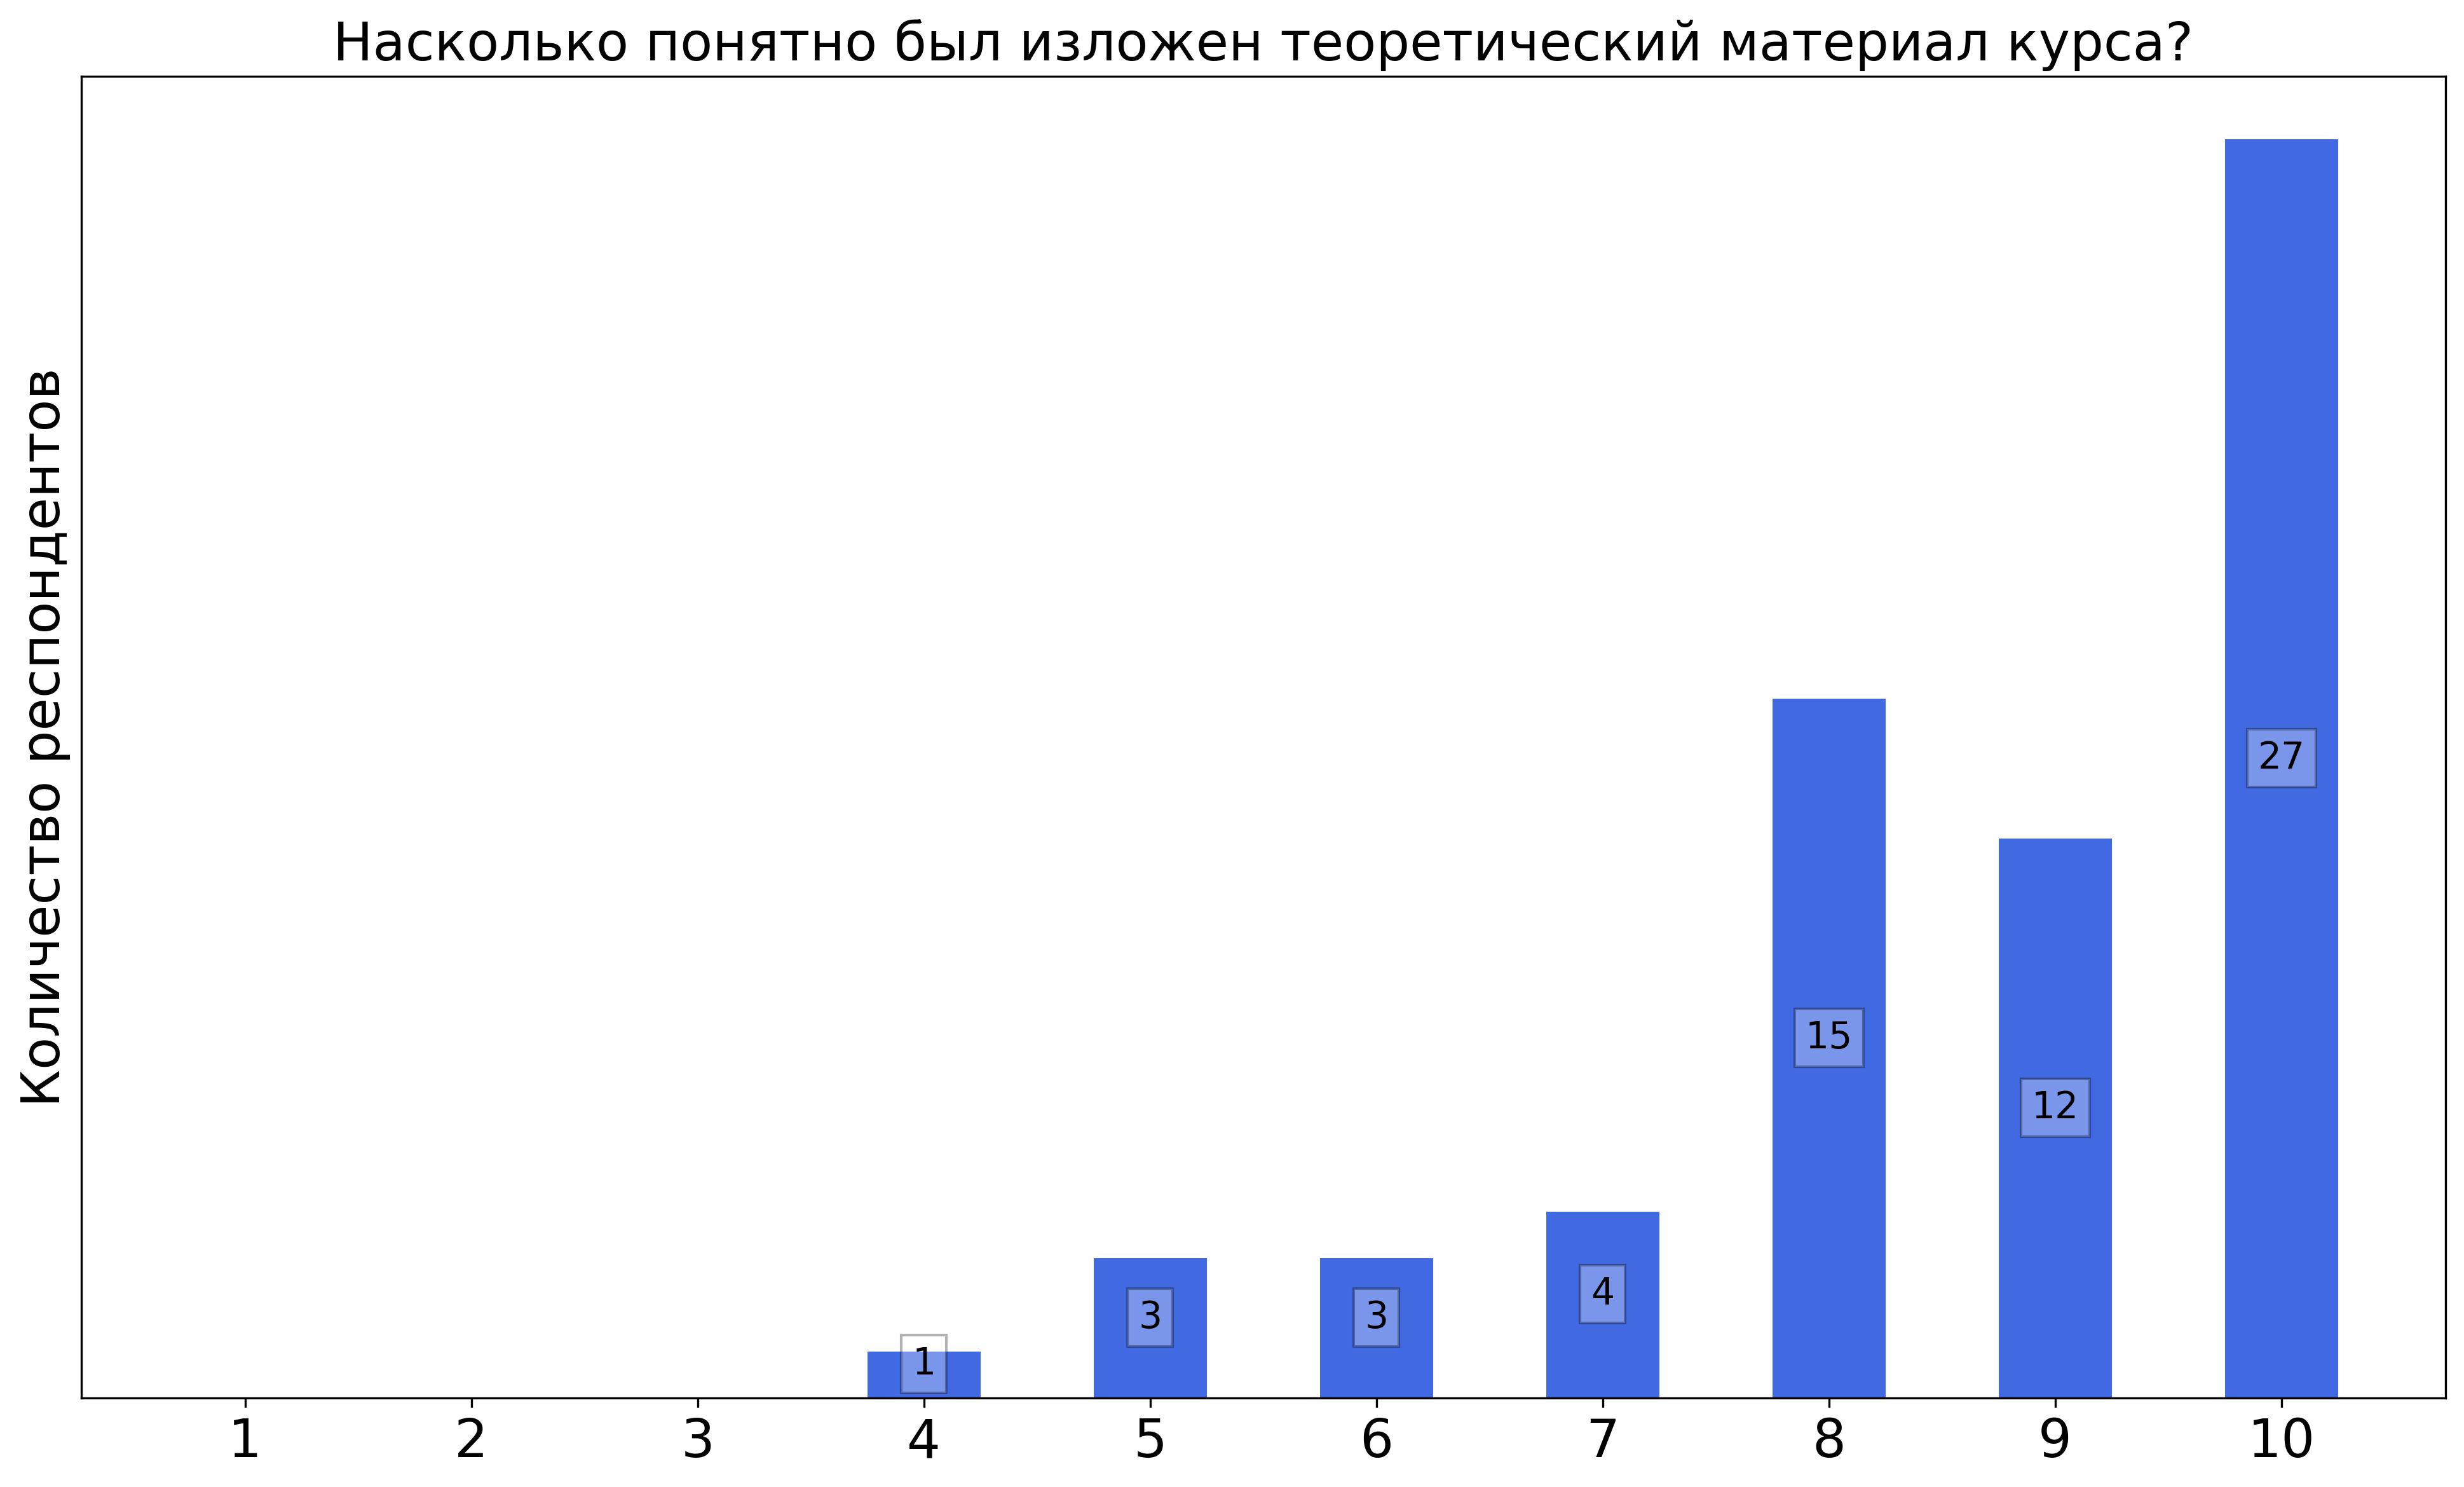
\includegraphics[width=\textwidth]{images/1 course/Аналитическая геометрия/lecturer-marks-Чубаров И.А.-2.png}
			\end{subfigure}
			\begin{subfigure}[b]{0.45\textwidth}
				\centering
				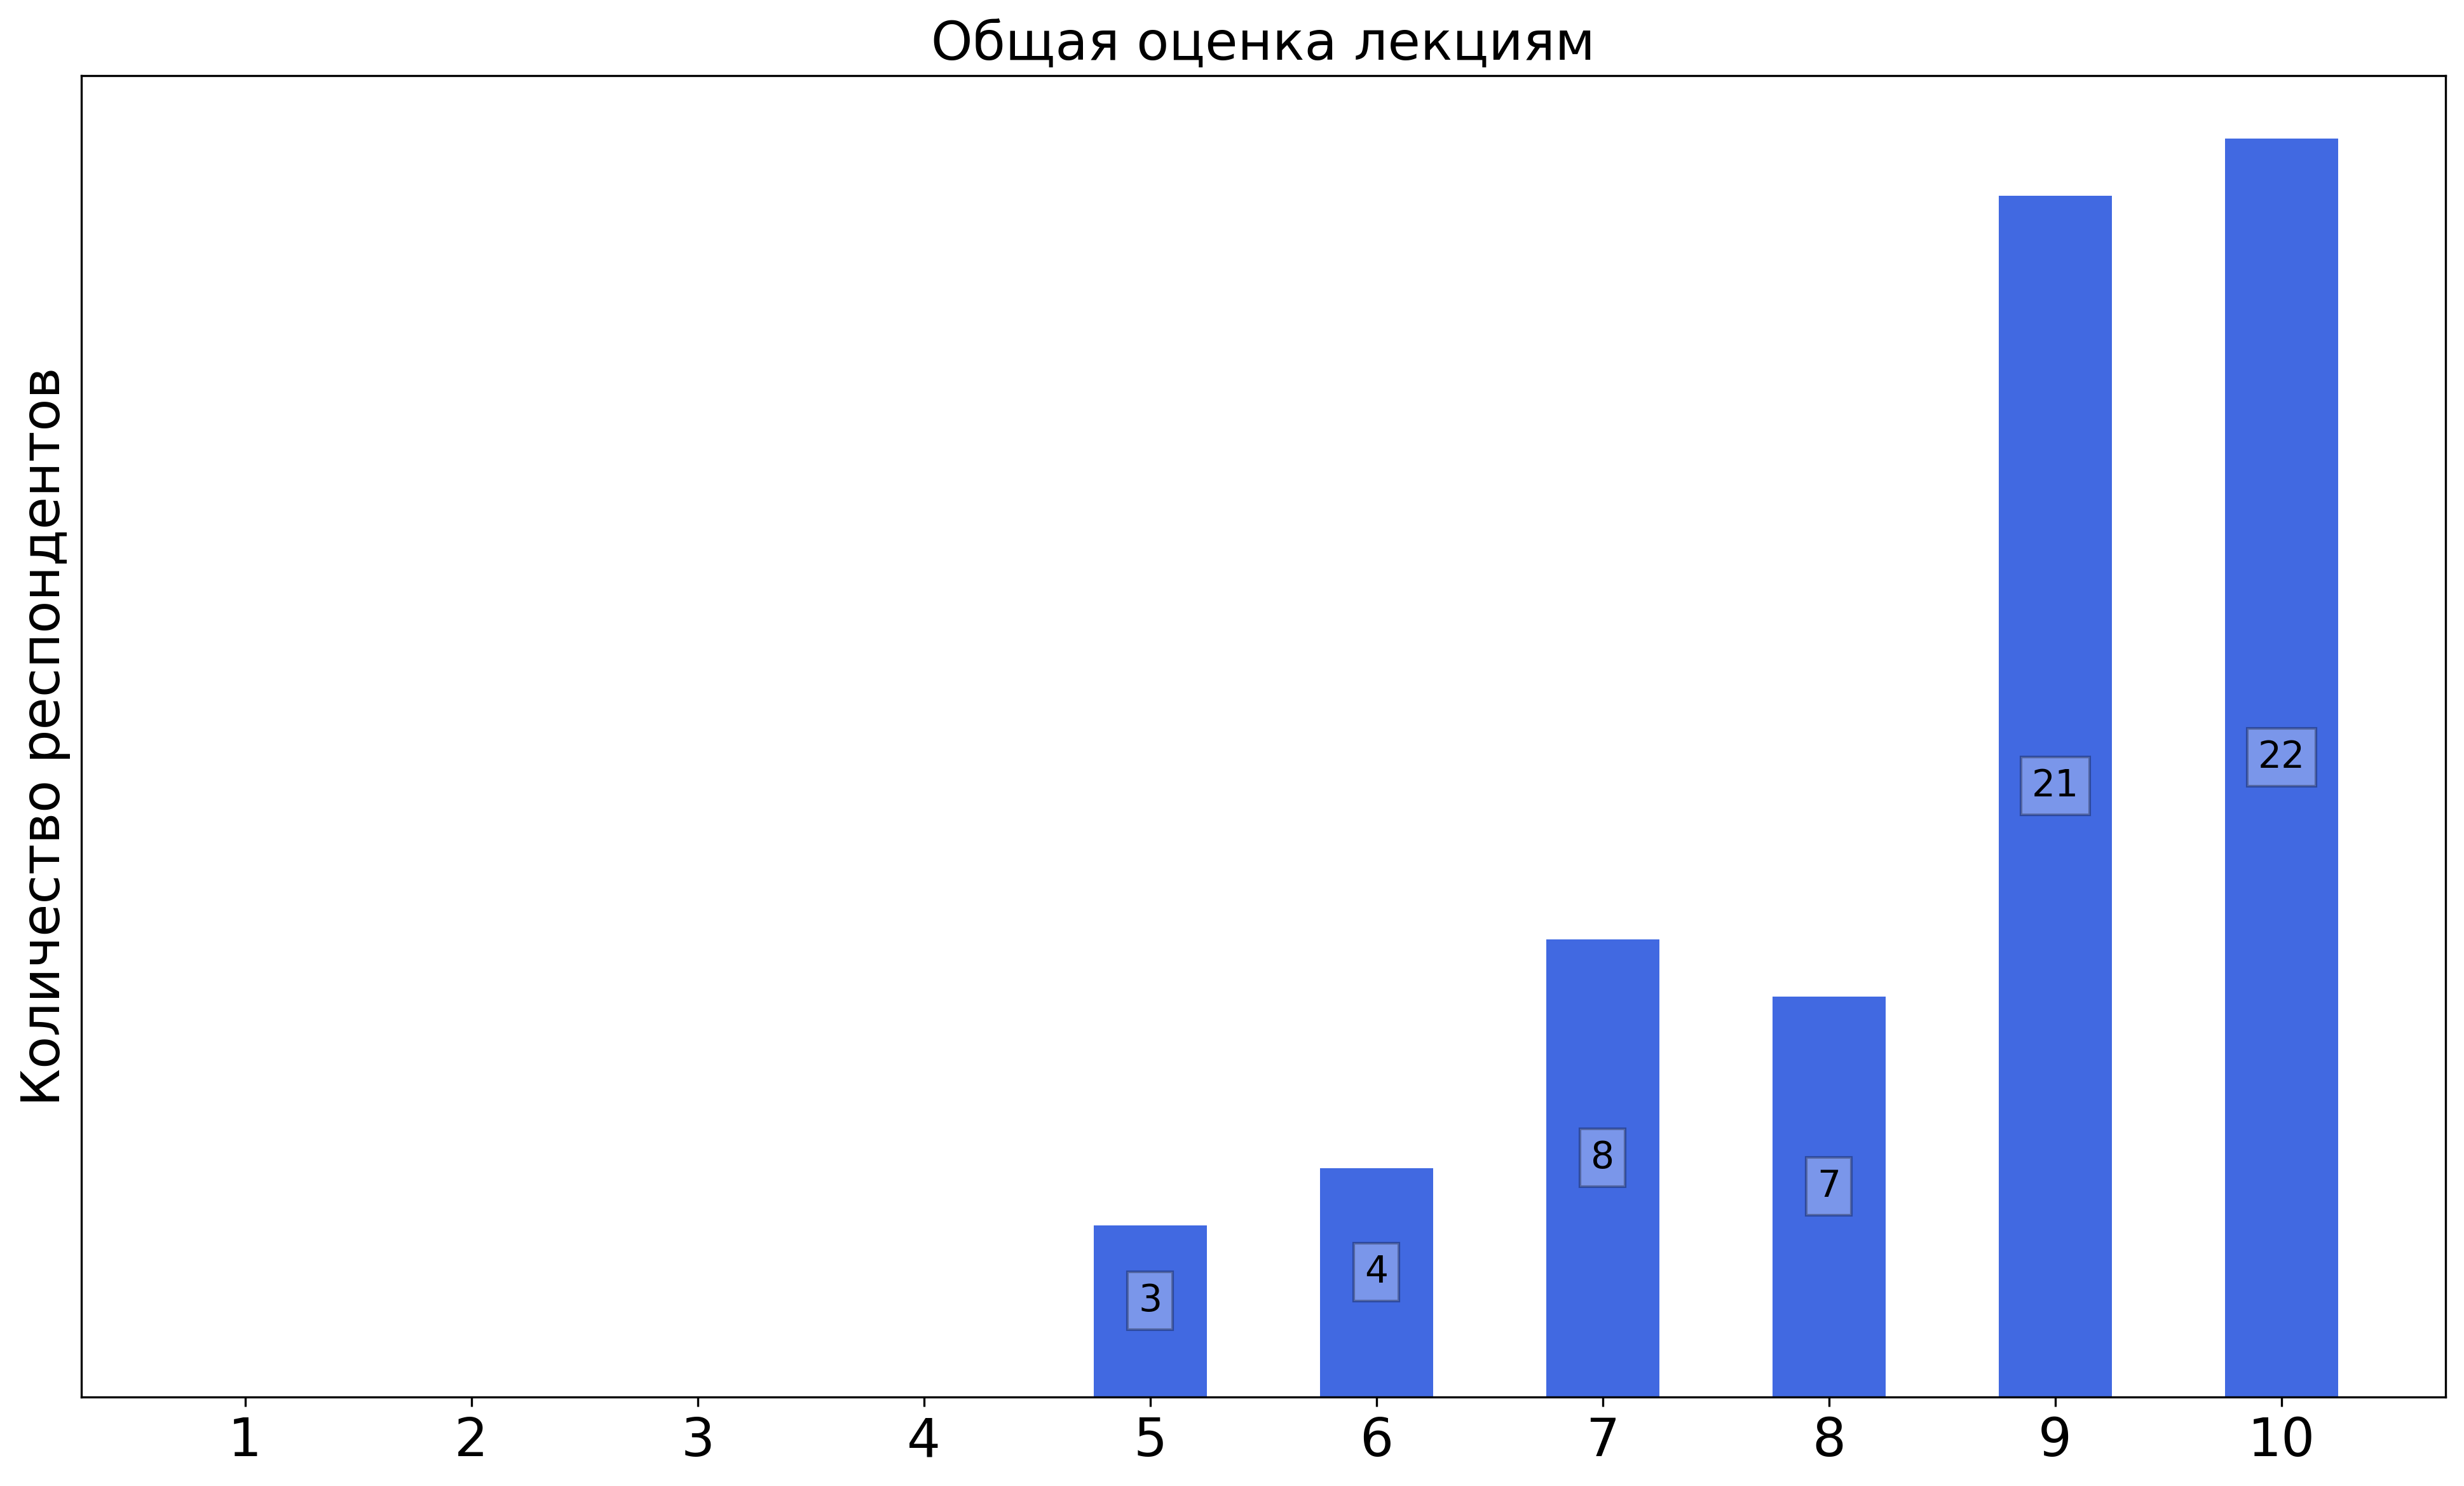
\includegraphics[width=\textwidth]{images/1 course/Аналитическая геометрия/lecturer-marks-Чубаров И.А.-3.png}
			\end{subfigure}
			\caption{Оценки респондентов о качестве преподавания лекций по курсу <<Аналитическая геометрия>>}
		\end{figure}

		\textbf{Комментарии студентов о лекциях\protect\footnote{сохранены оригинальные орфография и пунктуация}}    
            \begin{commentbox} 
                Замечательный лектор! Лучший из тех, которые у меня были за 1 семестр! Всегда готов ответить на вопросы, объясняет очень понятно и доступно. Очень добрый, отзывчивый и понимающий человек. На экзамене оценивает лояльно, сдавать одно удовольствие 
            \end{commentbox} 
        
            \begin{commentbox} 
                Говорит медленно и понятно. Всегда готов объяснить и ответить на вопросы. Отдельные моменты из программы объяснены не очень хорошо, но это неизбежно и не очень критично 
            \end{commentbox} 
        
            \begin{commentbox} 
                Говорит тихо, с микрофоном нормально  
            \end{commentbox} 
        
            \begin{commentbox} 
                Лектор супер. Да, может другие скажут, что темп медленный, но зато много доп инфы 
            \end{commentbox} 
        
            \begin{commentbox} 
                Отличный лектор. К сожалению, не успел изложить материал целиком. 
            \end{commentbox} 
        
            \begin{commentbox} 
                В общем, Игорь Андреевич - хороший лектор. Это я раздолбай. 
            \end{commentbox} 
        
            \begin{commentbox} 
                один из лучших лекторов первого семестра 
            \end{commentbox} 
        
            \begin{commentbox} 
                Не все рассказывается, что нужно на экзамене  
            \end{commentbox}  
        
            \begin{commentbox} 
                После впечатления от матана очень неструктурированно, слишком разбросан материал, часто рассказывается неструктурированно, большой минус, когда сложно понимать материал в принципе. 
            \end{commentbox} 
        
            \begin{commentbox} 
                Отличный лектор. Есть только один недостаток: не получается записать лекцию и понять её до конца одновременно, так как сначала пытаешься разобрать, что написано (из-за специфики терминов в большинстве случаев), потом пытаешься осознать материал и только после переписываешь. Но благодаря ответам на вопросы становиться ГОРАЗДО лучше. Полное понимание приходит после семинаров или после повторного просмотра лекций 
            \end{commentbox} 
        
            \begin{commentbox} 
                Чувствуется опыт работы лектора. Материал преподносится уверенно и доступно. По материалам этих лекций можно спокойно готовиться к сдаче экзамена. Единственный минус - отставание от программы (из-за чего часть материала была рассказана уже на дополнительных лекциях) 
            \end{commentbox} 
        
            \begin{commentbox} 
                Очень тихо говорит, в аудитории практически ничего не было слышно 
            \end{commentbox} 
        
            \begin{commentbox} 
                Игорь Андреевич читает довольно понятно, отпускает бородатые анекдоты, но не успевает за программой, кроме того оставляет половину доказательств на потом (которого никогда не будет), причём это обычно самые сложные теоремы.   
            \end{commentbox} 
        
            \begin{commentbox} 
                самые интересные лекции первого семестра 
            \end{commentbox} 
        
            \begin{commentbox} 
                Лекции Чубарова И.А. - синтетический курс ангема из самых разных источников (какой-то фрагмент лекции взят у Беклемишева Д.В., какой-то - у Умнова А.Е., какой-то - у Кострикина). Также, много дополнительных материалов, которые, с одной стороны, могут уже опытному в теме помочь разобраться в некоторых нюансах, а с другой, могут запутать ещё не опытного. Но в целом, выше написанное касается больше всего подготовки к экзаменам - приходится так же "синтезировать" 
            \end{commentbox}


    \subsubsection{Отзыв студентов о семинарах. Семинарист: Агаханова Я.С.}
        \begin{figure}[H]
            \centering
            \begin{subfigure}[b]{0.45\textwidth}
                \centering
                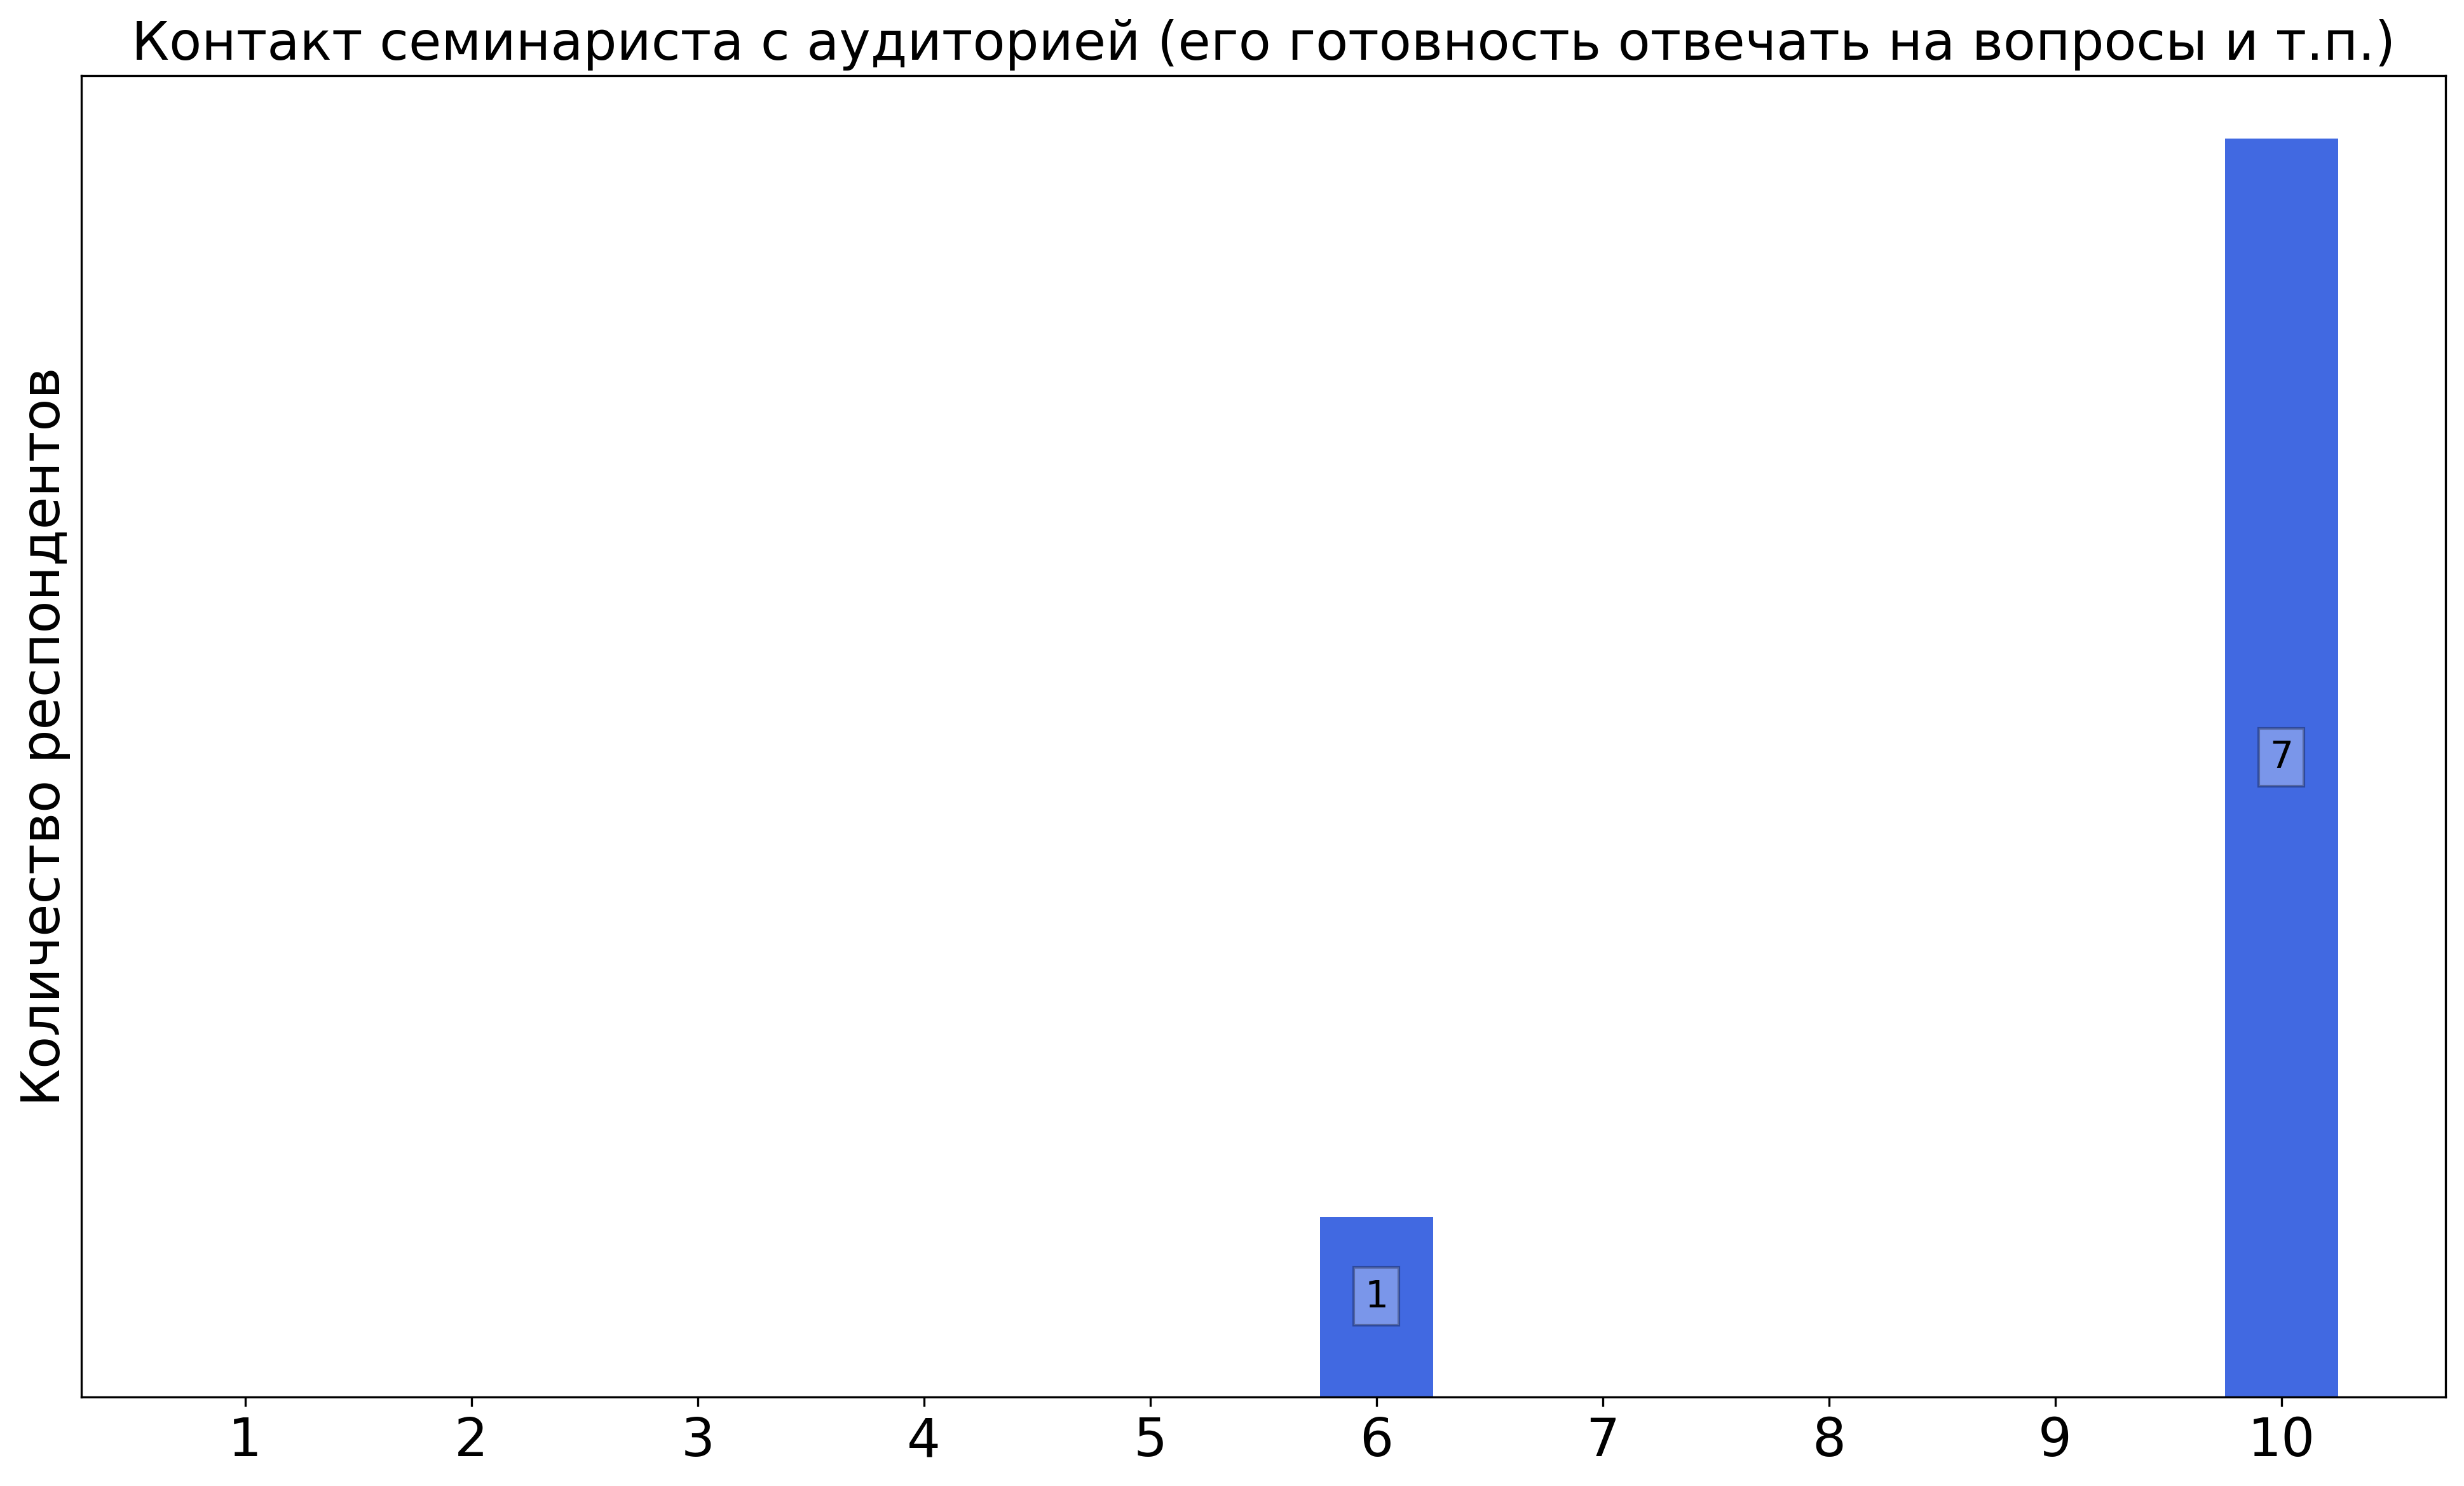
\includegraphics[width=\textwidth]{images/1 course/Аналитическая геометрия/seminarists-marks-Агаханова Я.С.-0.png}
            \end{subfigure}
            \begin{subfigure}[b]{0.45\textwidth}
                \centering
                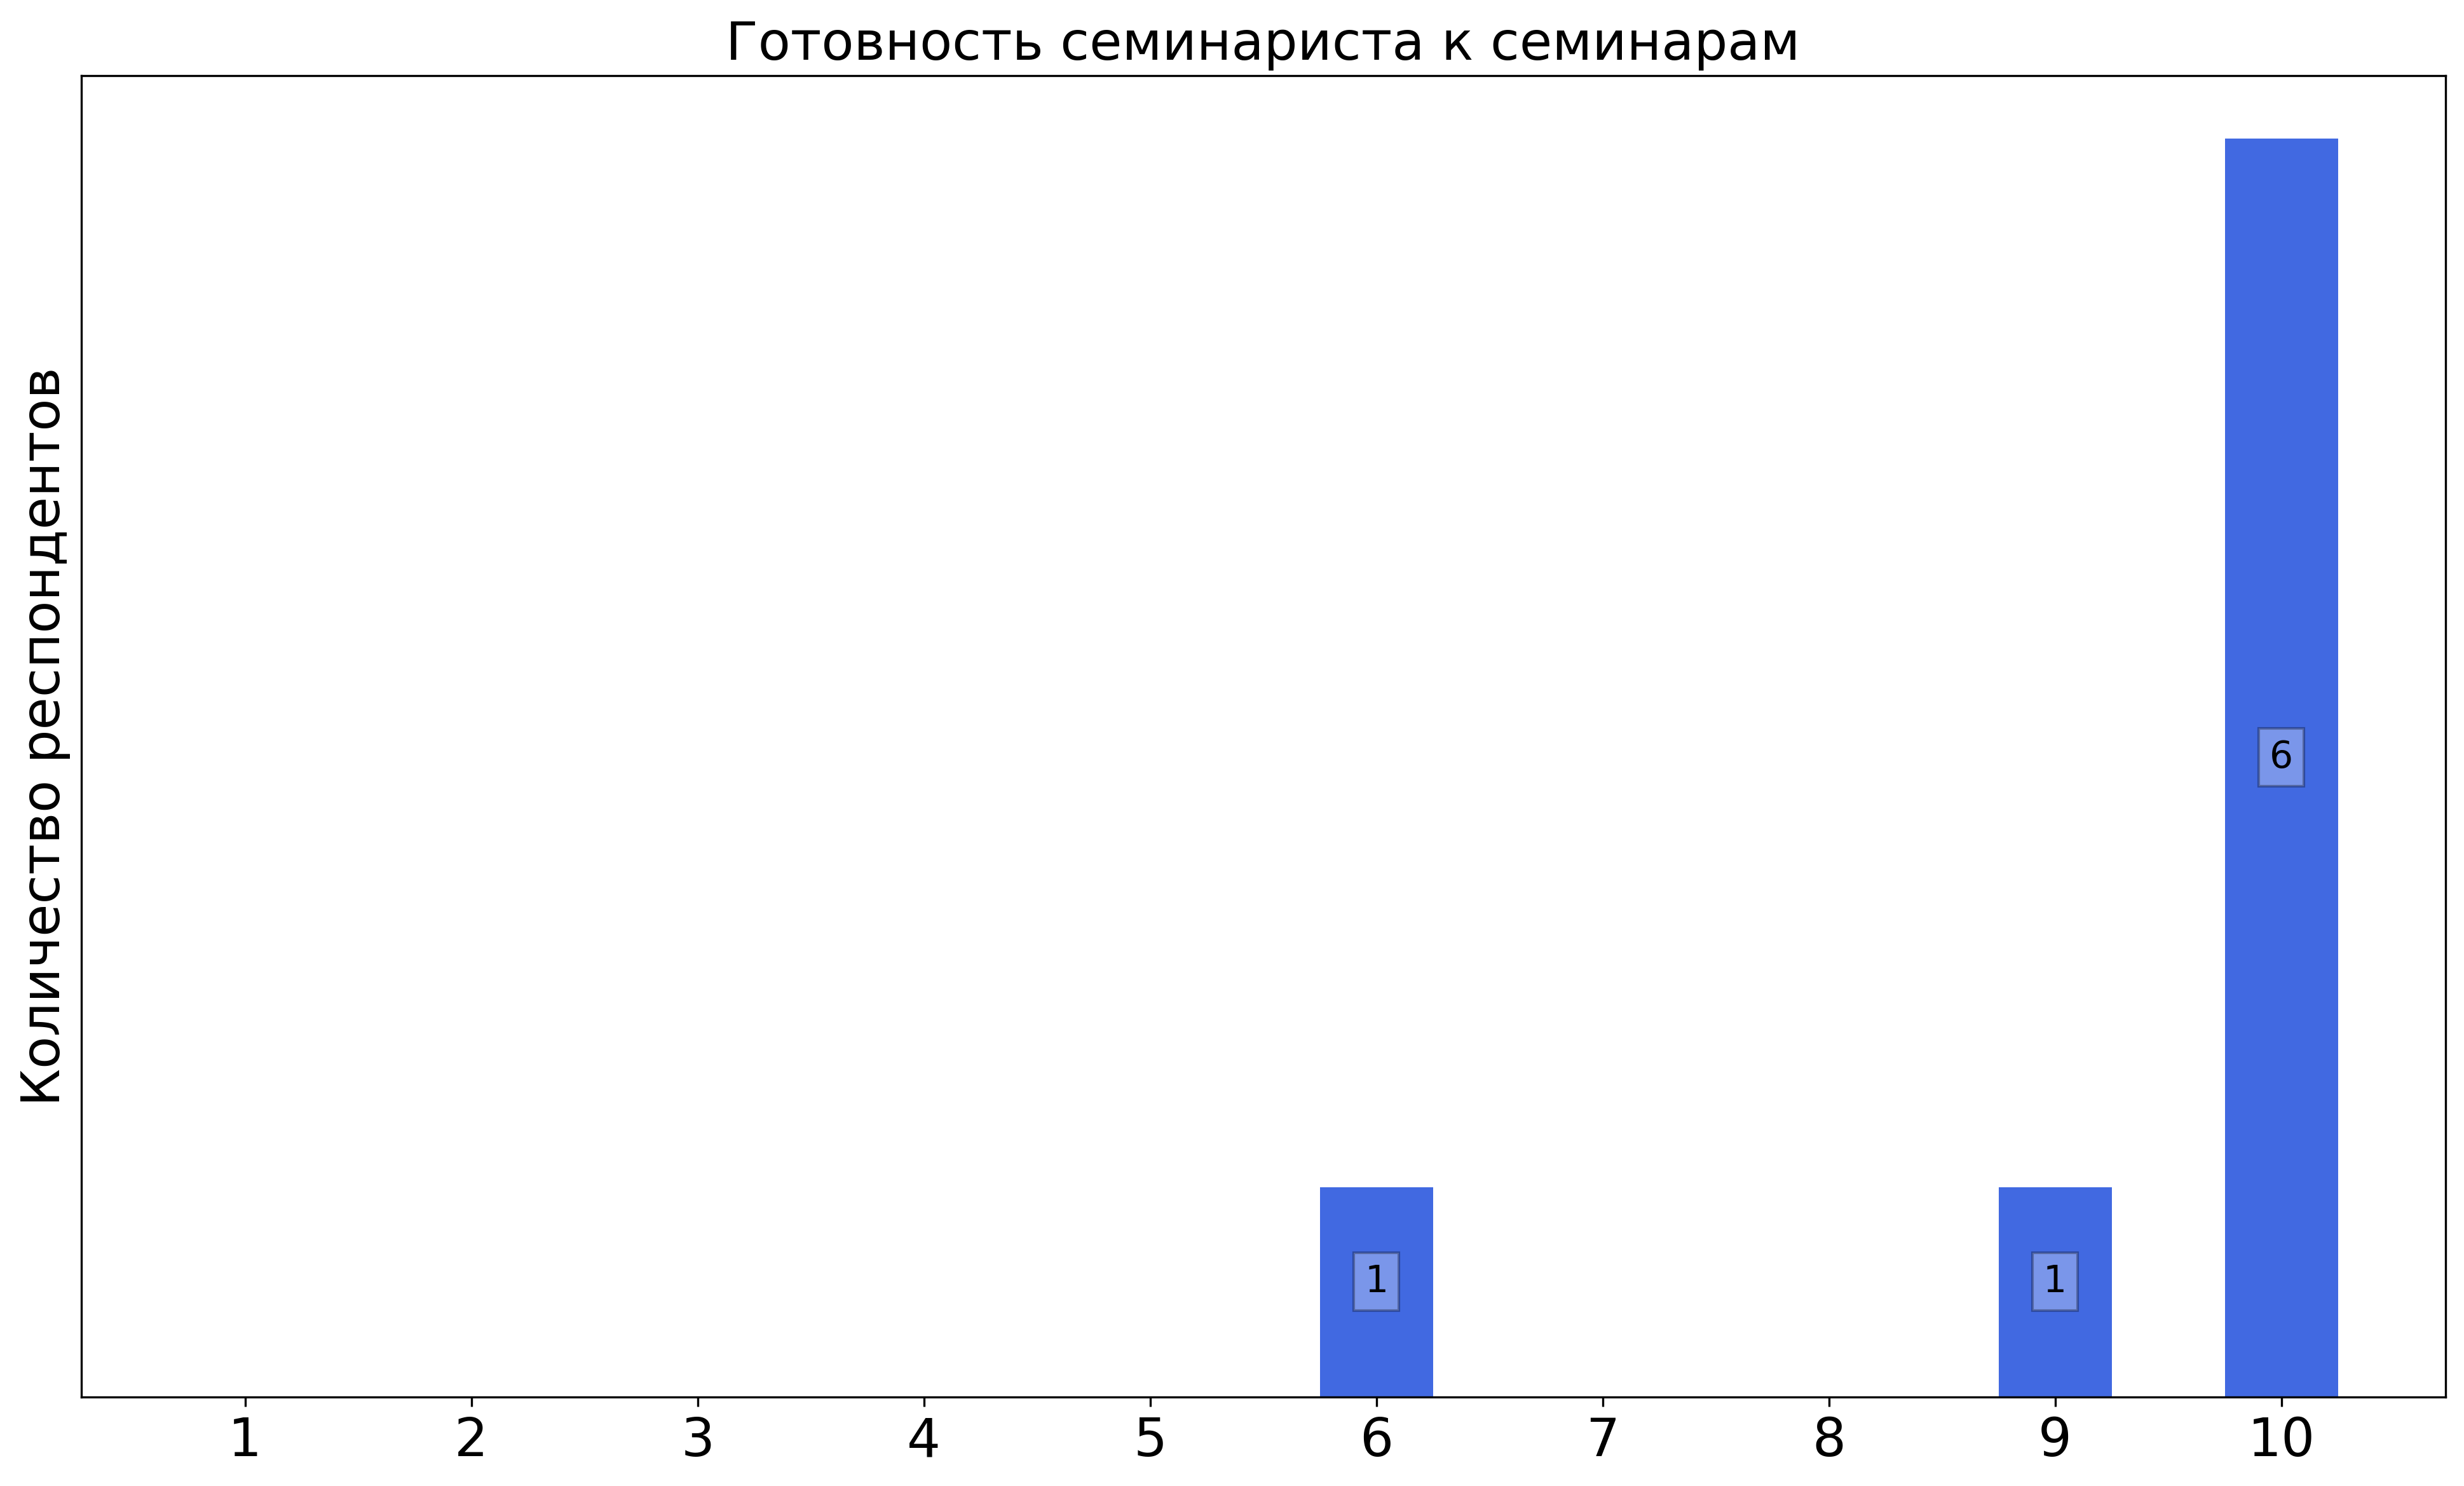
\includegraphics[width=\textwidth]{images/1 course/Аналитическая геометрия/seminarists-marks-Агаханова Я.С.-1.png}
            \end{subfigure}
            \begin{subfigure}[b]{0.45\textwidth}
                \centering
                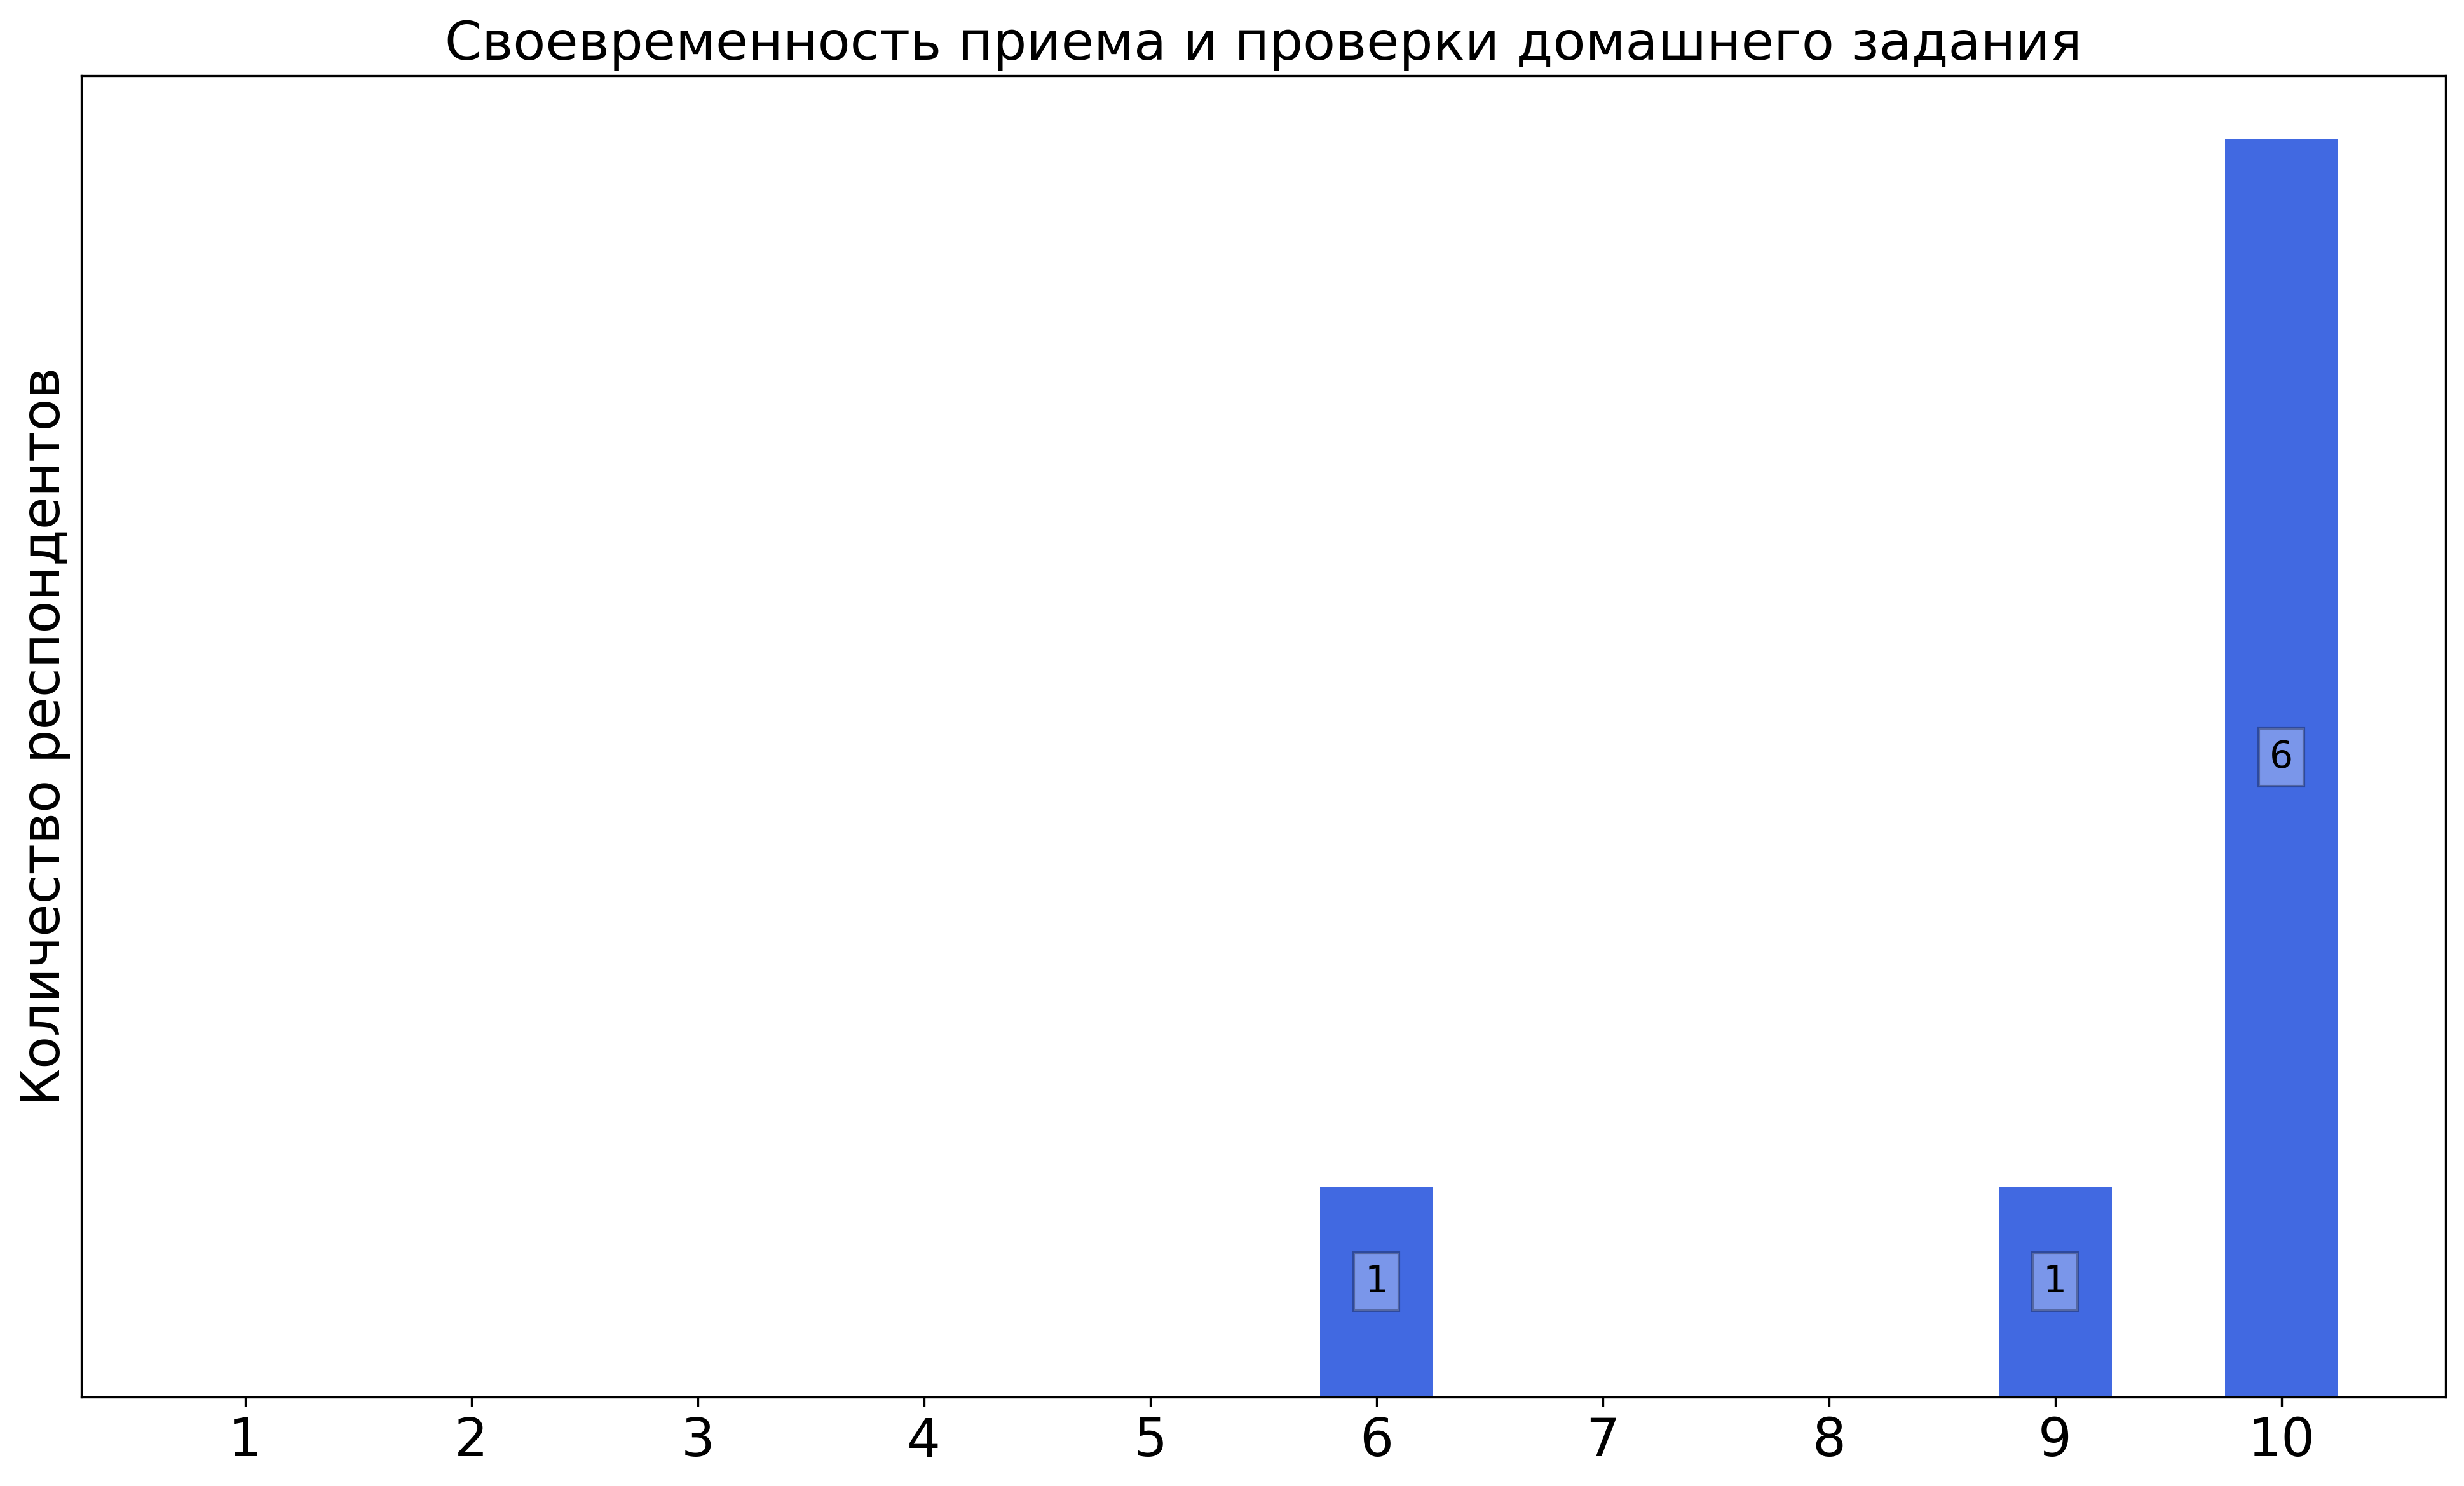
\includegraphics[width=\textwidth]{images/1 course/Аналитическая геометрия/seminarists-marks-Агаханова Я.С.-2.png}
            \end{subfigure}
            \begin{subfigure}[b]{0.45\textwidth}
                \centering
                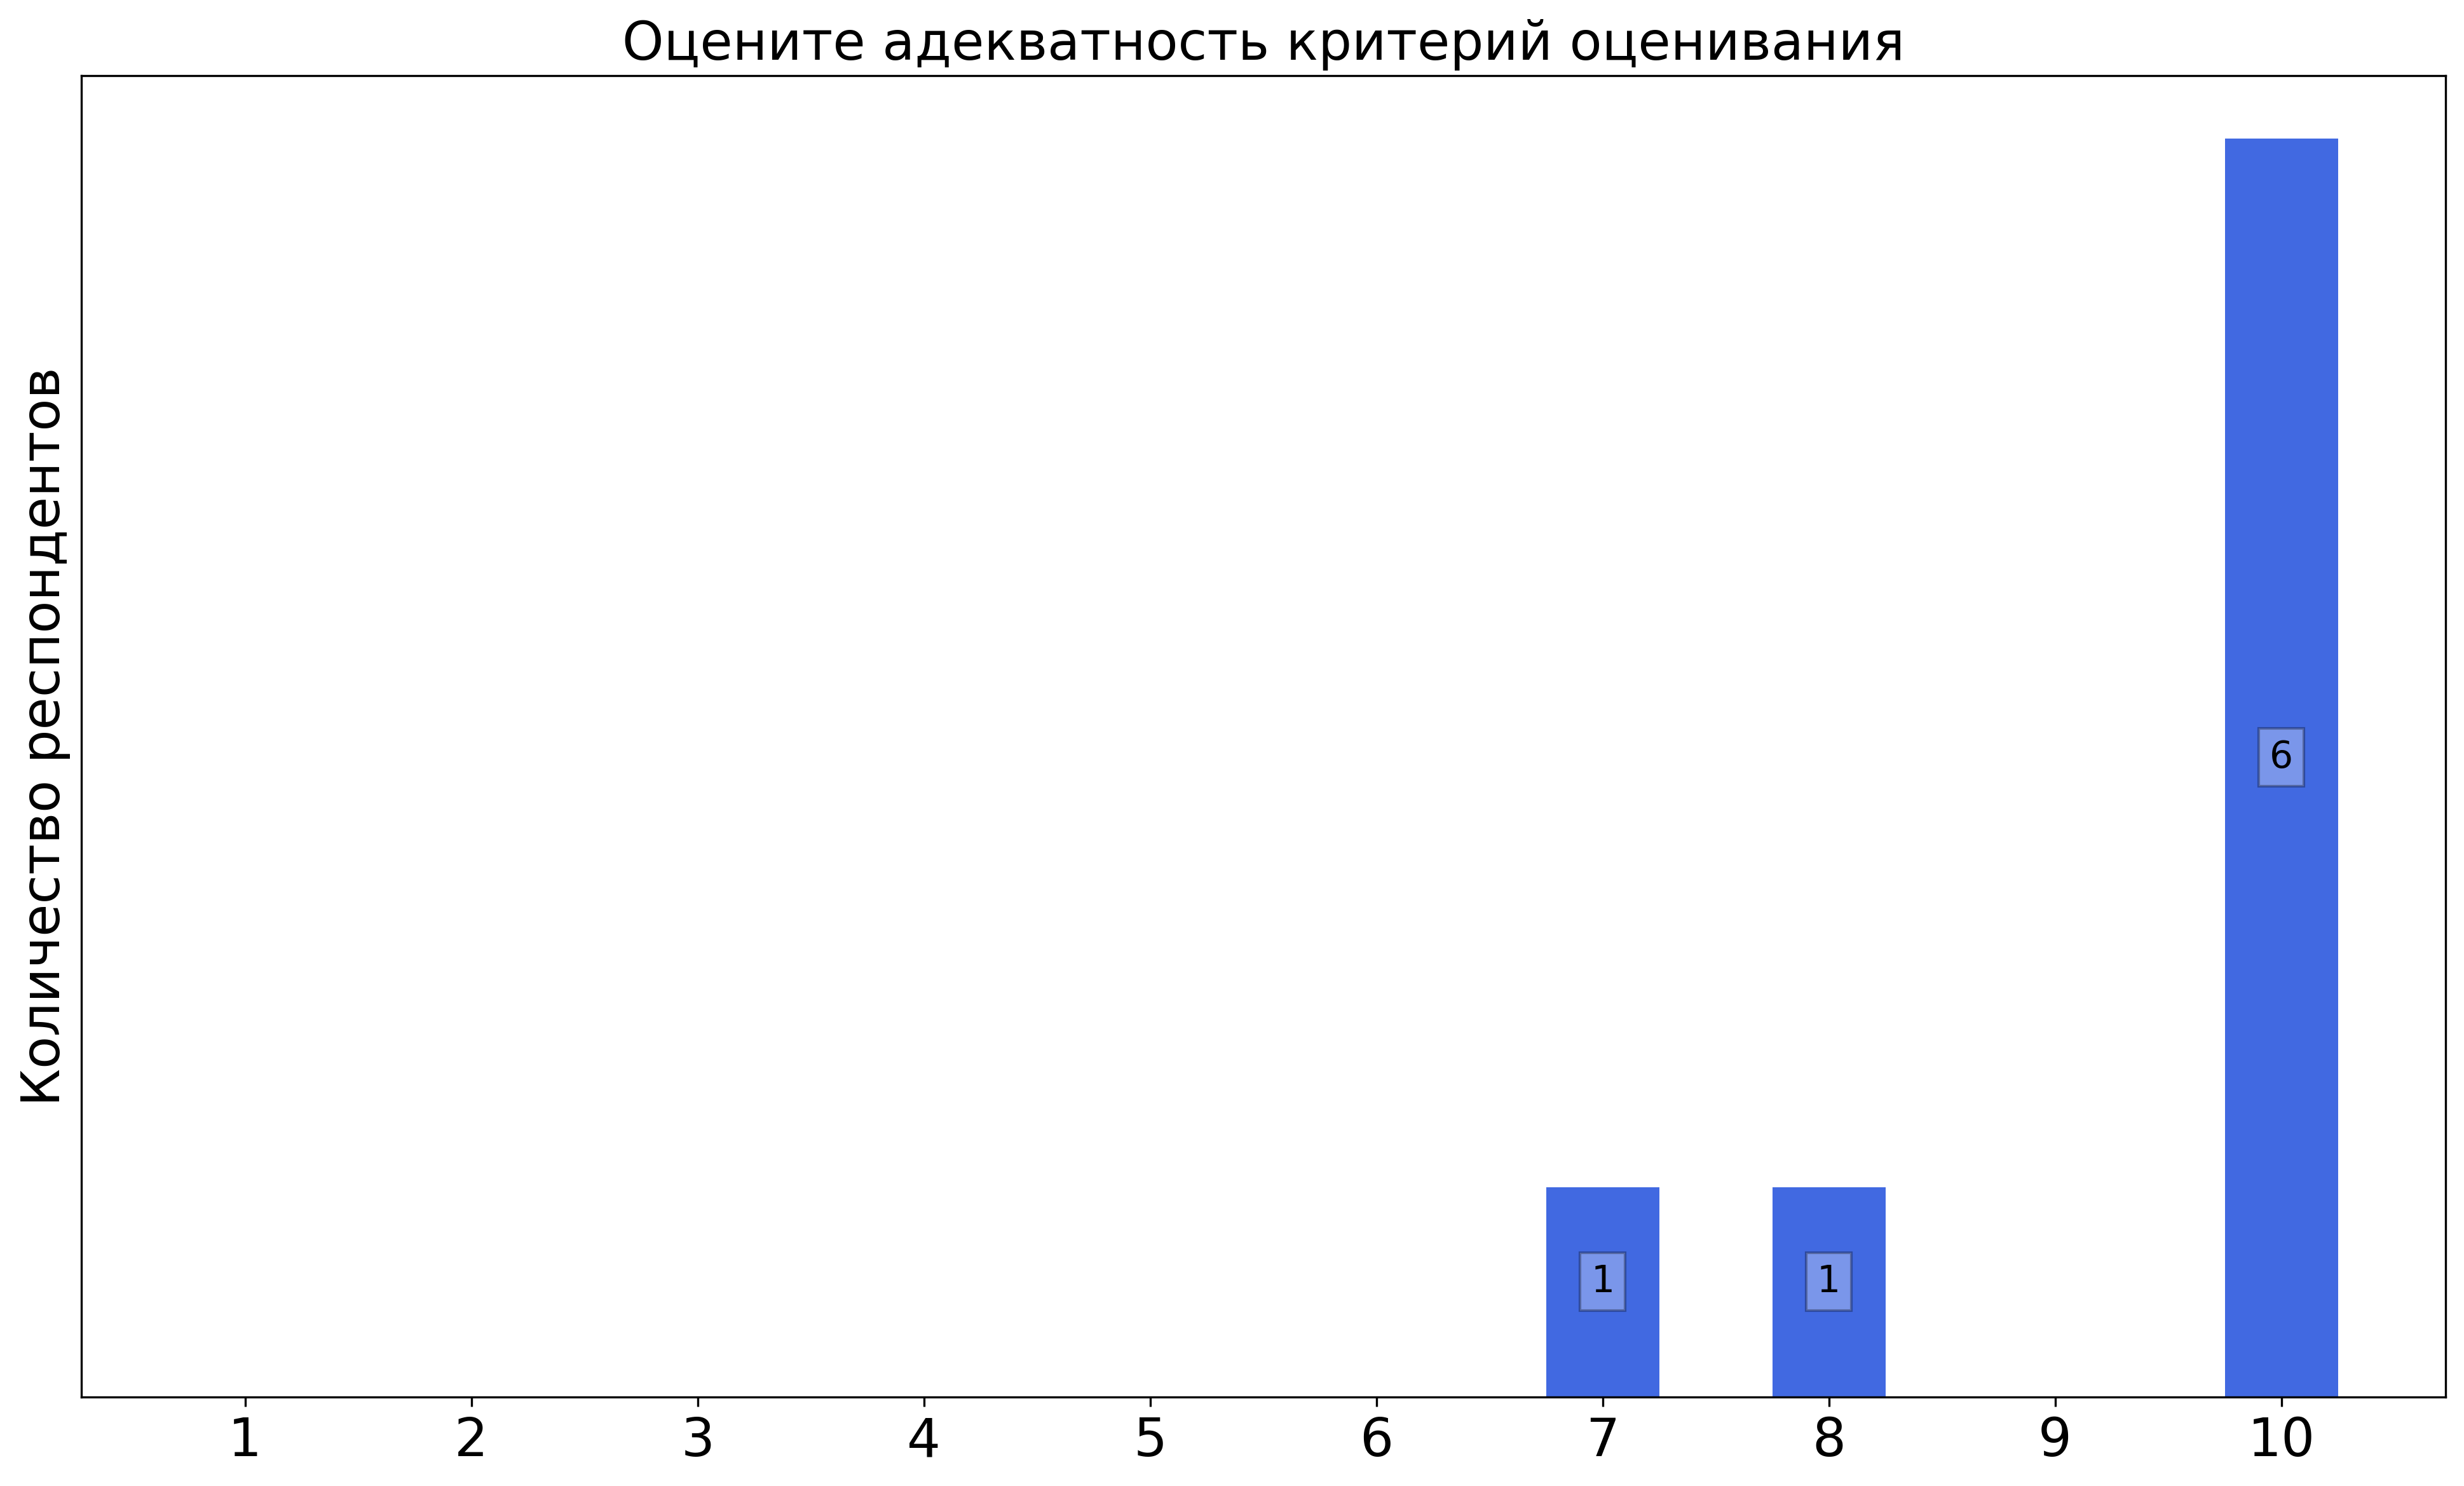
\includegraphics[width=\textwidth]{images/1 course/Аналитическая геометрия/seminarists-marks-Агаханова Я.С.-3.png}
            \end{subfigure}	
            \caption{Оценки респондентов о качестве преподавания семинаров}
        \end{figure}
    
        \textbf{Комментарии студентов о семинаристе\protect\footnote{сохранены оригинальные орфография и пунктуация}}
            \begin{commentbox} 
                Яна Сергеевна всё объясняет на пальцах, как пятиклассникам - то что и нужно 
            \end{commentbox}
            

    \subsubsection{Отзыв студентов о семинарах. Семинарист: Глухова Е.В.}
        \begin{figure}[H]
            \centering
            \begin{subfigure}[b]{0.45\textwidth}
                \centering
                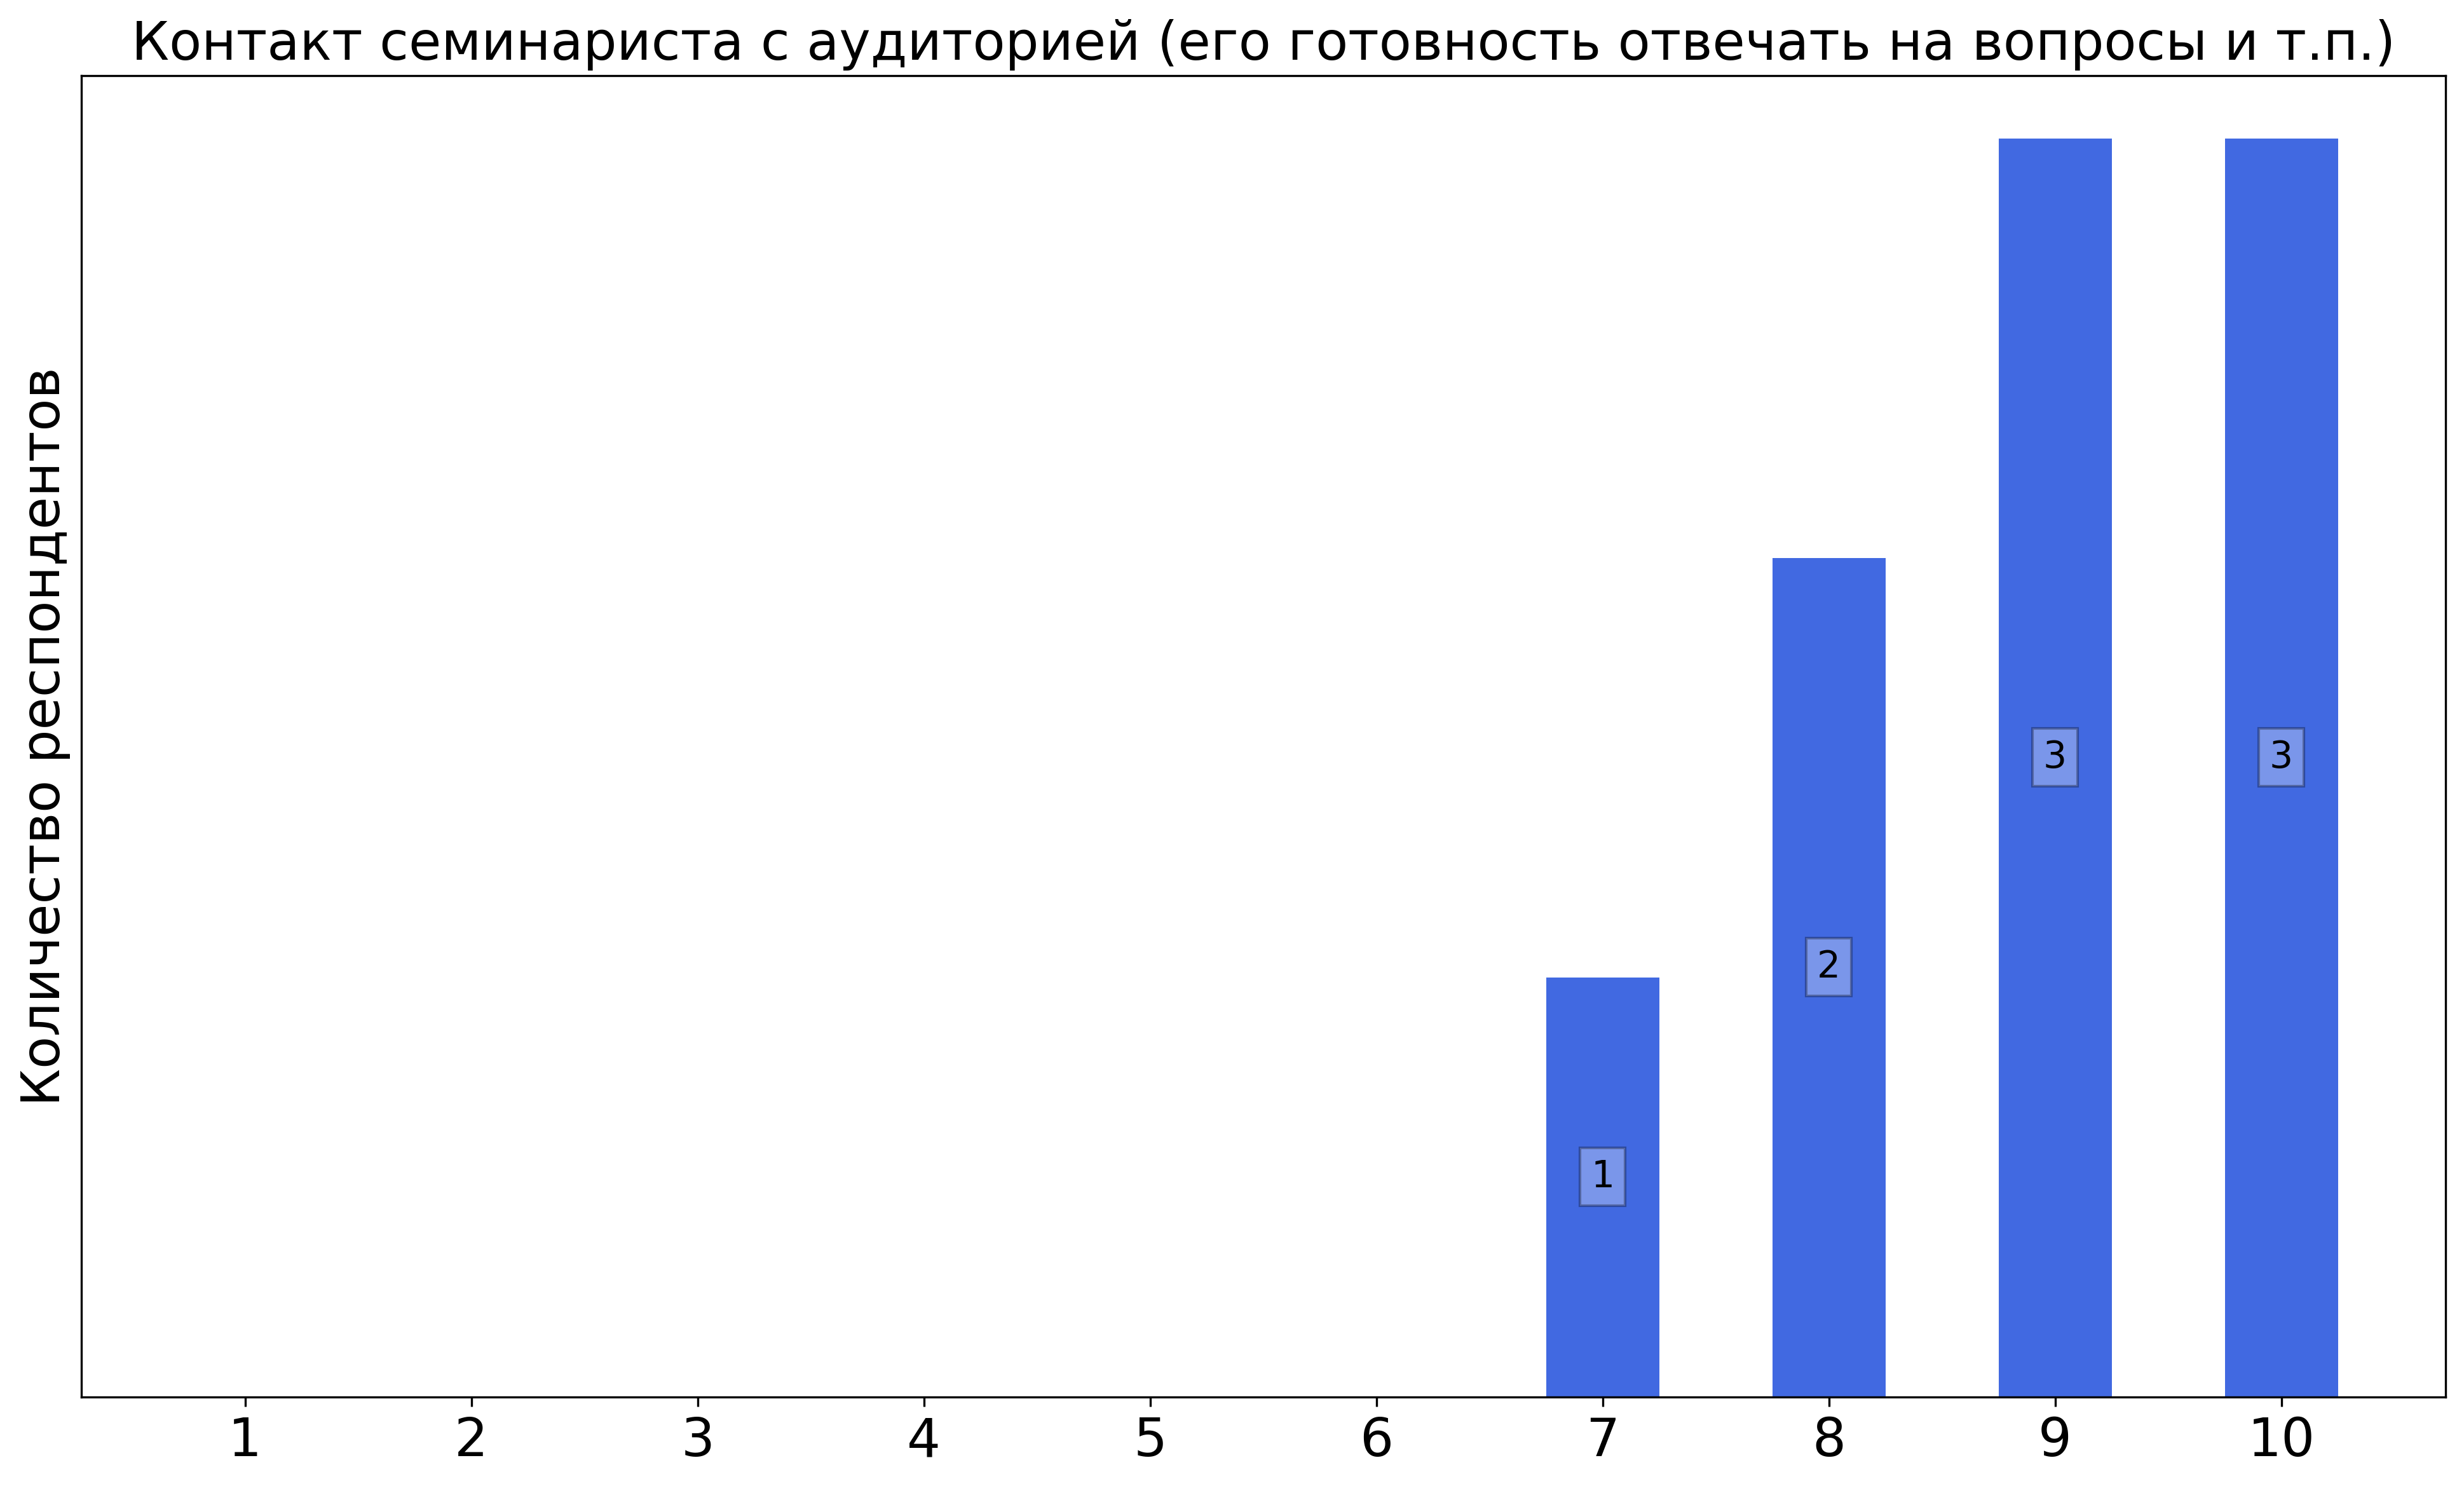
\includegraphics[width=\textwidth]{images/1 course/Аналитическая геометрия/seminarists-marks-Глухова Е.В.-0.png}
            \end{subfigure}
            \begin{subfigure}[b]{0.45\textwidth}
                \centering
                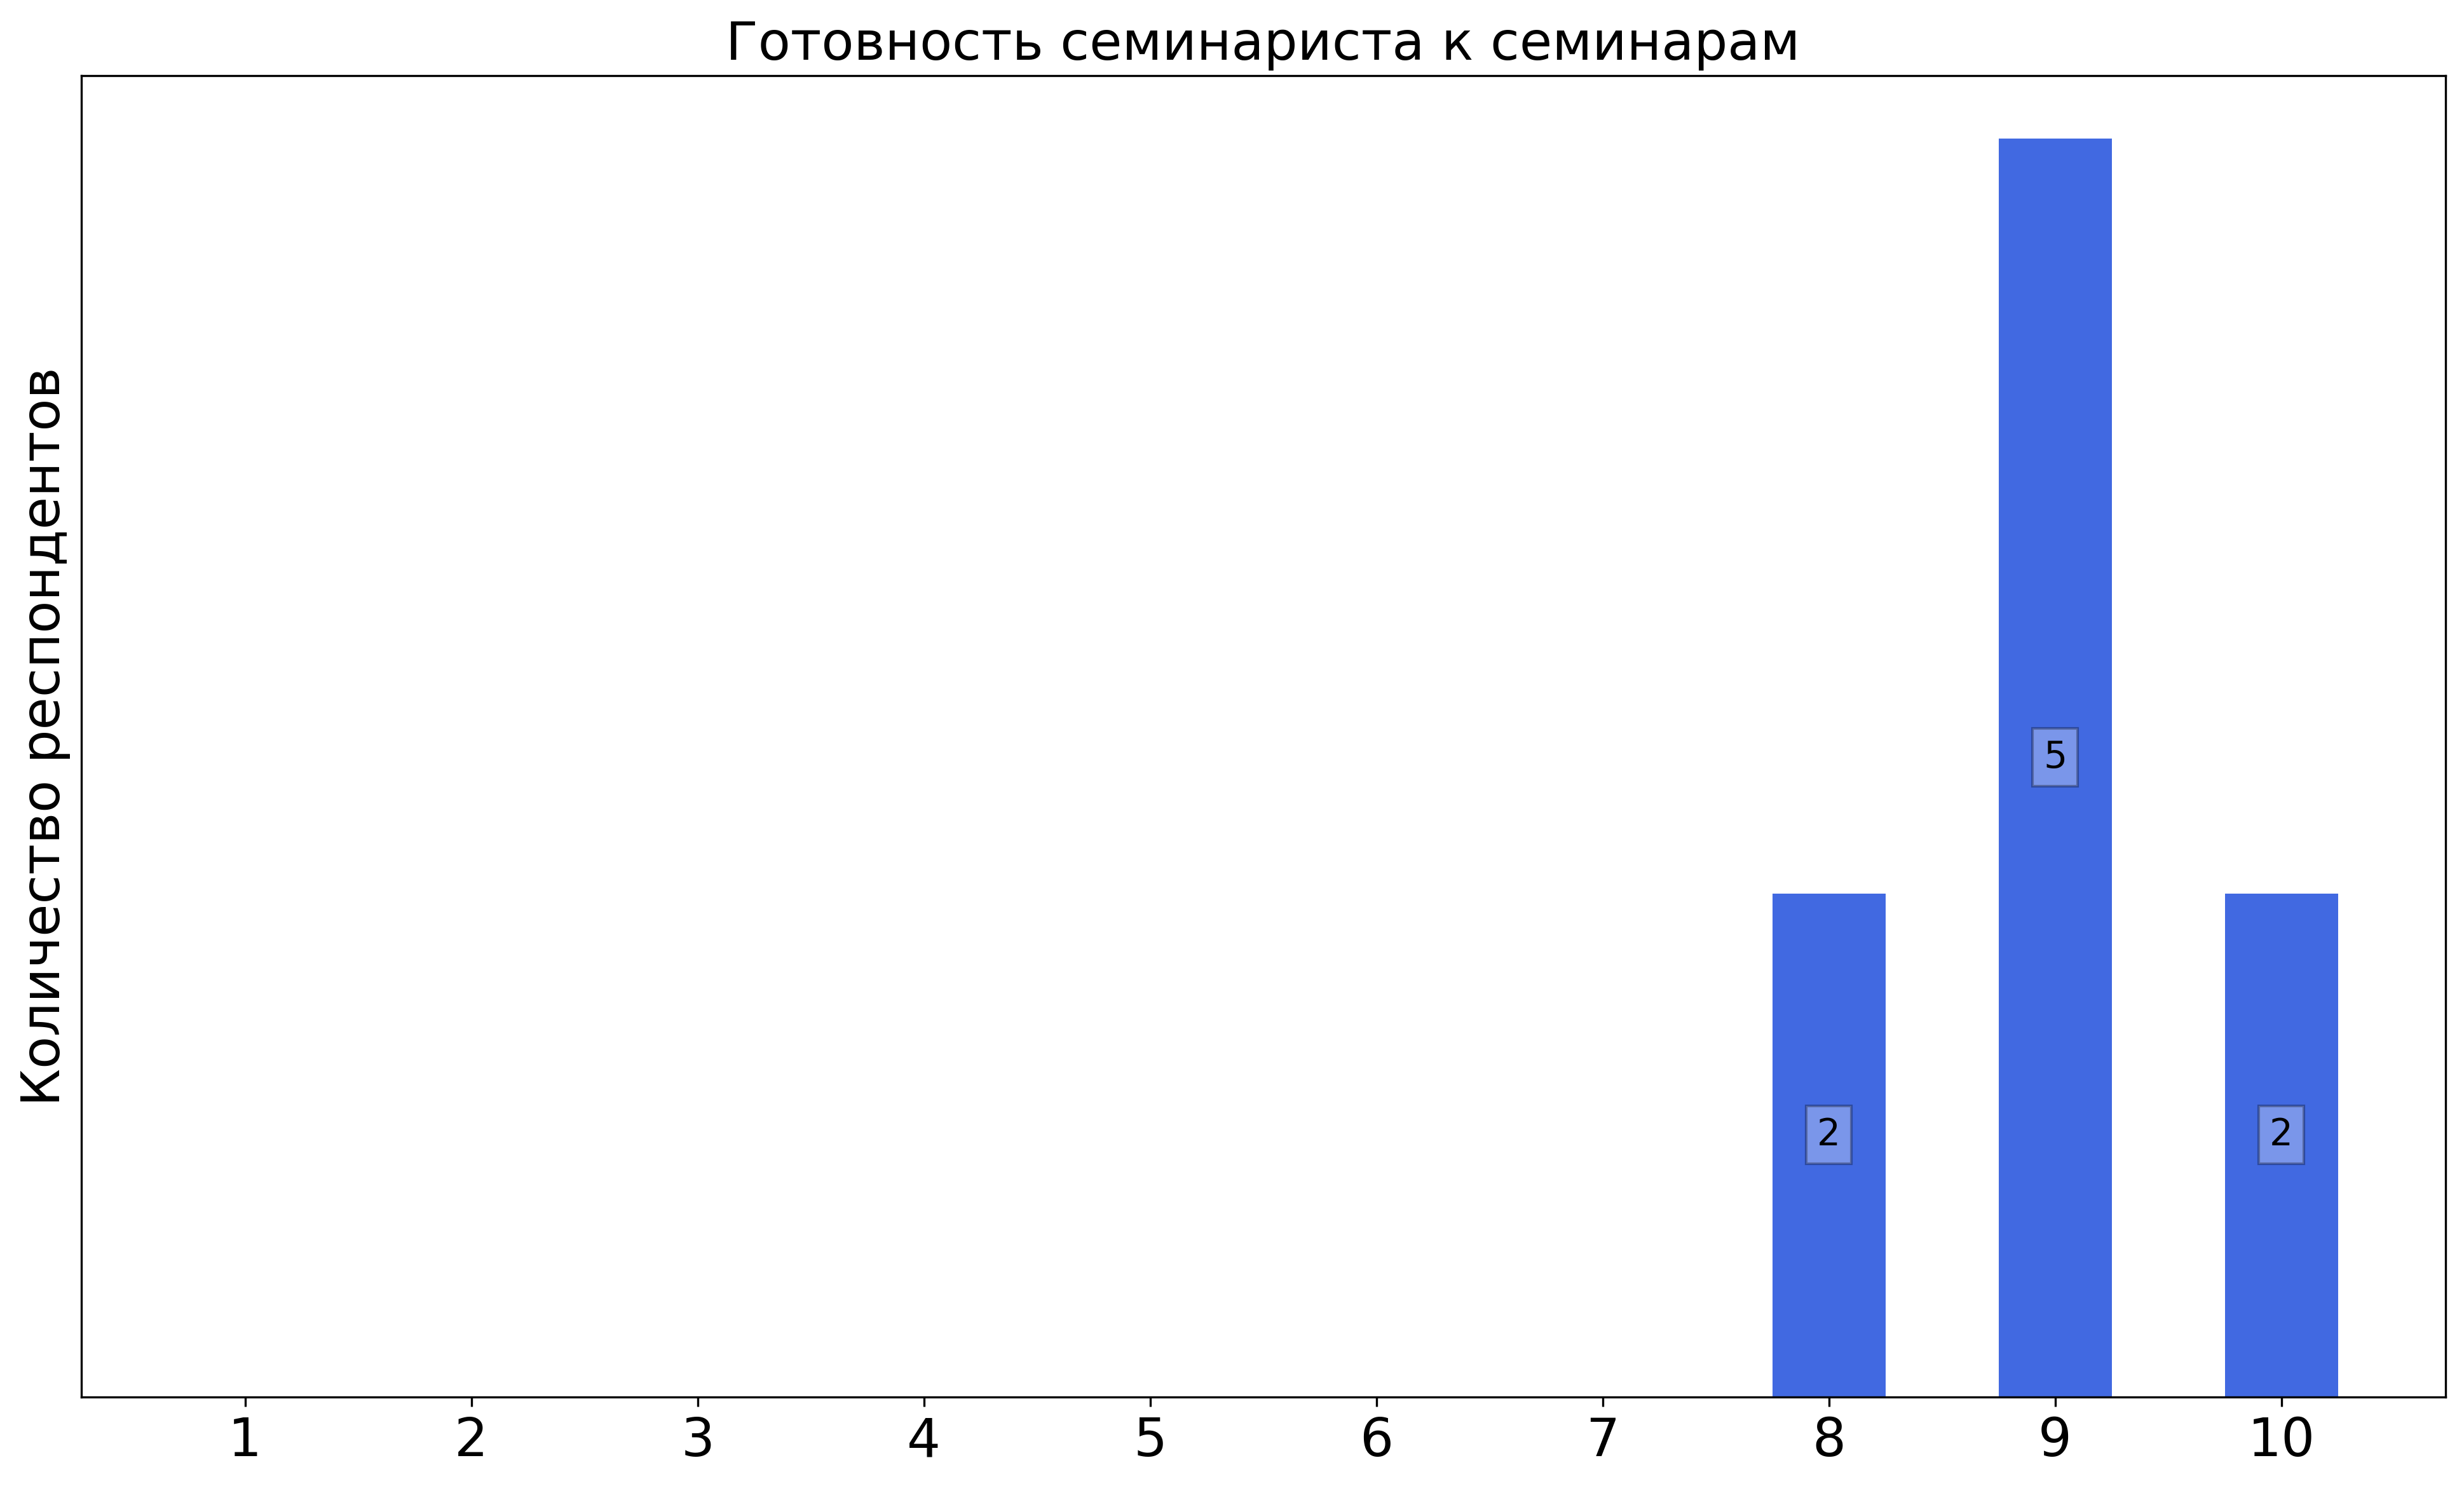
\includegraphics[width=\textwidth]{images/1 course/Аналитическая геометрия/seminarists-marks-Глухова Е.В.-1.png}
            \end{subfigure}
            \begin{subfigure}[b]{0.45\textwidth}
                \centering
                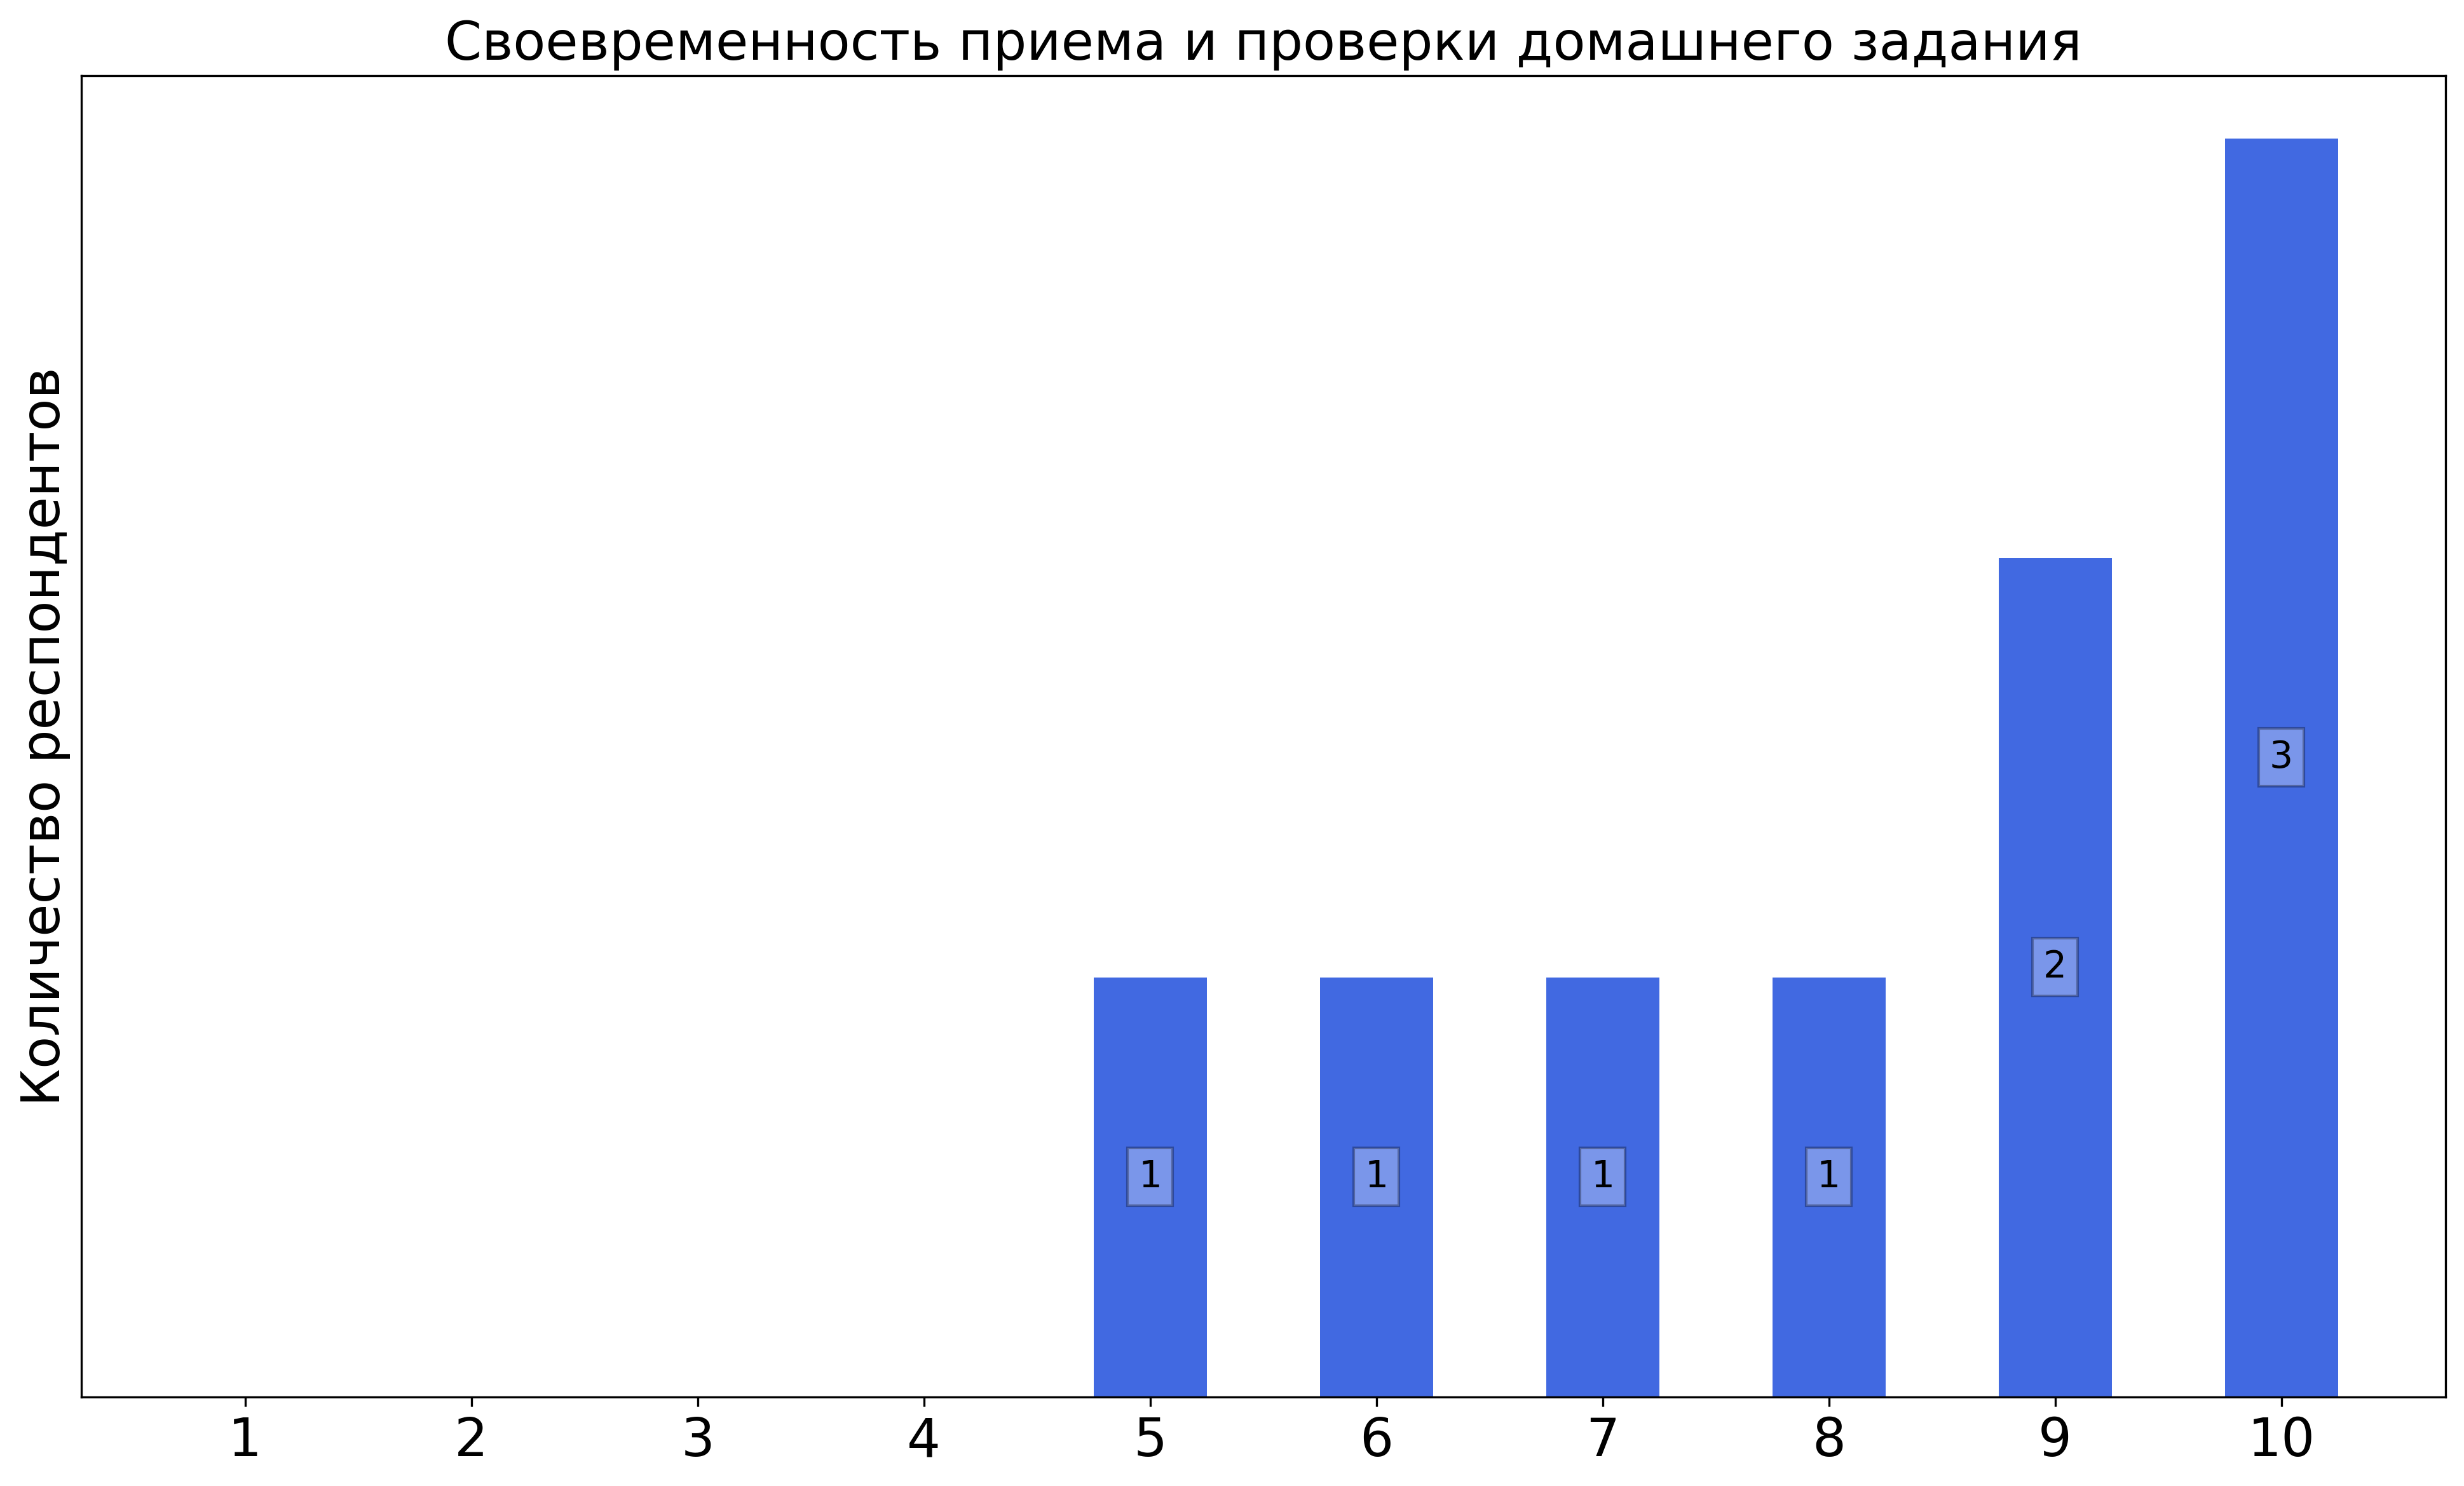
\includegraphics[width=\textwidth]{images/1 course/Аналитическая геометрия/seminarists-marks-Глухова Е.В.-2.png}
            \end{subfigure}
            \begin{subfigure}[b]{0.45\textwidth}
                \centering
                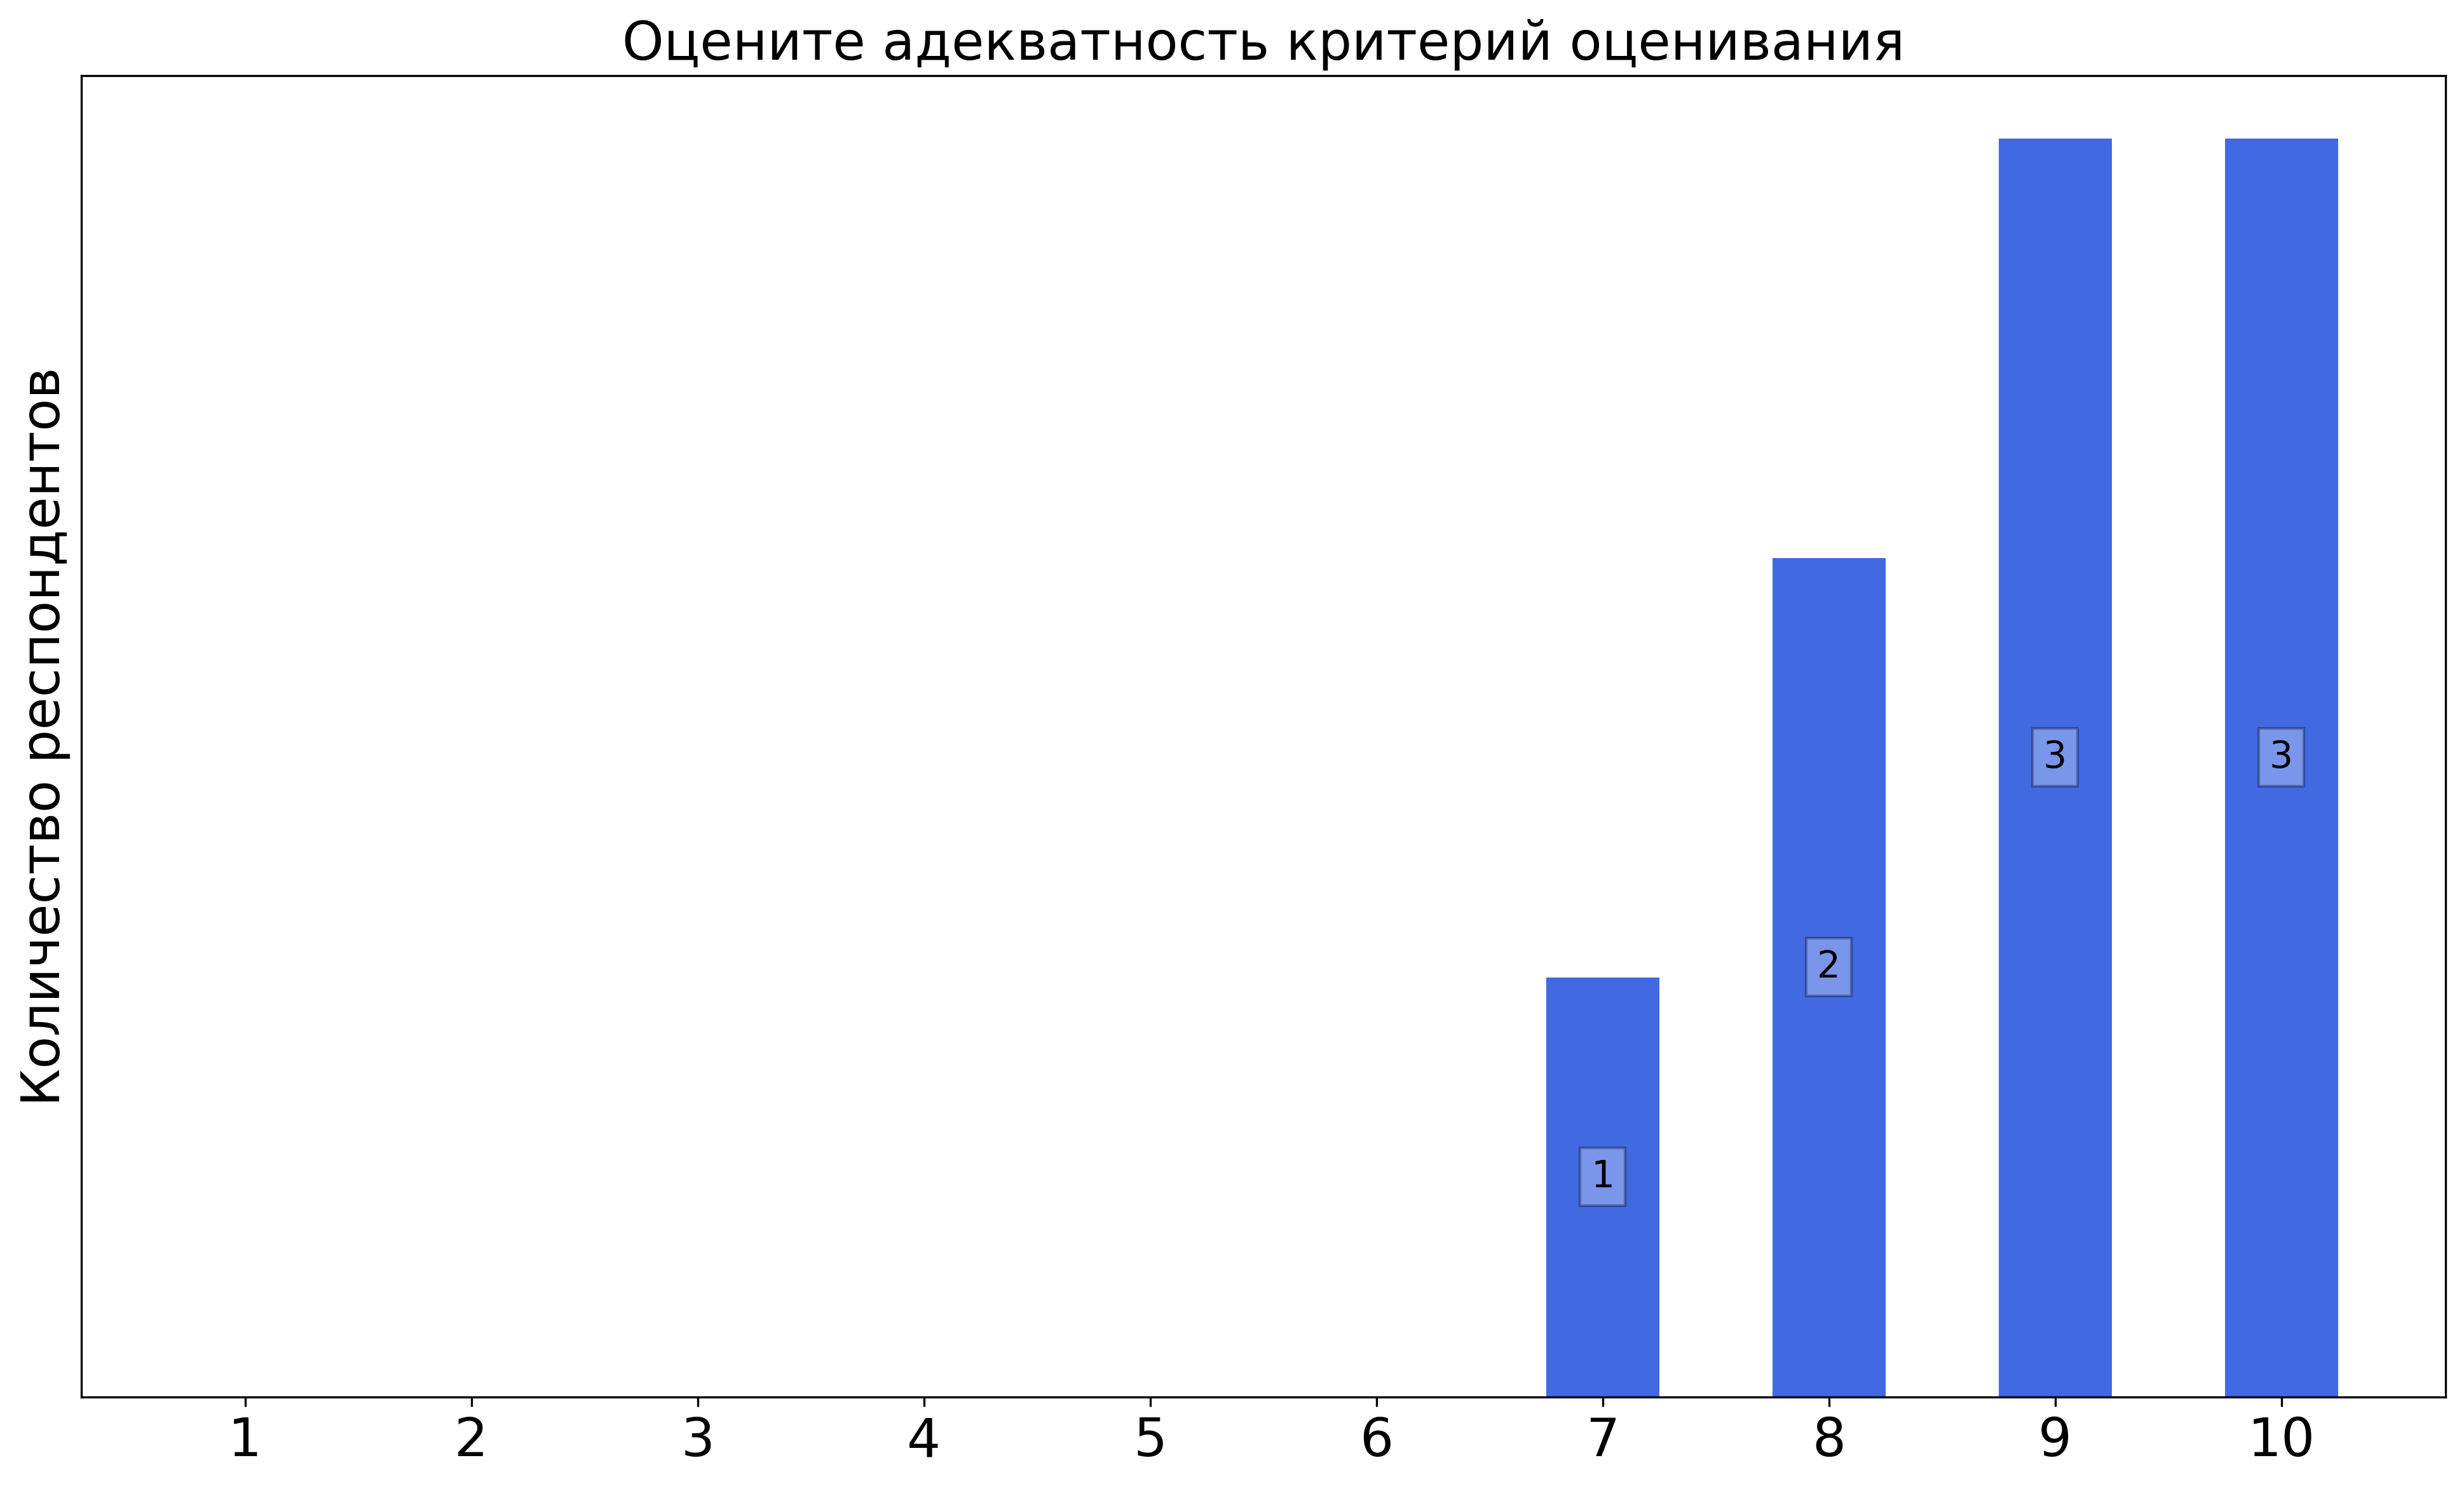
\includegraphics[width=\textwidth]{images/1 course/Аналитическая геометрия/seminarists-marks-Глухова Е.В.-3.png}
            \end{subfigure}	
            \caption{Оценки респондентов о качестве преподавания семинаров}
        \end{figure}

        \textbf{Комментарии студентов о семинаристе\protect\footnote{сохранены оригинальные орфография и пунктуация}}
            \begin{commentbox} 
                Вообще нет минусов, лишь много тратив времени на то, чтобы похвалить себя саму 
            \end{commentbox} 
        
            \begin{commentbox} 
                Очень легко забывается и начинает говорить о жизни на семинарах, а потом начинает подгонять и говорить, что ничего не успеваем, вследствие этого некоторые задачи рассматриваются очень поверхностно 
            \end{commentbox}

    \subsubsection{Отзыв студентов о семинарах. Семинарист: Петрович А.А.}
        \begin{figure}[H]
            \centering
            \begin{subfigure}[b]{0.45\textwidth}
                \centering
                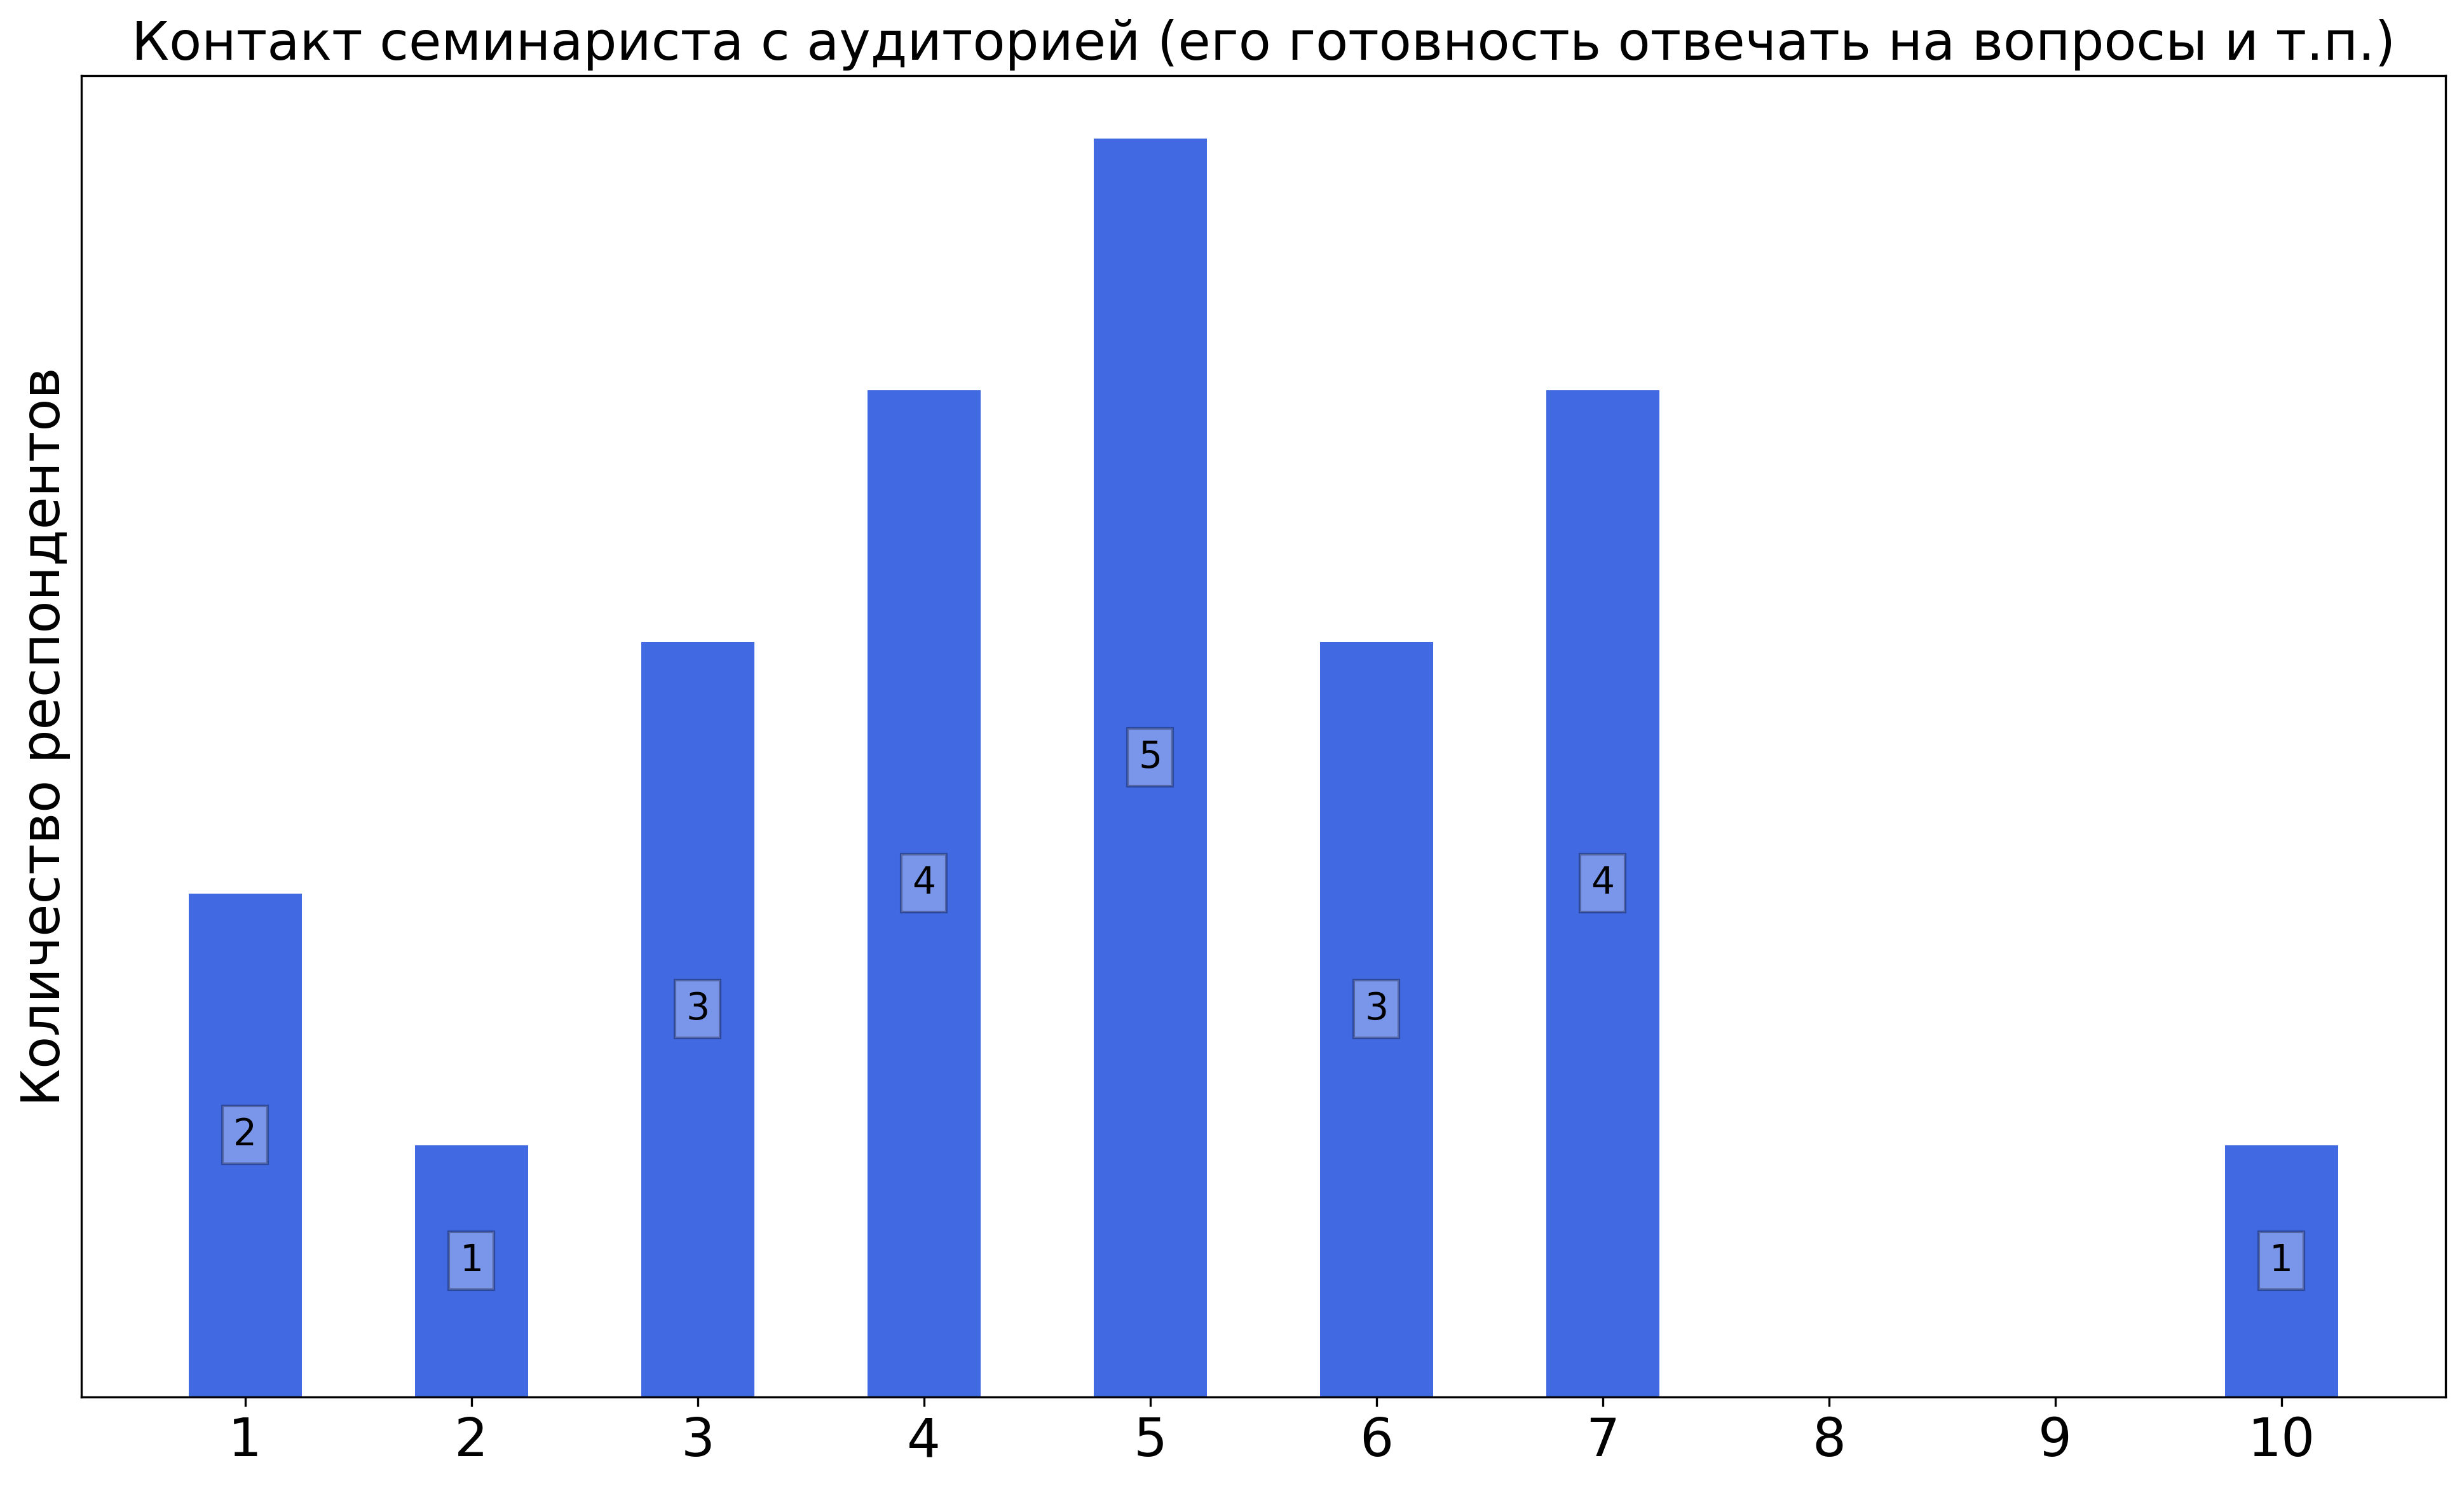
\includegraphics[width=\textwidth]{images/1 course/Аналитическая геометрия/seminarists-marks-Петрович А.А.-0.png}
            \end{subfigure}
            \begin{subfigure}[b]{0.45\textwidth}
                \centering
                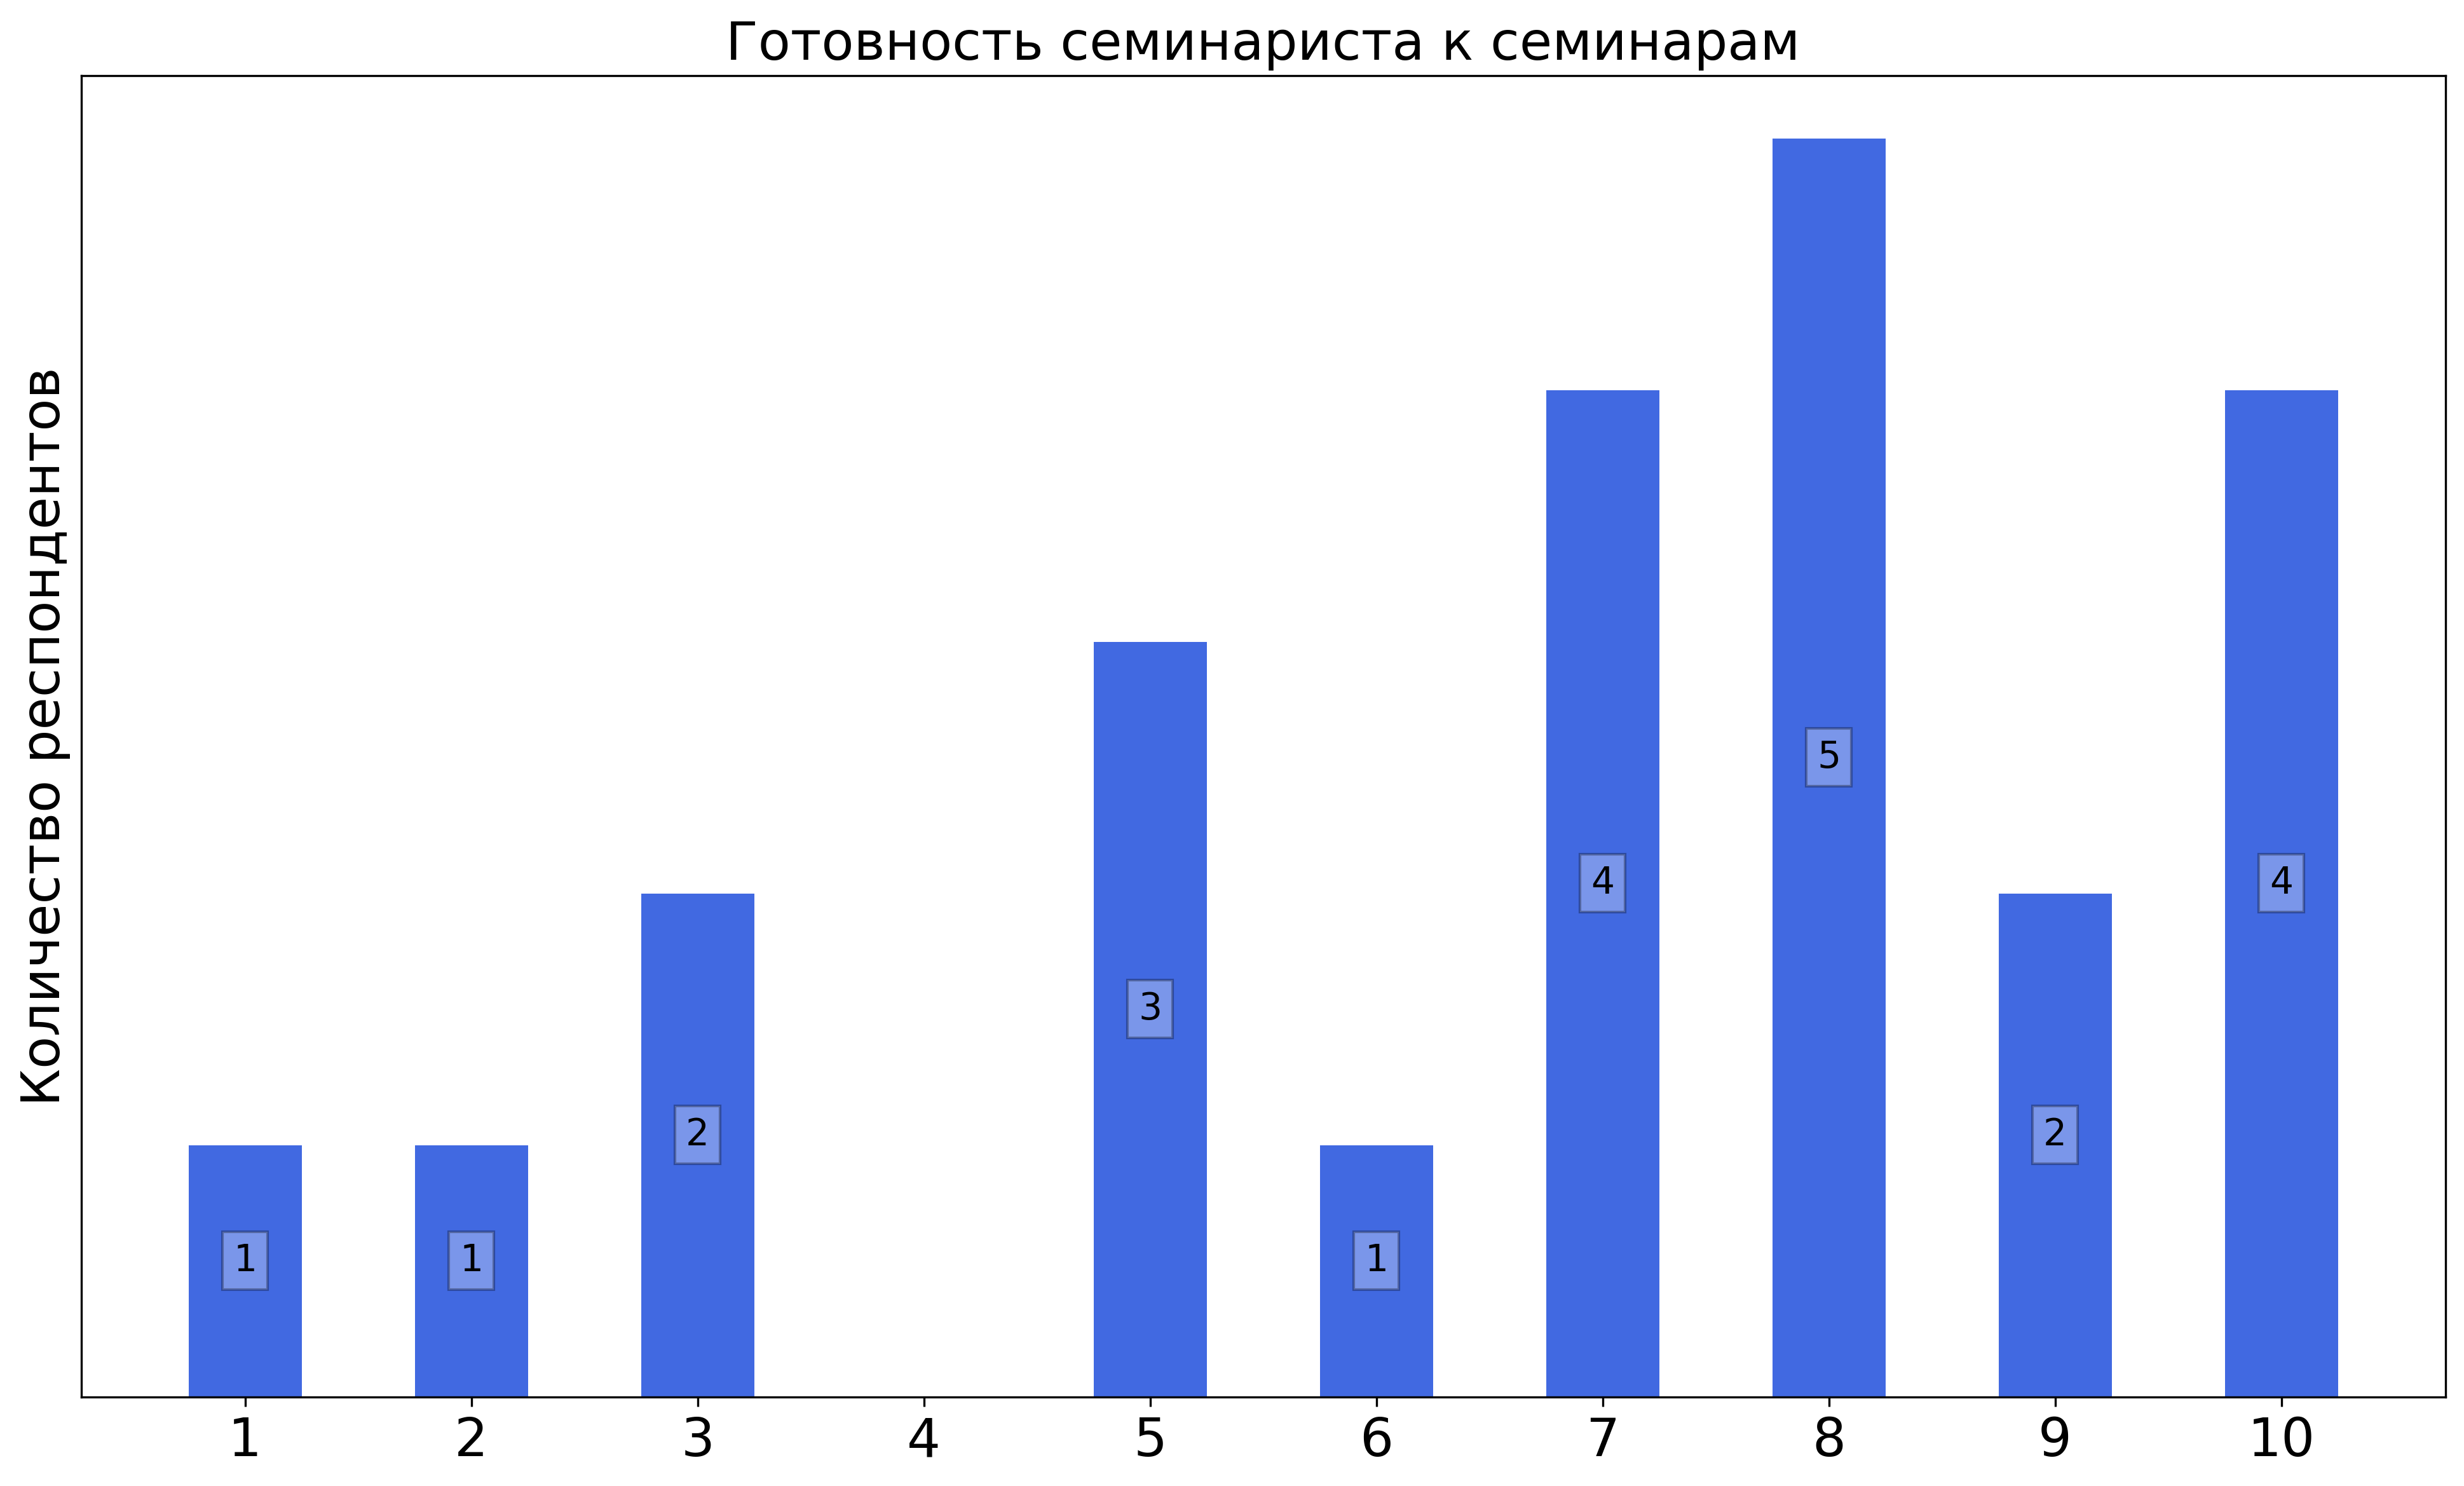
\includegraphics[width=\textwidth]{images/1 course/Аналитическая геометрия/seminarists-marks-Петрович А.А.-1.png}
            \end{subfigure}
            \begin{subfigure}[b]{0.45\textwidth}
                \centering
                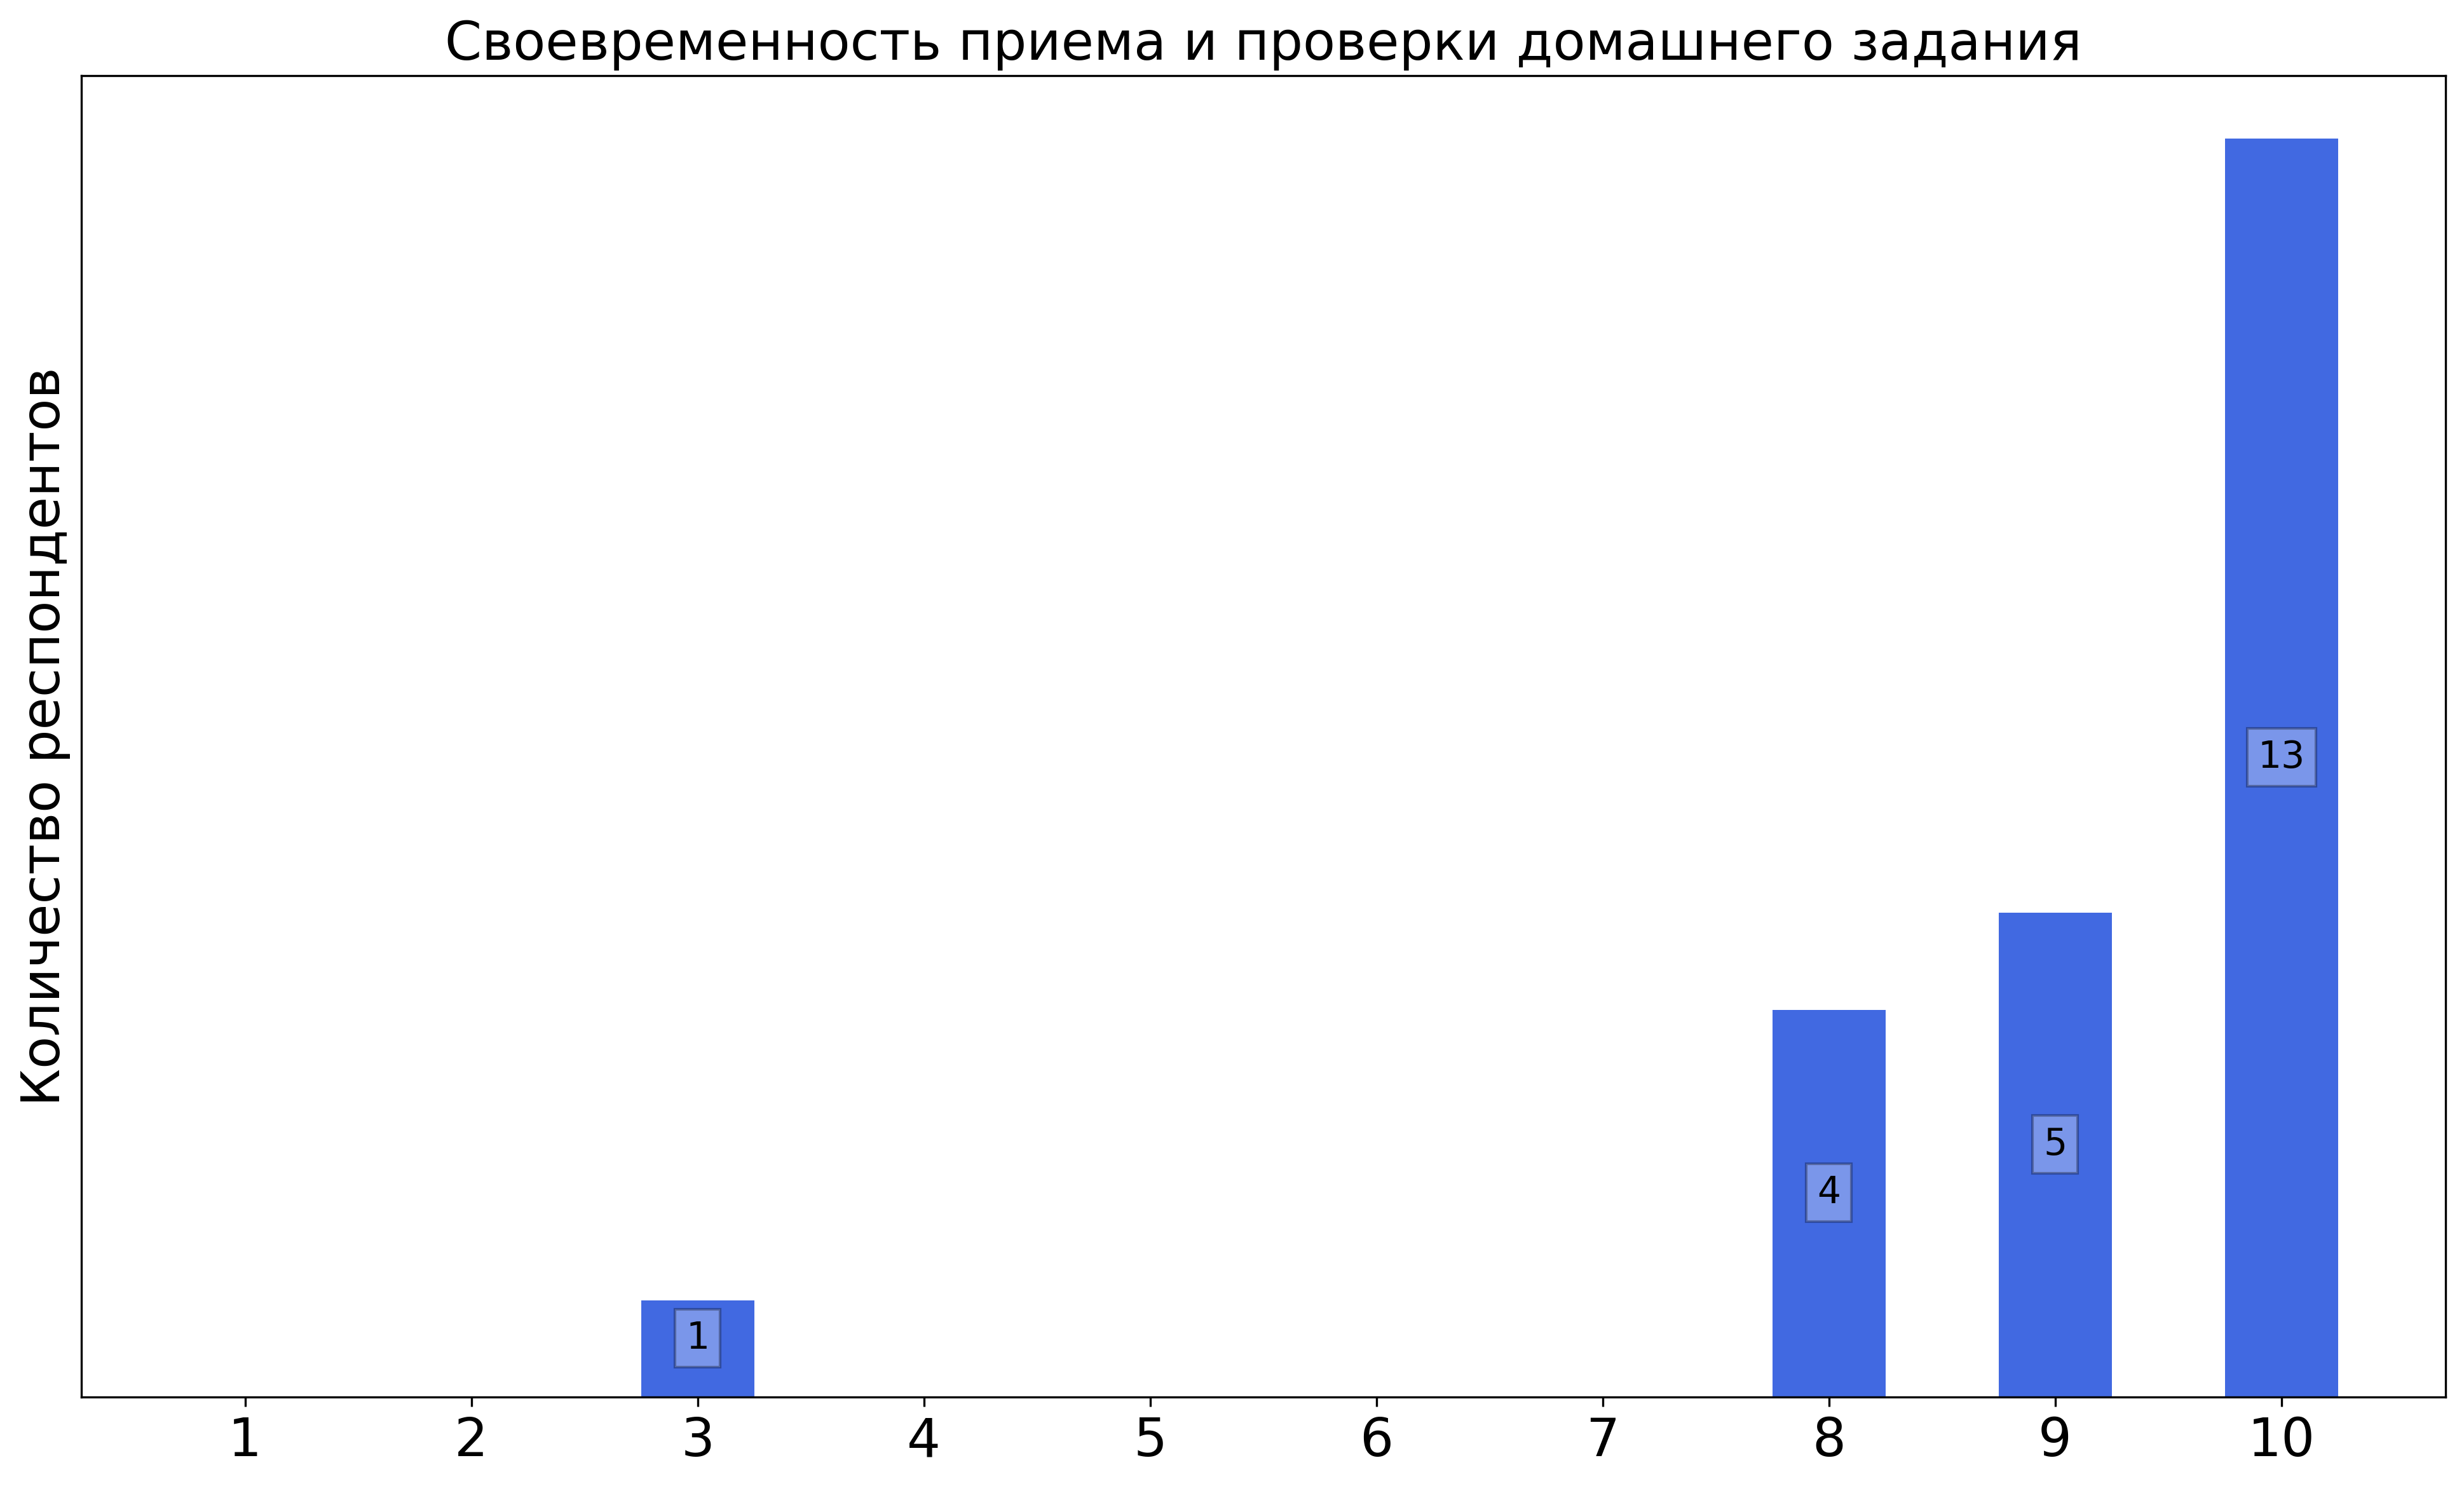
\includegraphics[width=\textwidth]{images/1 course/Аналитическая геометрия/seminarists-marks-Петрович А.А.-2.png}
            \end{subfigure}
            \begin{subfigure}[b]{0.45\textwidth}
                \centering
                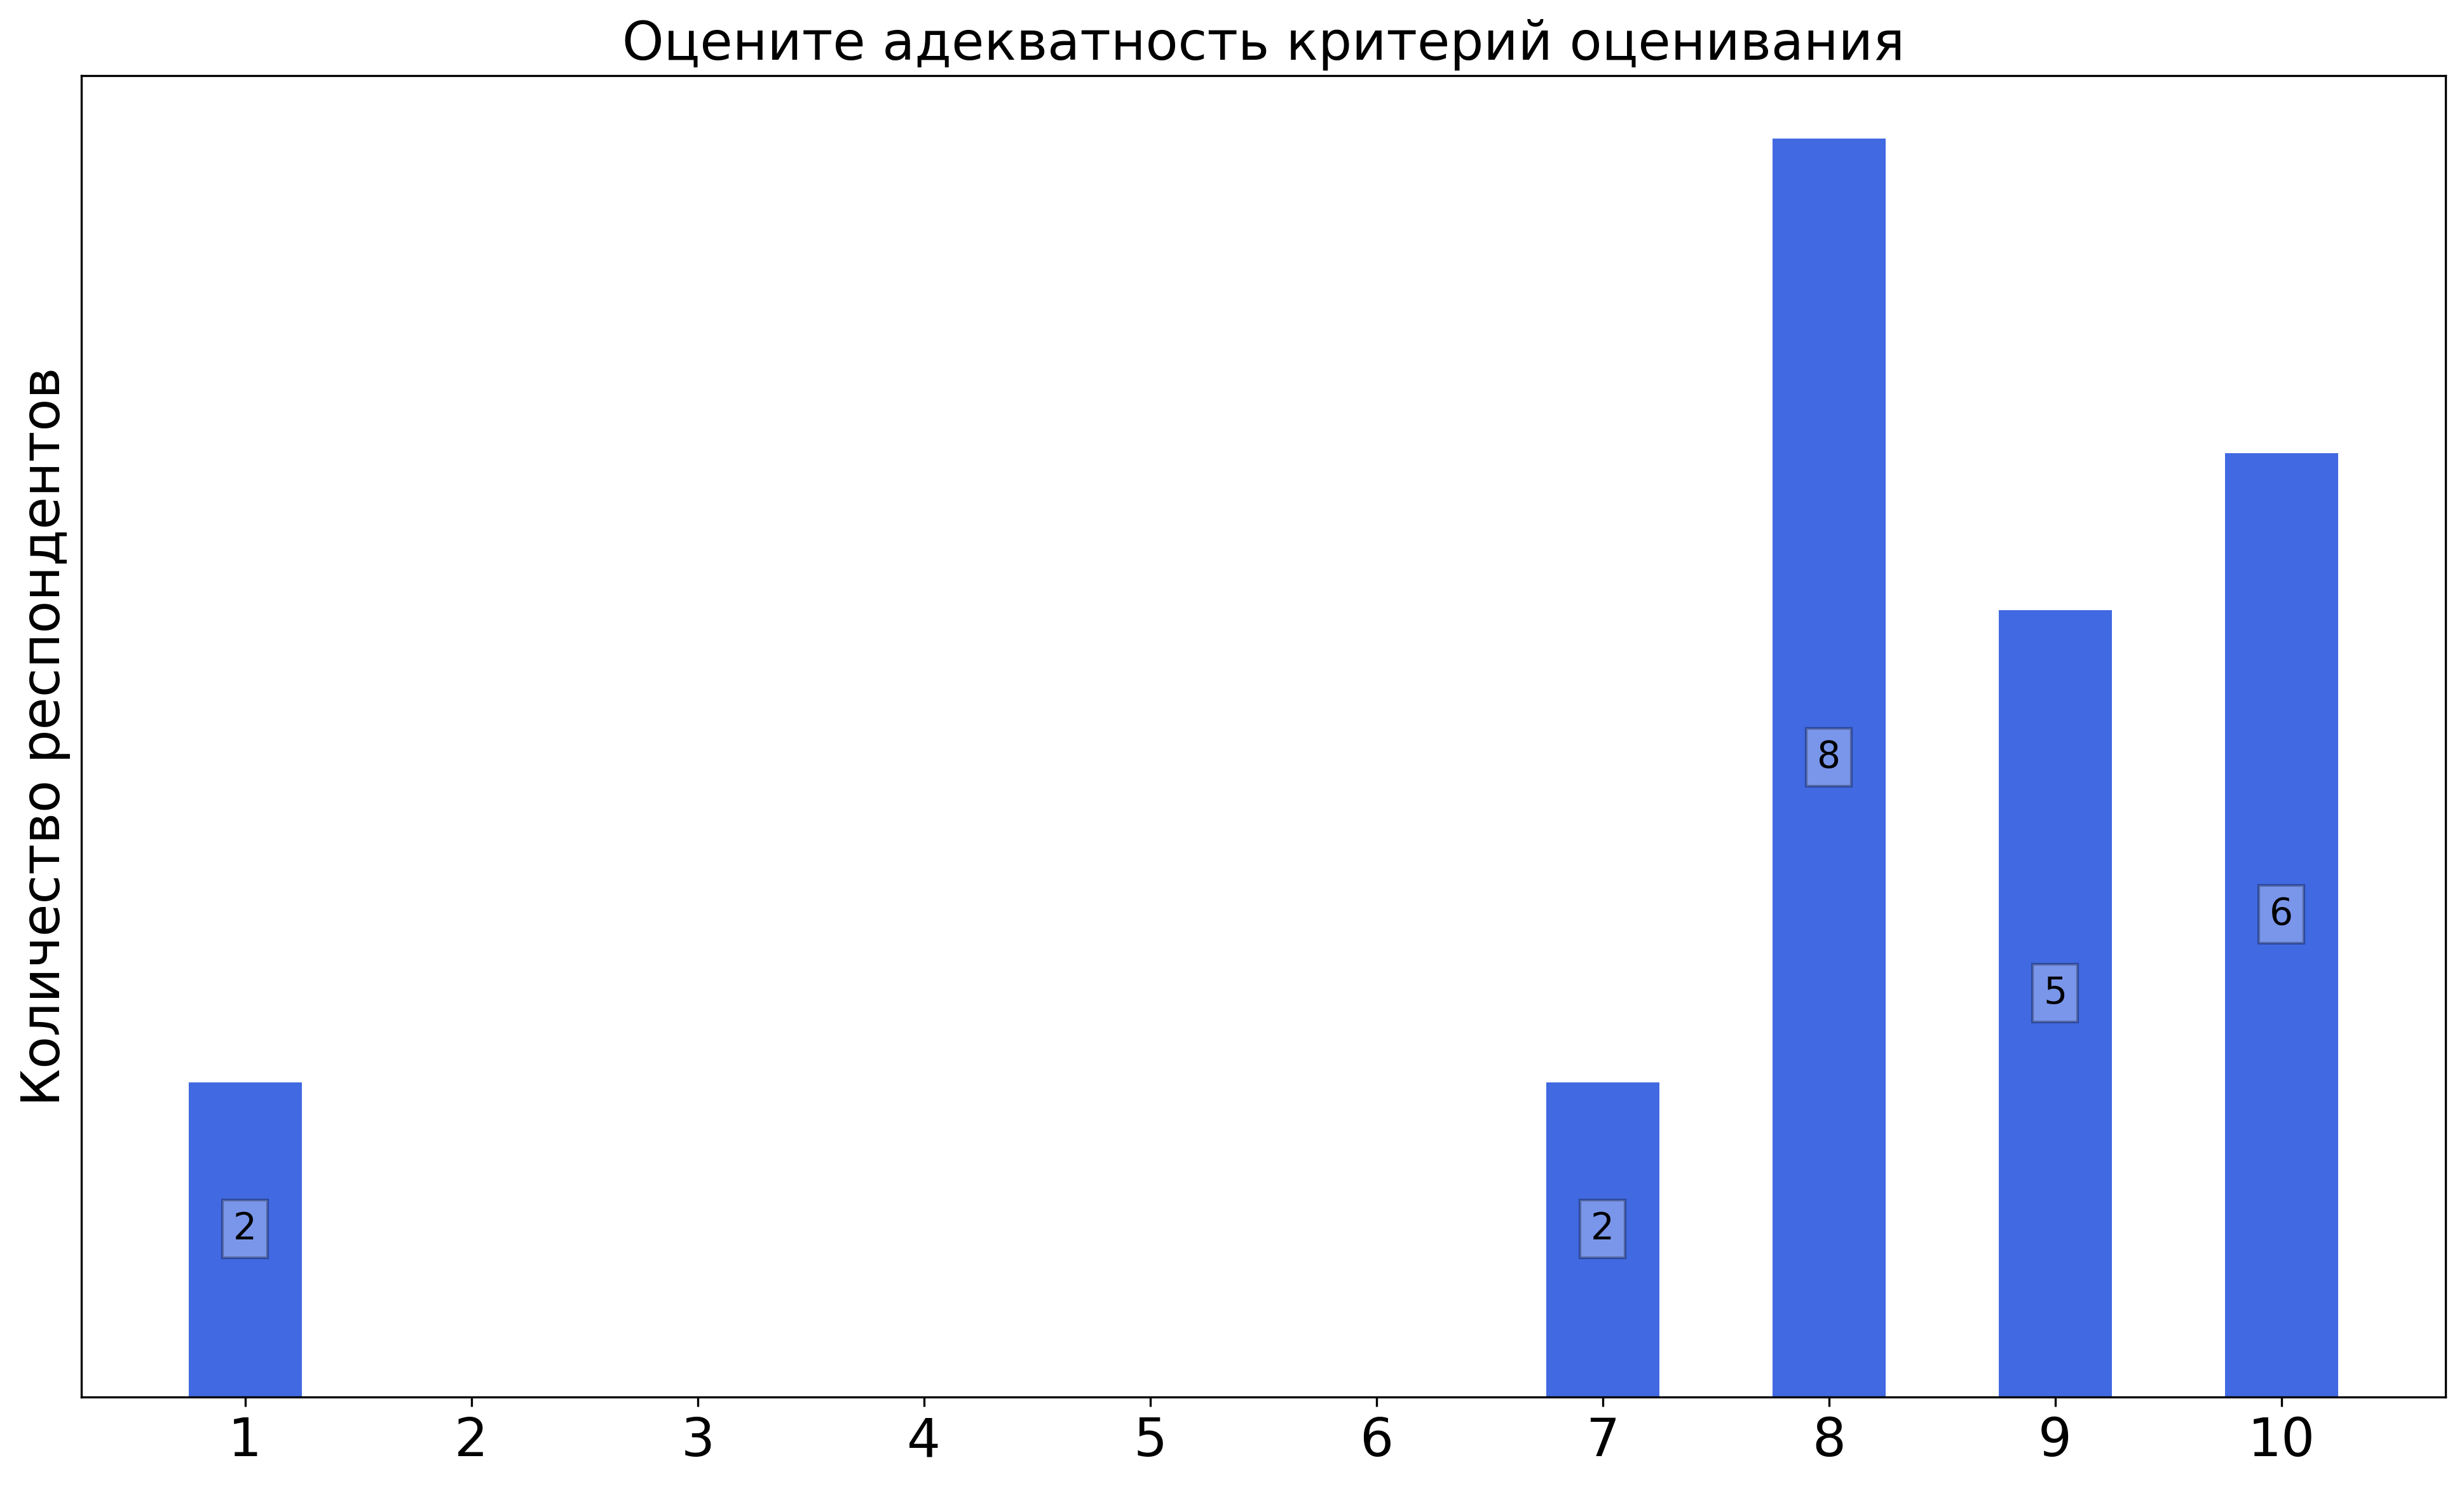
\includegraphics[width=\textwidth]{images/1 course/Аналитическая геометрия/seminarists-marks-Петрович А.А.-3.png}
            \end{subfigure}	
            \caption{Оценки респондентов о качестве преподавания семинаров}
        \end{figure}

        \textbf{Комментарии студентов о семинаристе\protect\footnote{сохранены оригинальные орфография и пунктуация}}
            \begin{commentbox} 
                Абсолютно не разбирается в материале. На семинарах просто считывает задачи с листка слово в слово. После ее семинаров в голове творится абсолютный хаос и непонимания методов решения задач. Не знает ответа ни на один вопрос. Либо говорит, что ответит на следующем семинаре, а сама копирует ответ из википедии абсолютно без понятия. БРС ставит хорошие. Контрольные можно переписывать, а задания досдавать. В этом ее преимущество. 
            \end{commentbox} 
        
            \begin{commentbox} 
                В общении есть что-то неприятное, будто Анна Александровна не очень хочет отвечать на вопрос. В остальном неспешное проведение семинара и полный разбор задач норм 
            \end{commentbox} 
        
            \begin{commentbox} 
                она вообще что-то понимает? 
            \end{commentbox} 
        
            \begin{commentbox} 
                Сложилось впечатление, что студенты знают больше, чем она 
            \end{commentbox} 
        
            \begin{commentbox} 
                Весь материал переписывается с листочка, но, как ни странно, этого чаще всего оказывается достаточно как для понимания теории в общих чертах, так и для самостоятельного решения задач 
            \end{commentbox} 
        
            \begin{commentbox} 
                Петрович на семинарах просто рассказывает чётко заготовленные примеры и задачи с листочка.
                Плюсы: всегда успевает рассказать всё, что нужно.
                Минусы: сама в предмете не шарит от слова совсем. 
            \end{commentbox} 
        
            \begin{commentbox} 
                весь материал переписывает с тетради, но материал качественный. Решения чаще всего понятны, но если иногда что-то спросить, качественного ответа может и не последовать. Но в целом отрицательных впечатлений нет 
            \end{commentbox} 
        
            \begin{commentbox} 
                К сожалению, на семинарах не удаётся порешать идейные задачи, пообсуждать красивые сюжеты 
            \end{commentbox}


    \subsubsection{Отзыв студентов о семинарах. Семинарист: Умнов Е.А.}
        \begin{figure}[H]
            \centering
            \begin{subfigure}[b]{0.45\textwidth}
                \centering
                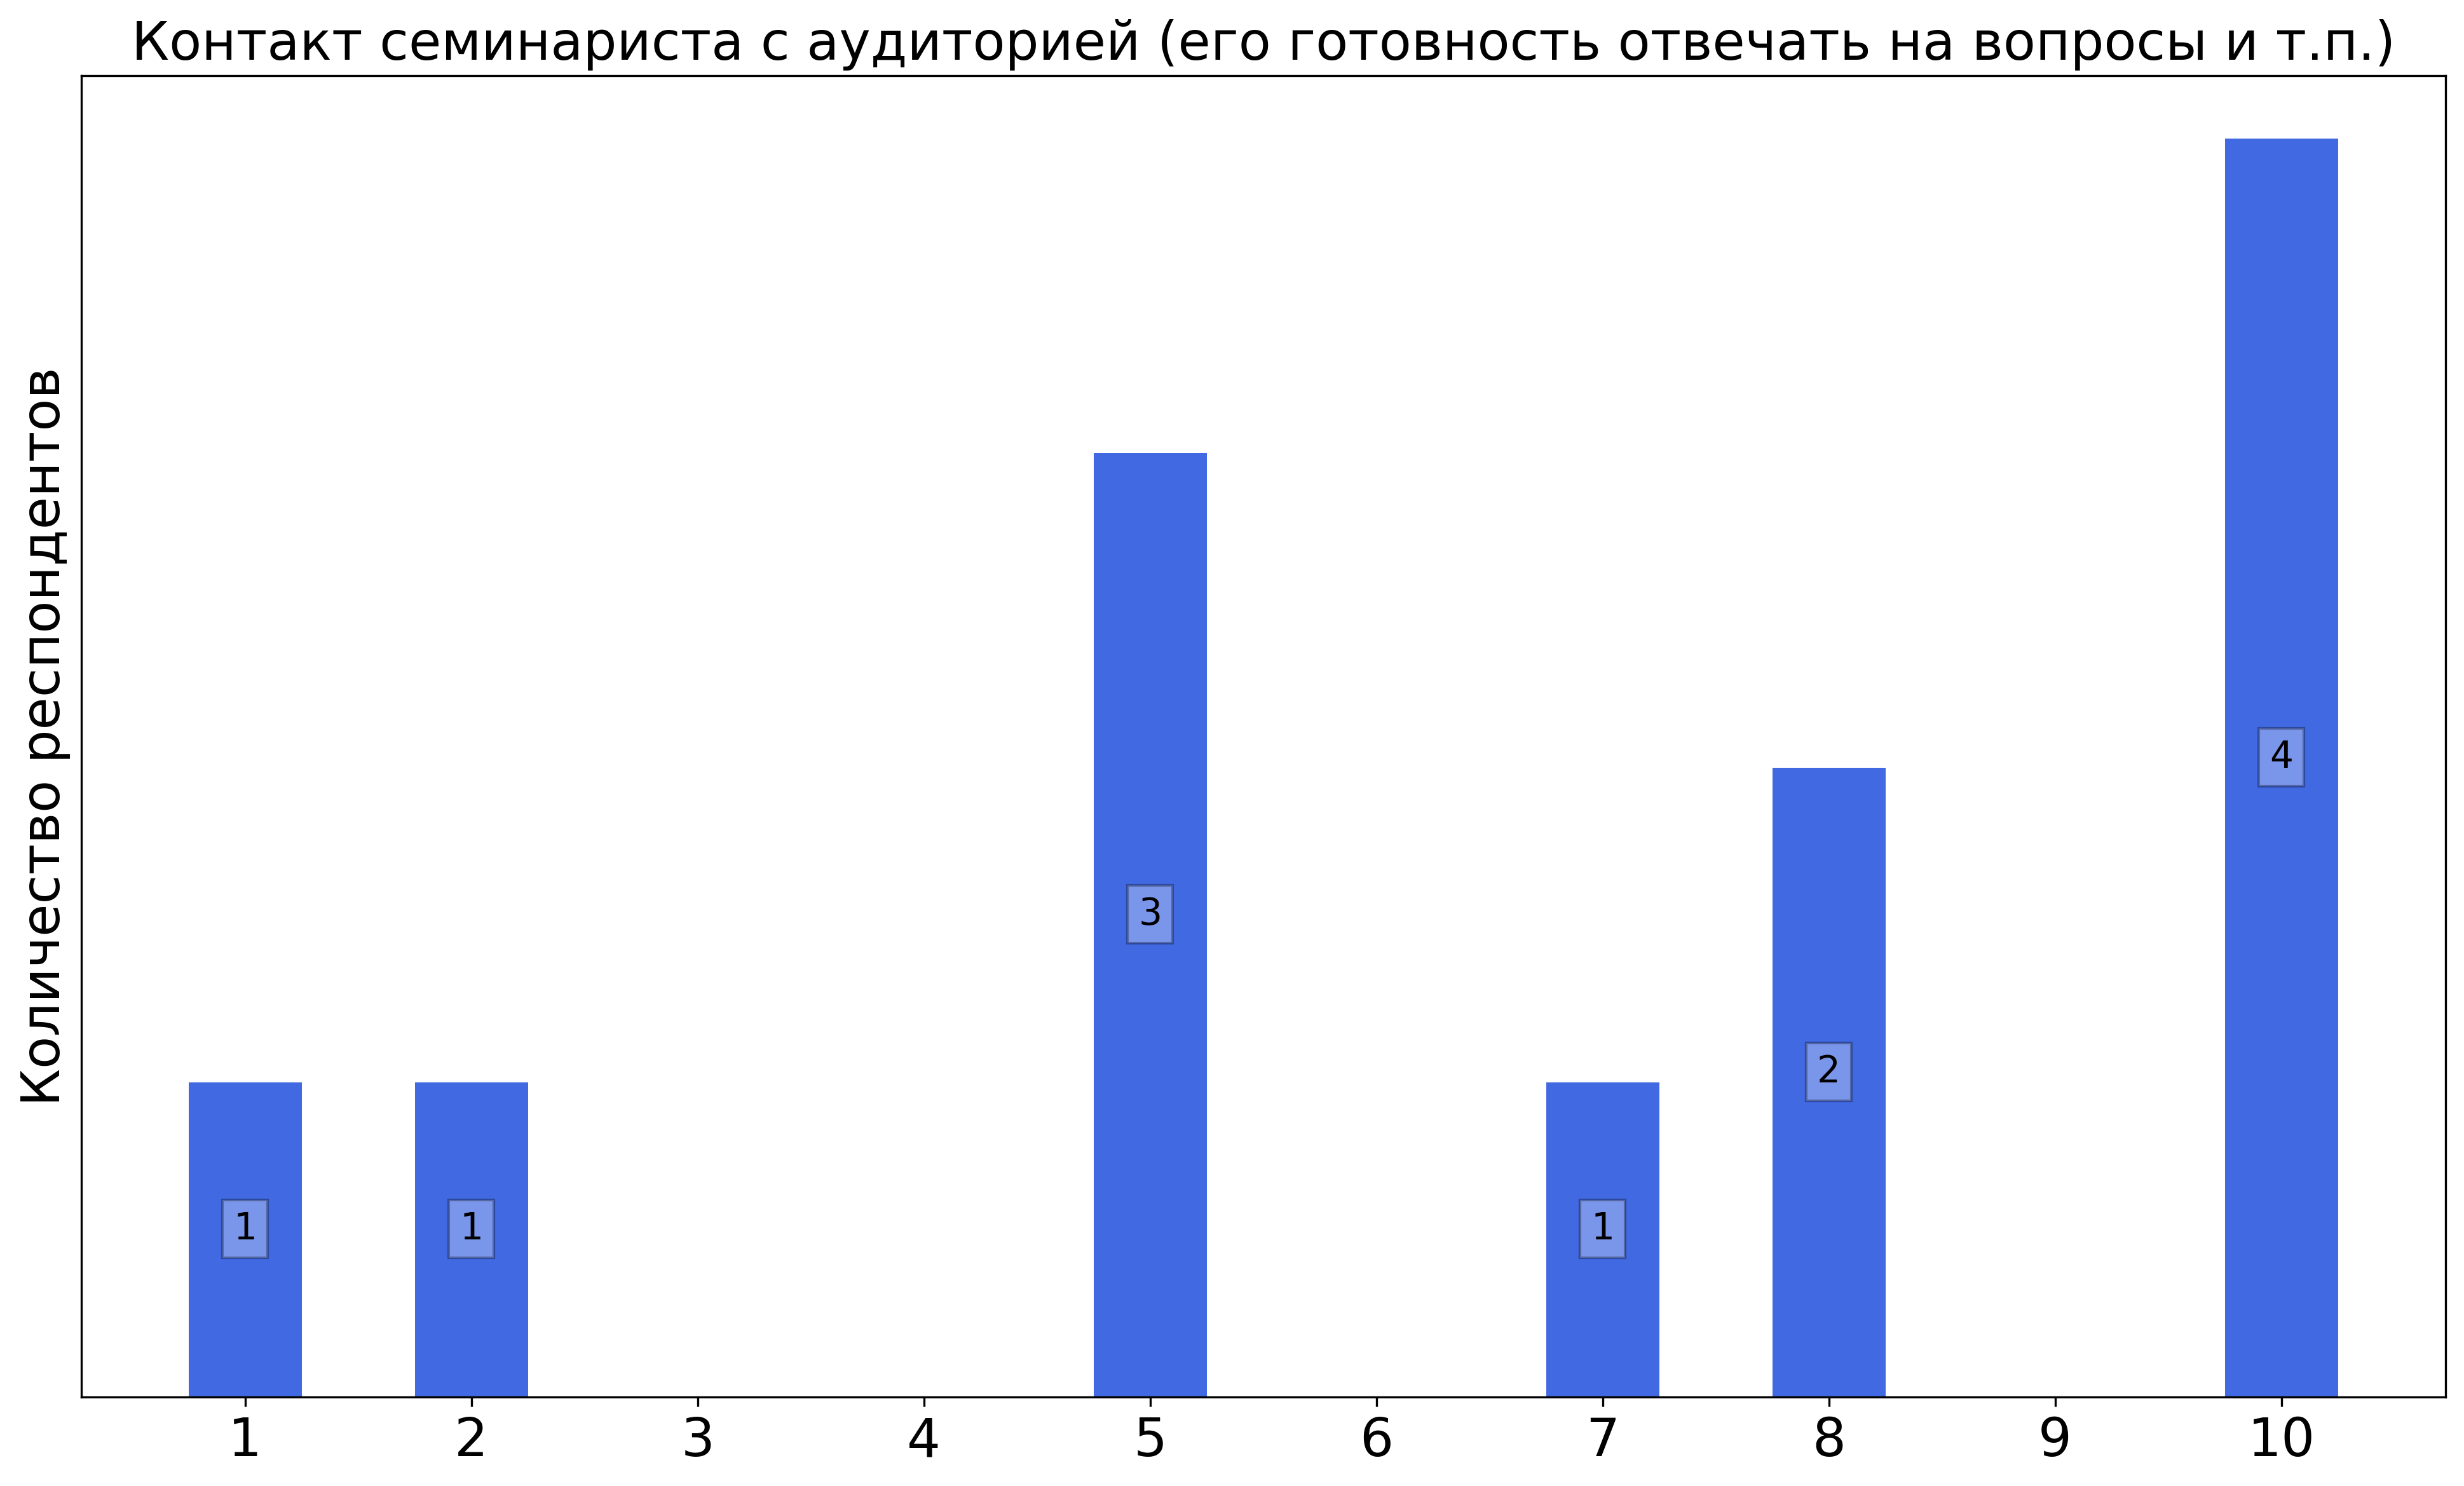
\includegraphics[width=\textwidth]{images/1 course/Аналитическая геометрия/seminarists-marks-Умнов Е.А.-0.png}
            \end{subfigure}
            \begin{subfigure}[b]{0.45\textwidth}
                \centering
                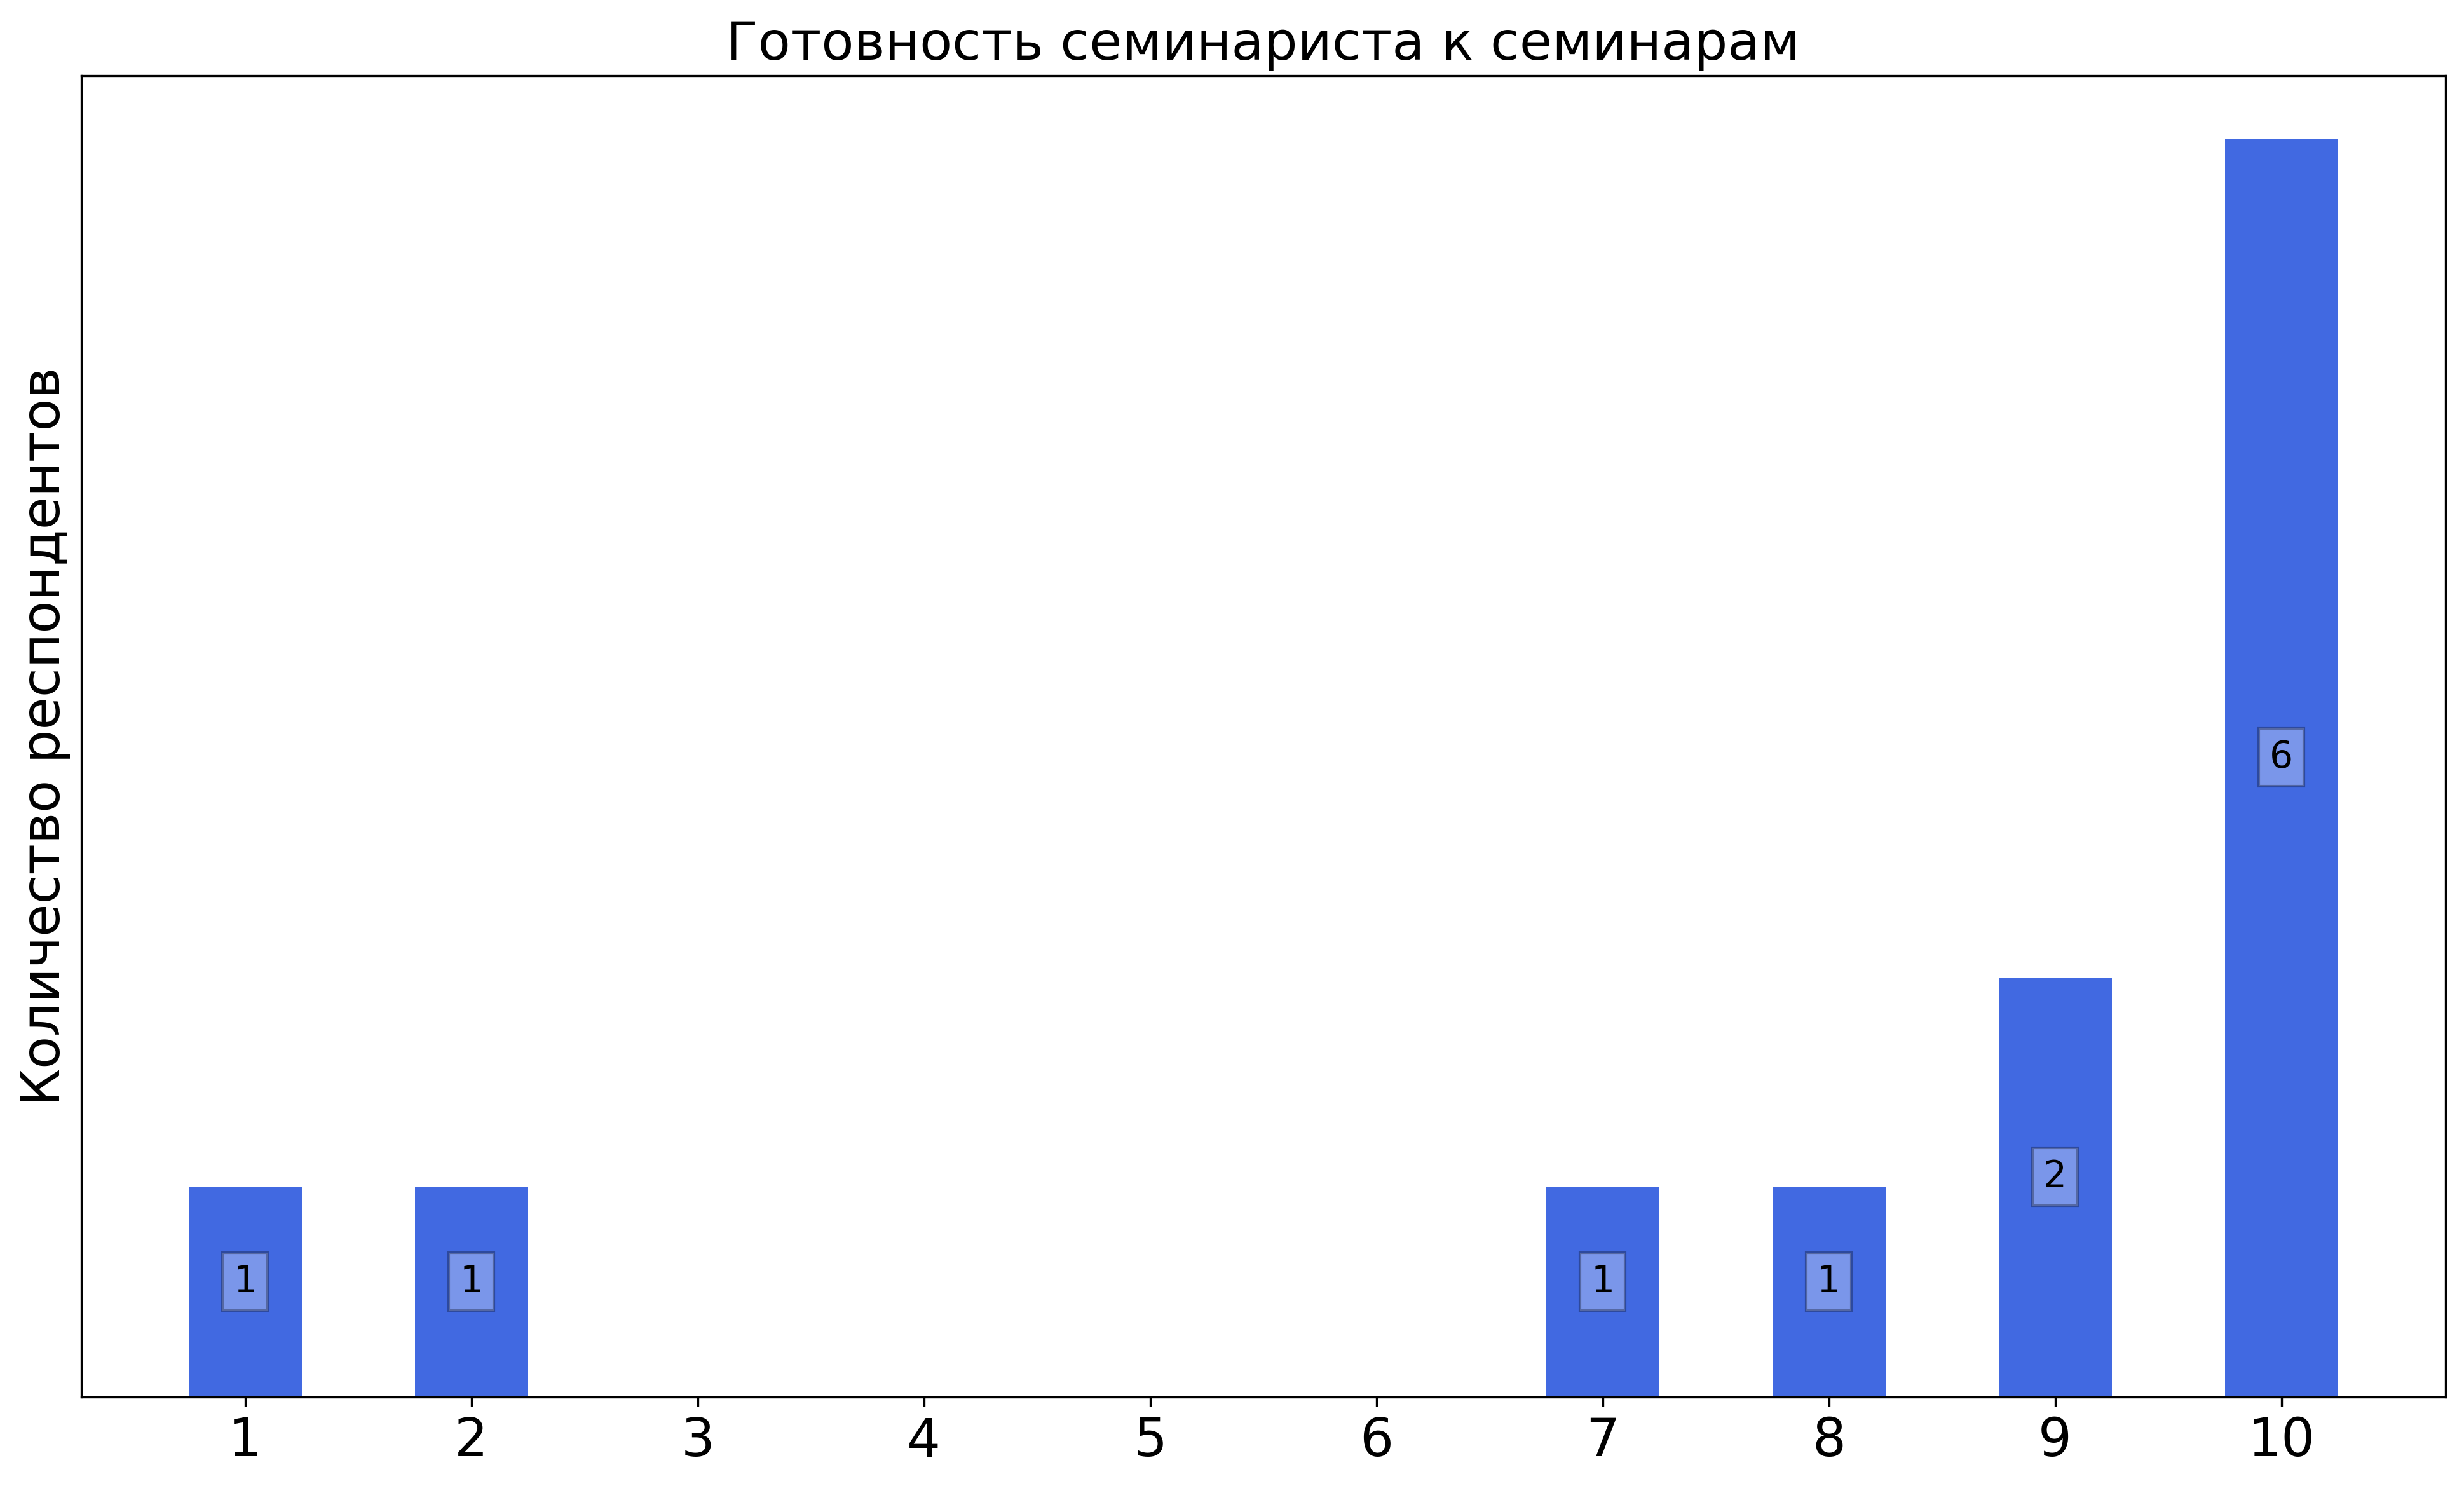
\includegraphics[width=\textwidth]{images/1 course/Аналитическая геометрия/seminarists-marks-Умнов Е.А.-1.png}
            \end{subfigure}
            \begin{subfigure}[b]{0.45\textwidth}
                \centering
                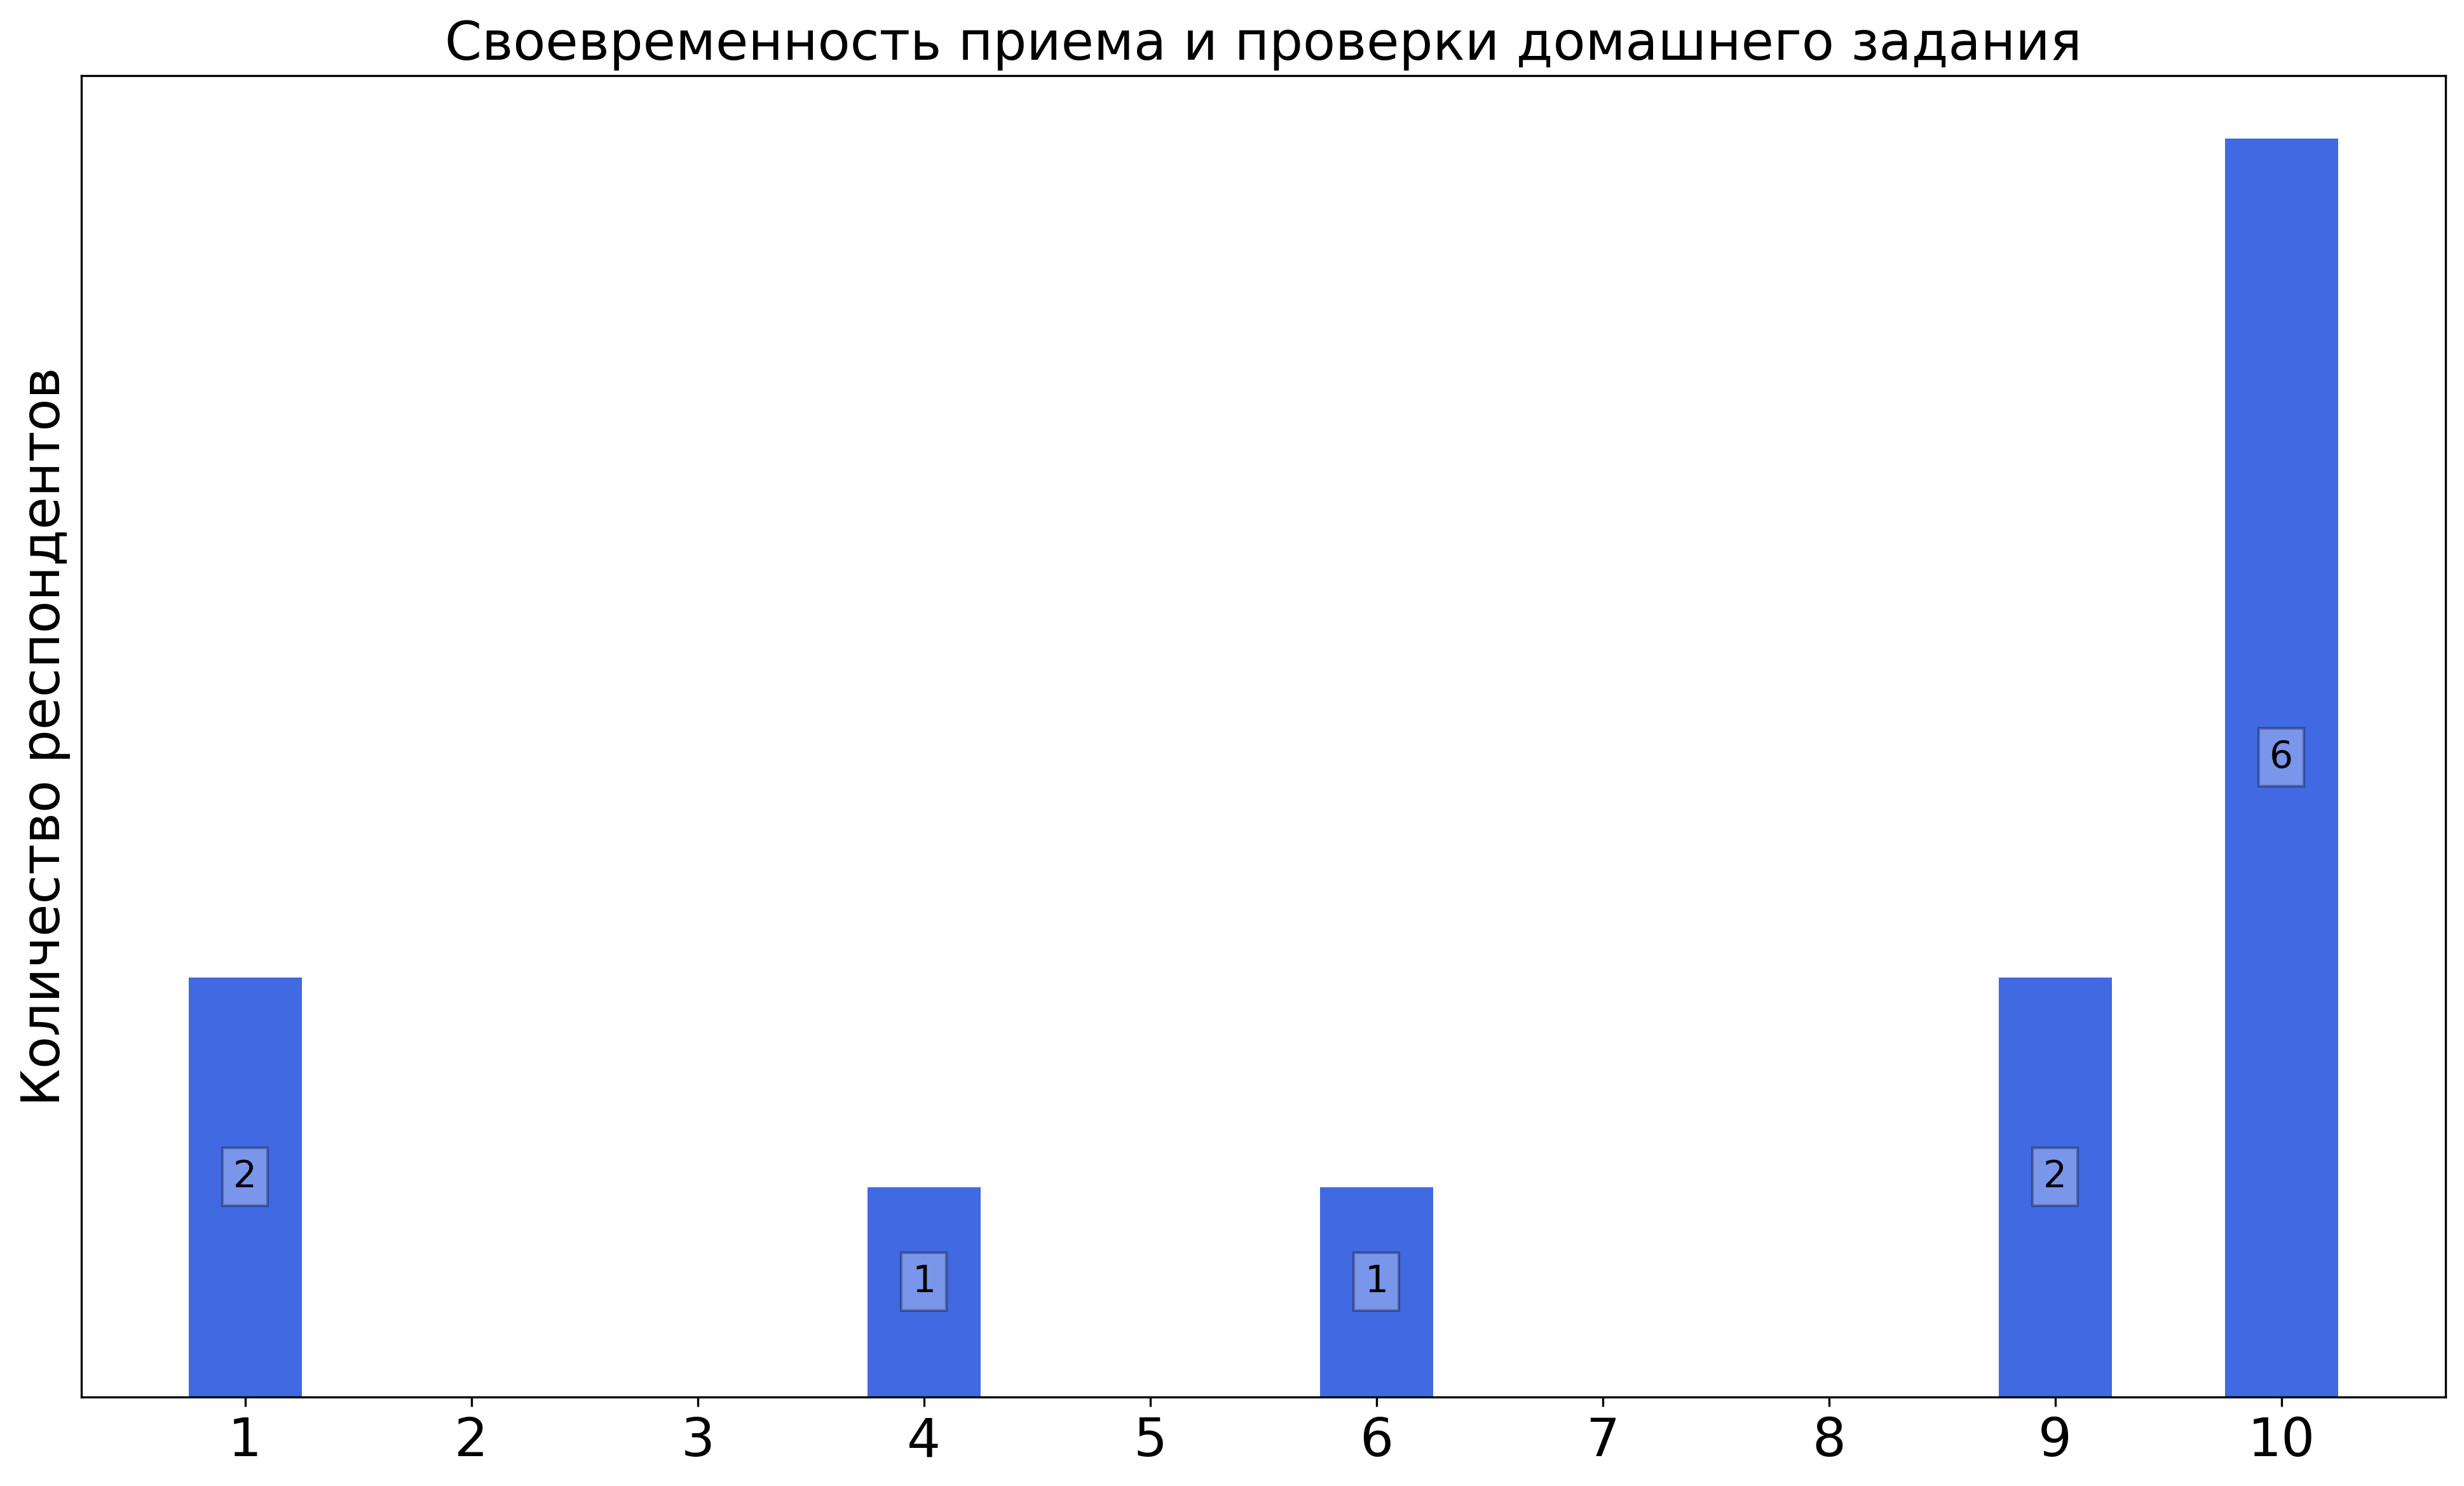
\includegraphics[width=\textwidth]{images/1 course/Аналитическая геометрия/seminarists-marks-Умнов Е.А.-2.png}
            \end{subfigure}
            \begin{subfigure}[b]{0.45\textwidth}
                \centering
                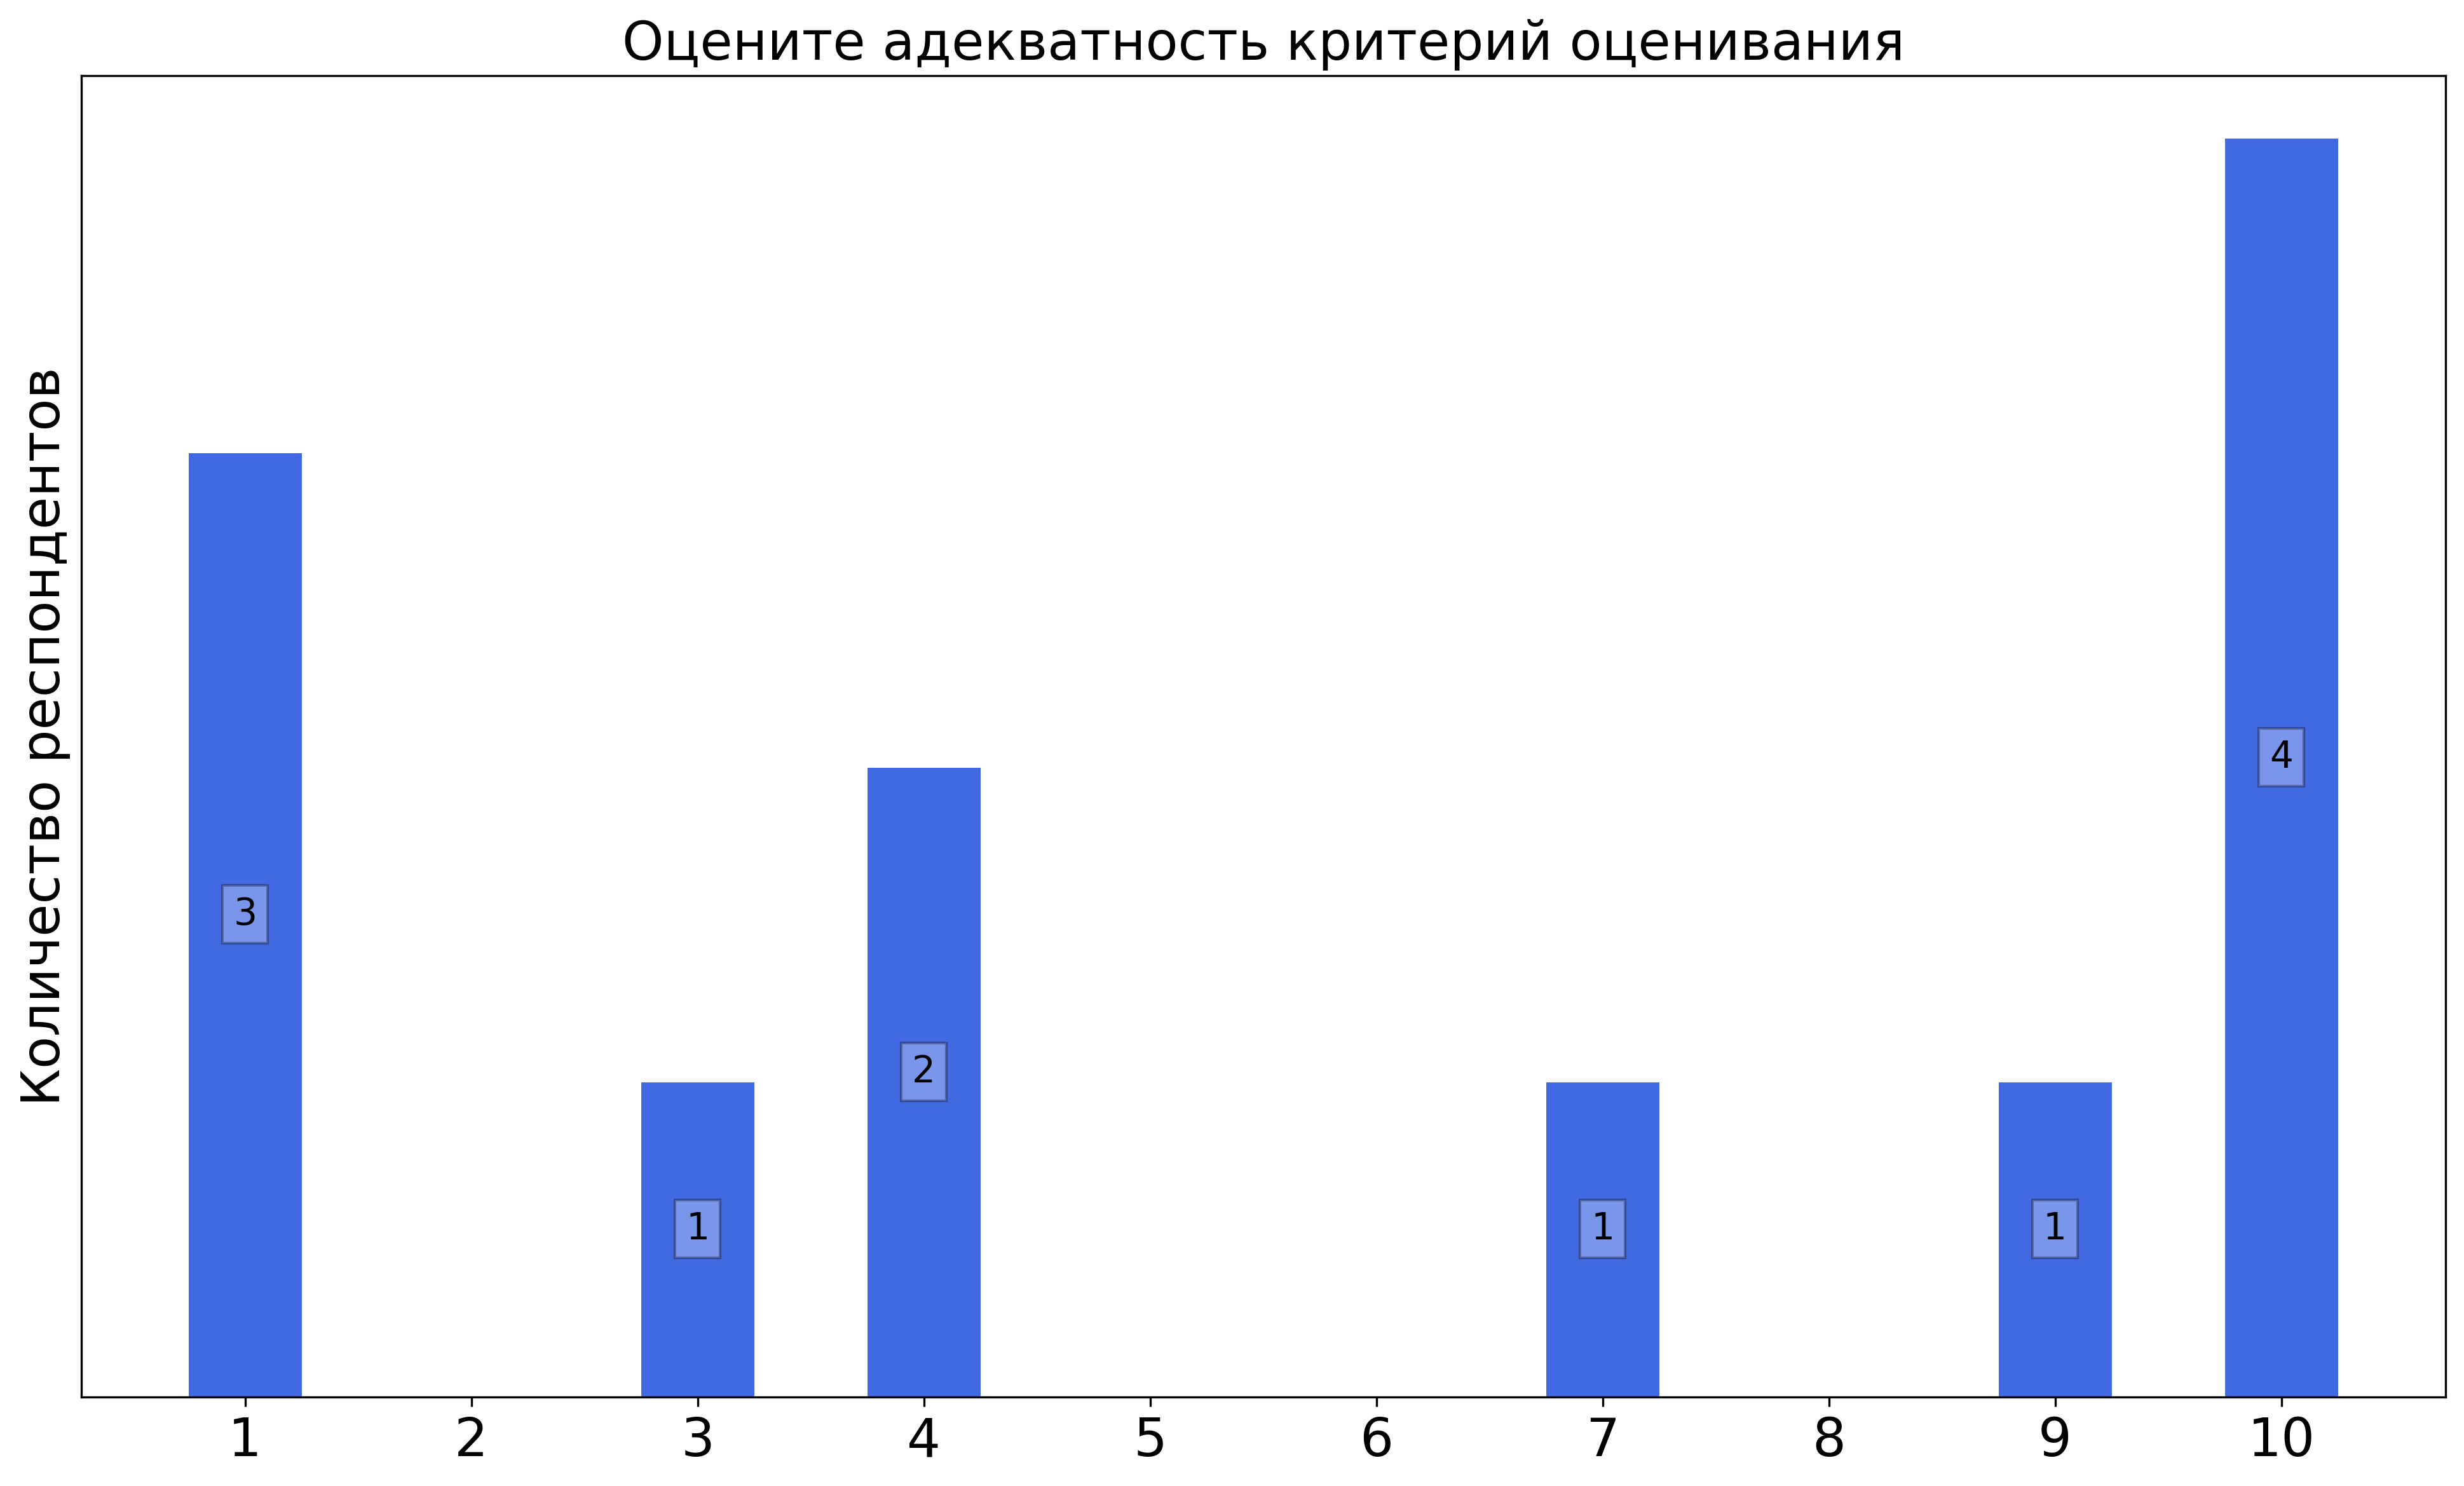
\includegraphics[width=\textwidth]{images/1 course/Аналитическая геометрия/seminarists-marks-Умнов Е.А.-3.png}
            \end{subfigure}	
            \caption{Оценки респондентов о качестве преподавания семинаров}
        \end{figure}

        \textbf{Комментарии студентов о семинаристе\protect\footnote{сохранены оригинальные орфография и пунктуация}}
            \begin{commentbox} 
                Почерк и скорость (реально быстро) желают лучшего 
            \end{commentbox} 
        
            \begin{commentbox} 
                Непонятно говорит и пишет. Зато очень спокойный и поможет разобраться в любом вопросе, терпеливо отвечая на все вопросы. 
            \end{commentbox} 
        
            \begin{commentbox} 
                Слушать очень тяжело и тяжело понимать что он пишет  
            \end{commentbox} 
        
            \begin{commentbox} 
                Как семинарист умнов не так уж и плох, но ужасная лекция и строгая система оценивания, душно 
            \end{commentbox}
        
        
    \subsubsection{Отзыв студентов о семинарах. Семинарист: Чубаров И.А.}
        \begin{figure}[H]
            \centering
            \begin{subfigure}[b]{0.45\textwidth}
                \centering
                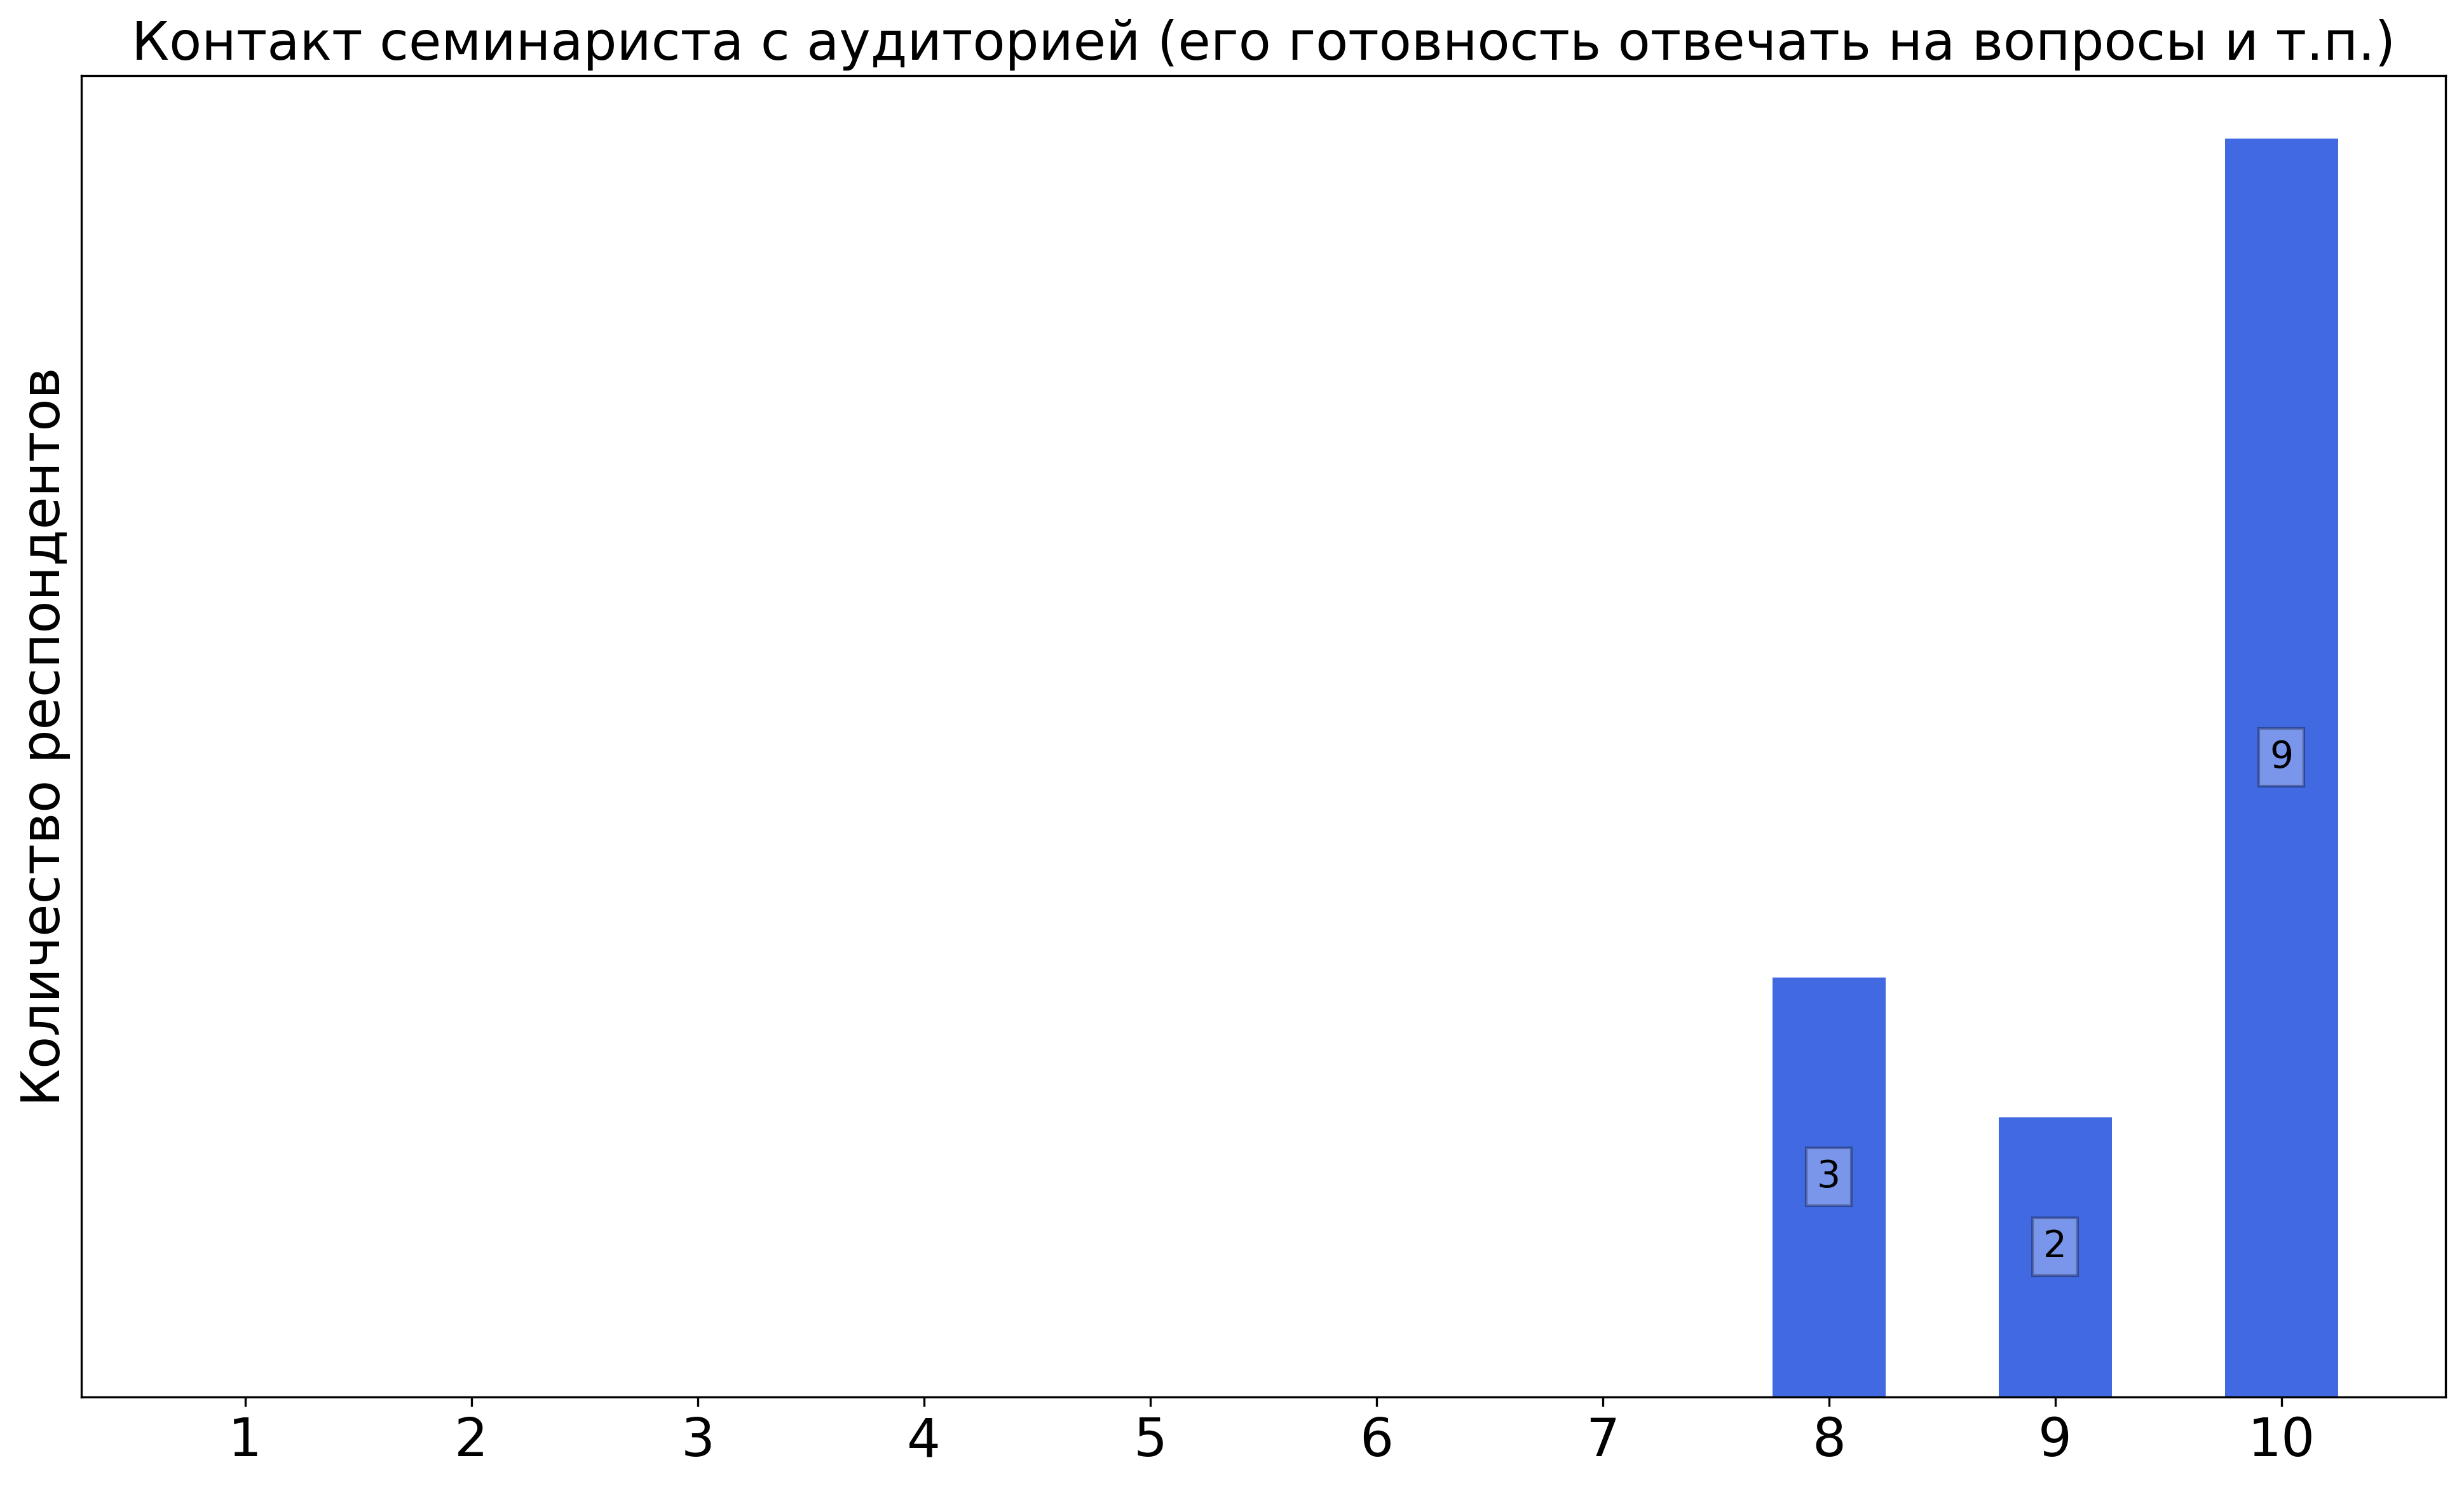
\includegraphics[width=\textwidth]{images/1 course/Аналитическая геометрия/seminarists-marks-Чубаров И.А.-0.png}
            \end{subfigure}
            \begin{subfigure}[b]{0.45\textwidth}
                \centering
                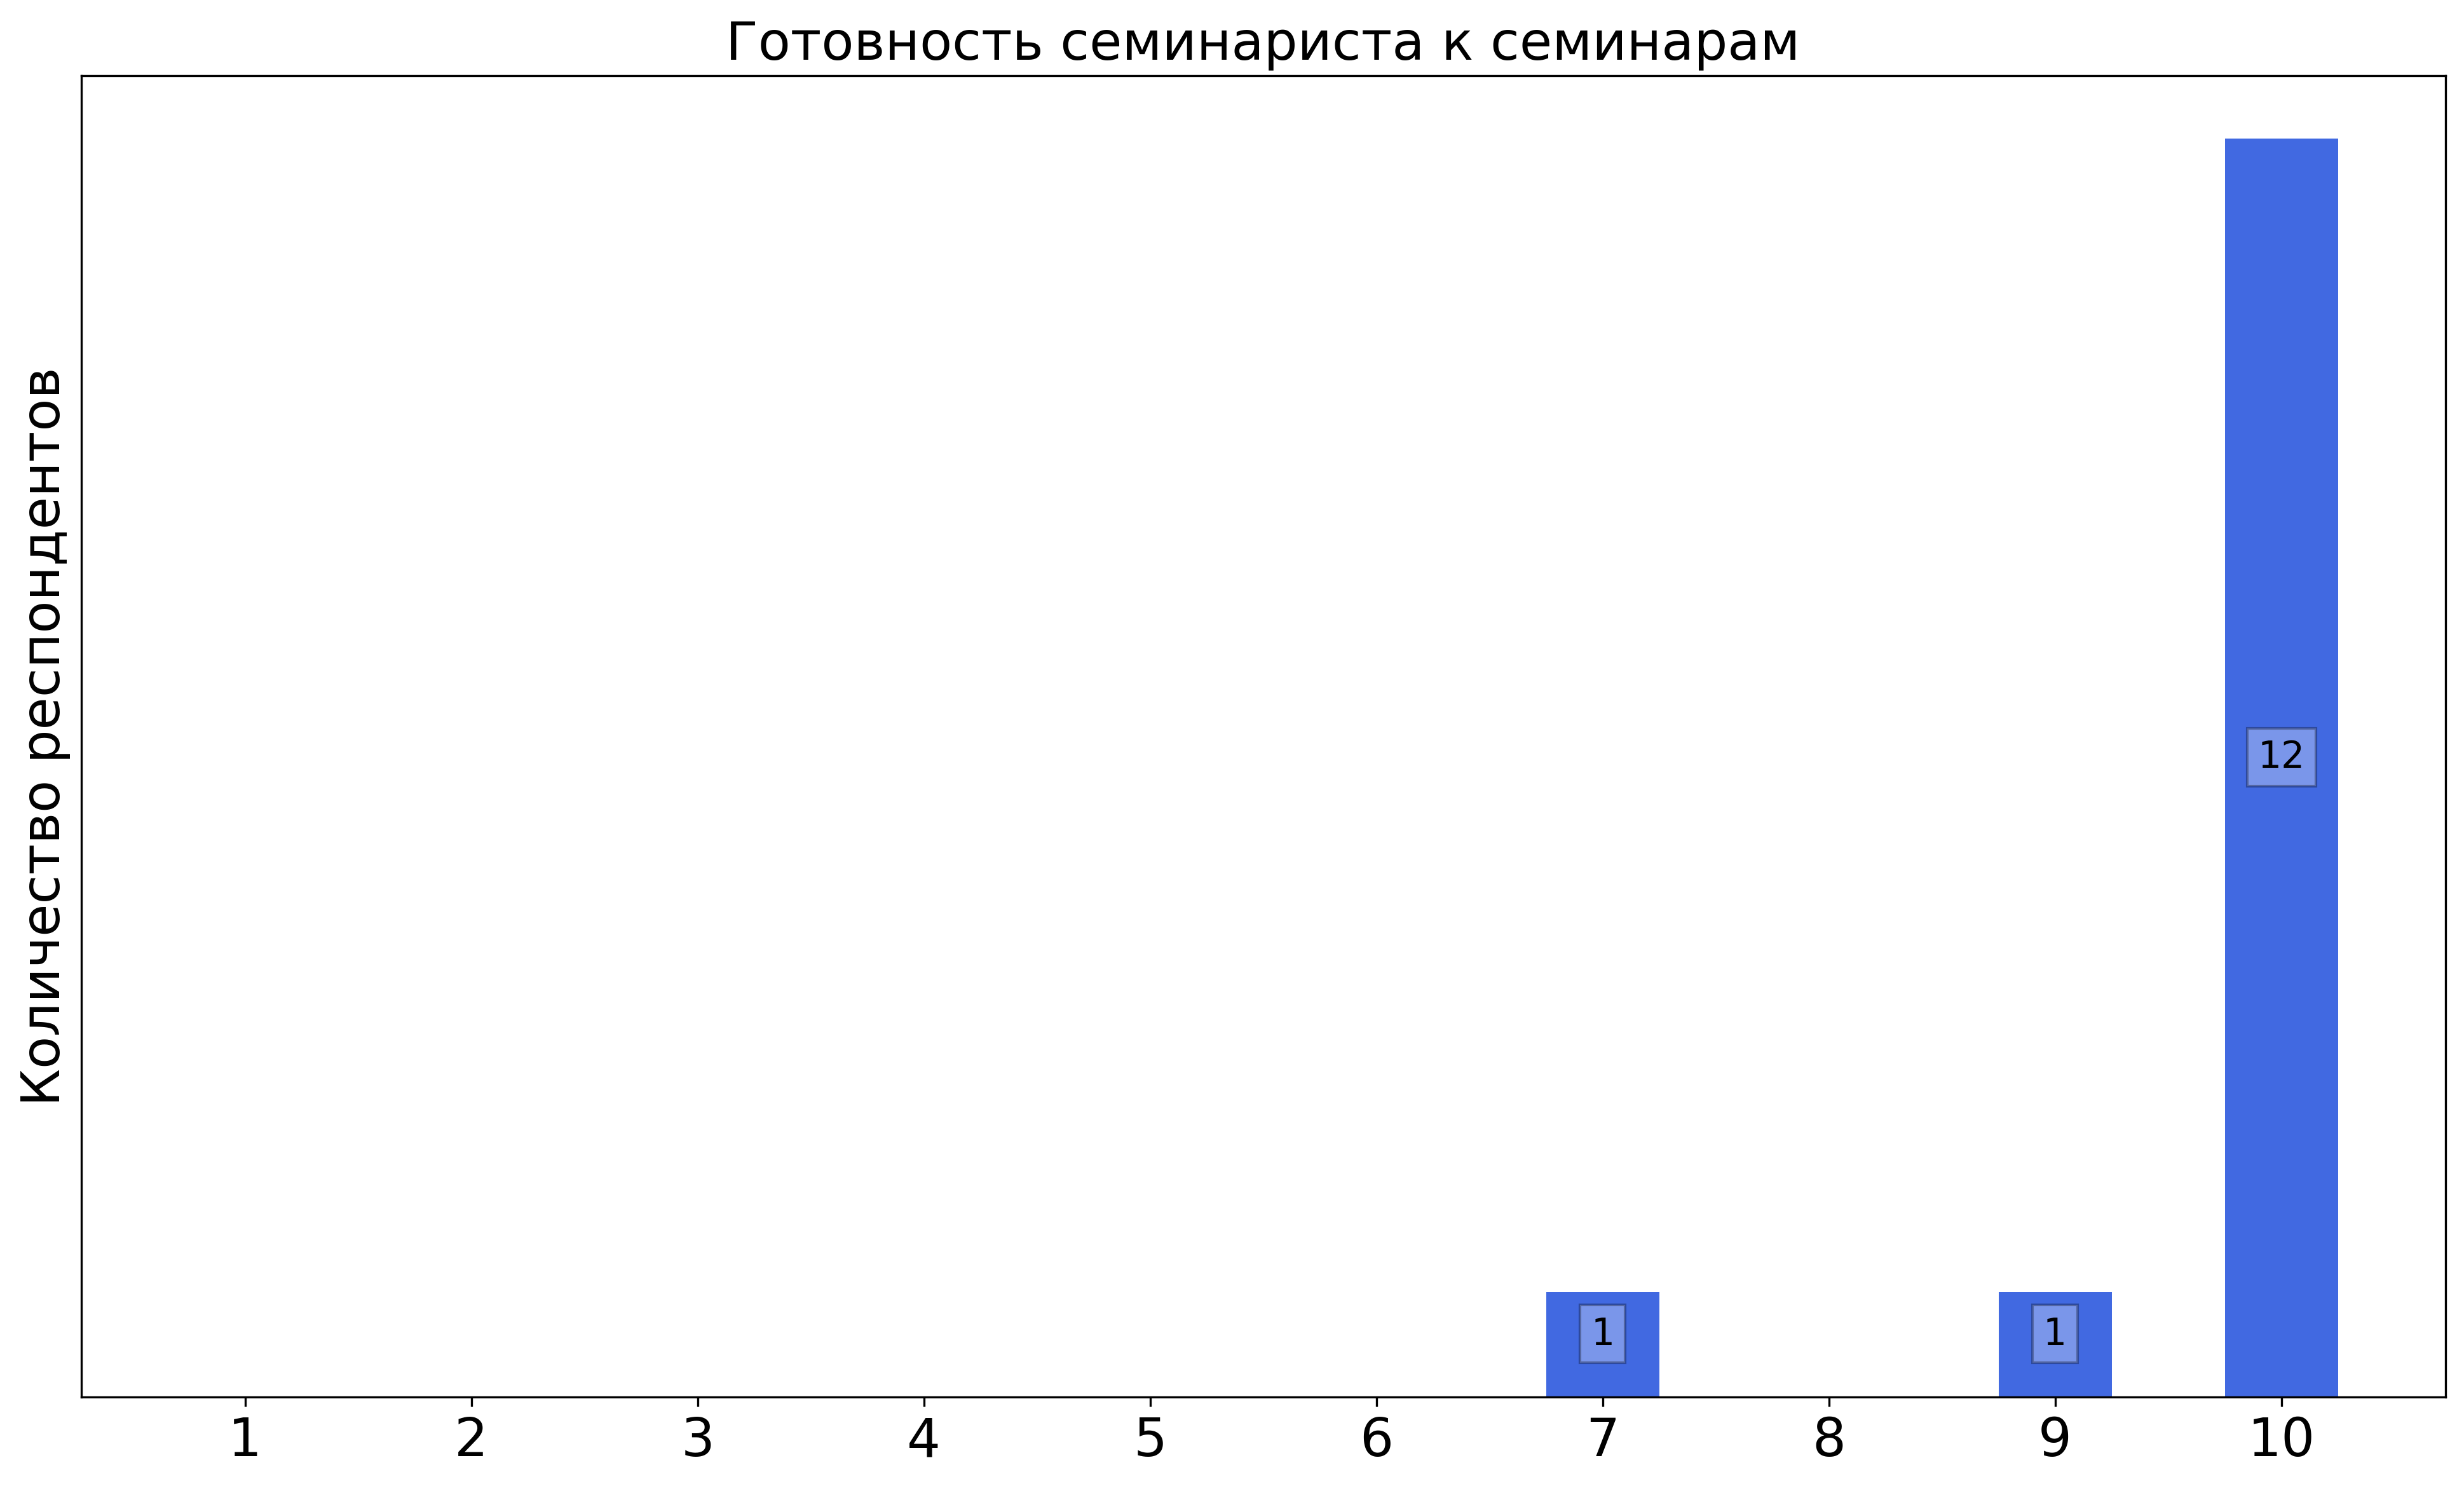
\includegraphics[width=\textwidth]{images/1 course/Аналитическая геометрия/seminarists-marks-Чубаров И.А.-1.png}
            \end{subfigure}
            \begin{subfigure}[b]{0.45\textwidth}
                \centering
                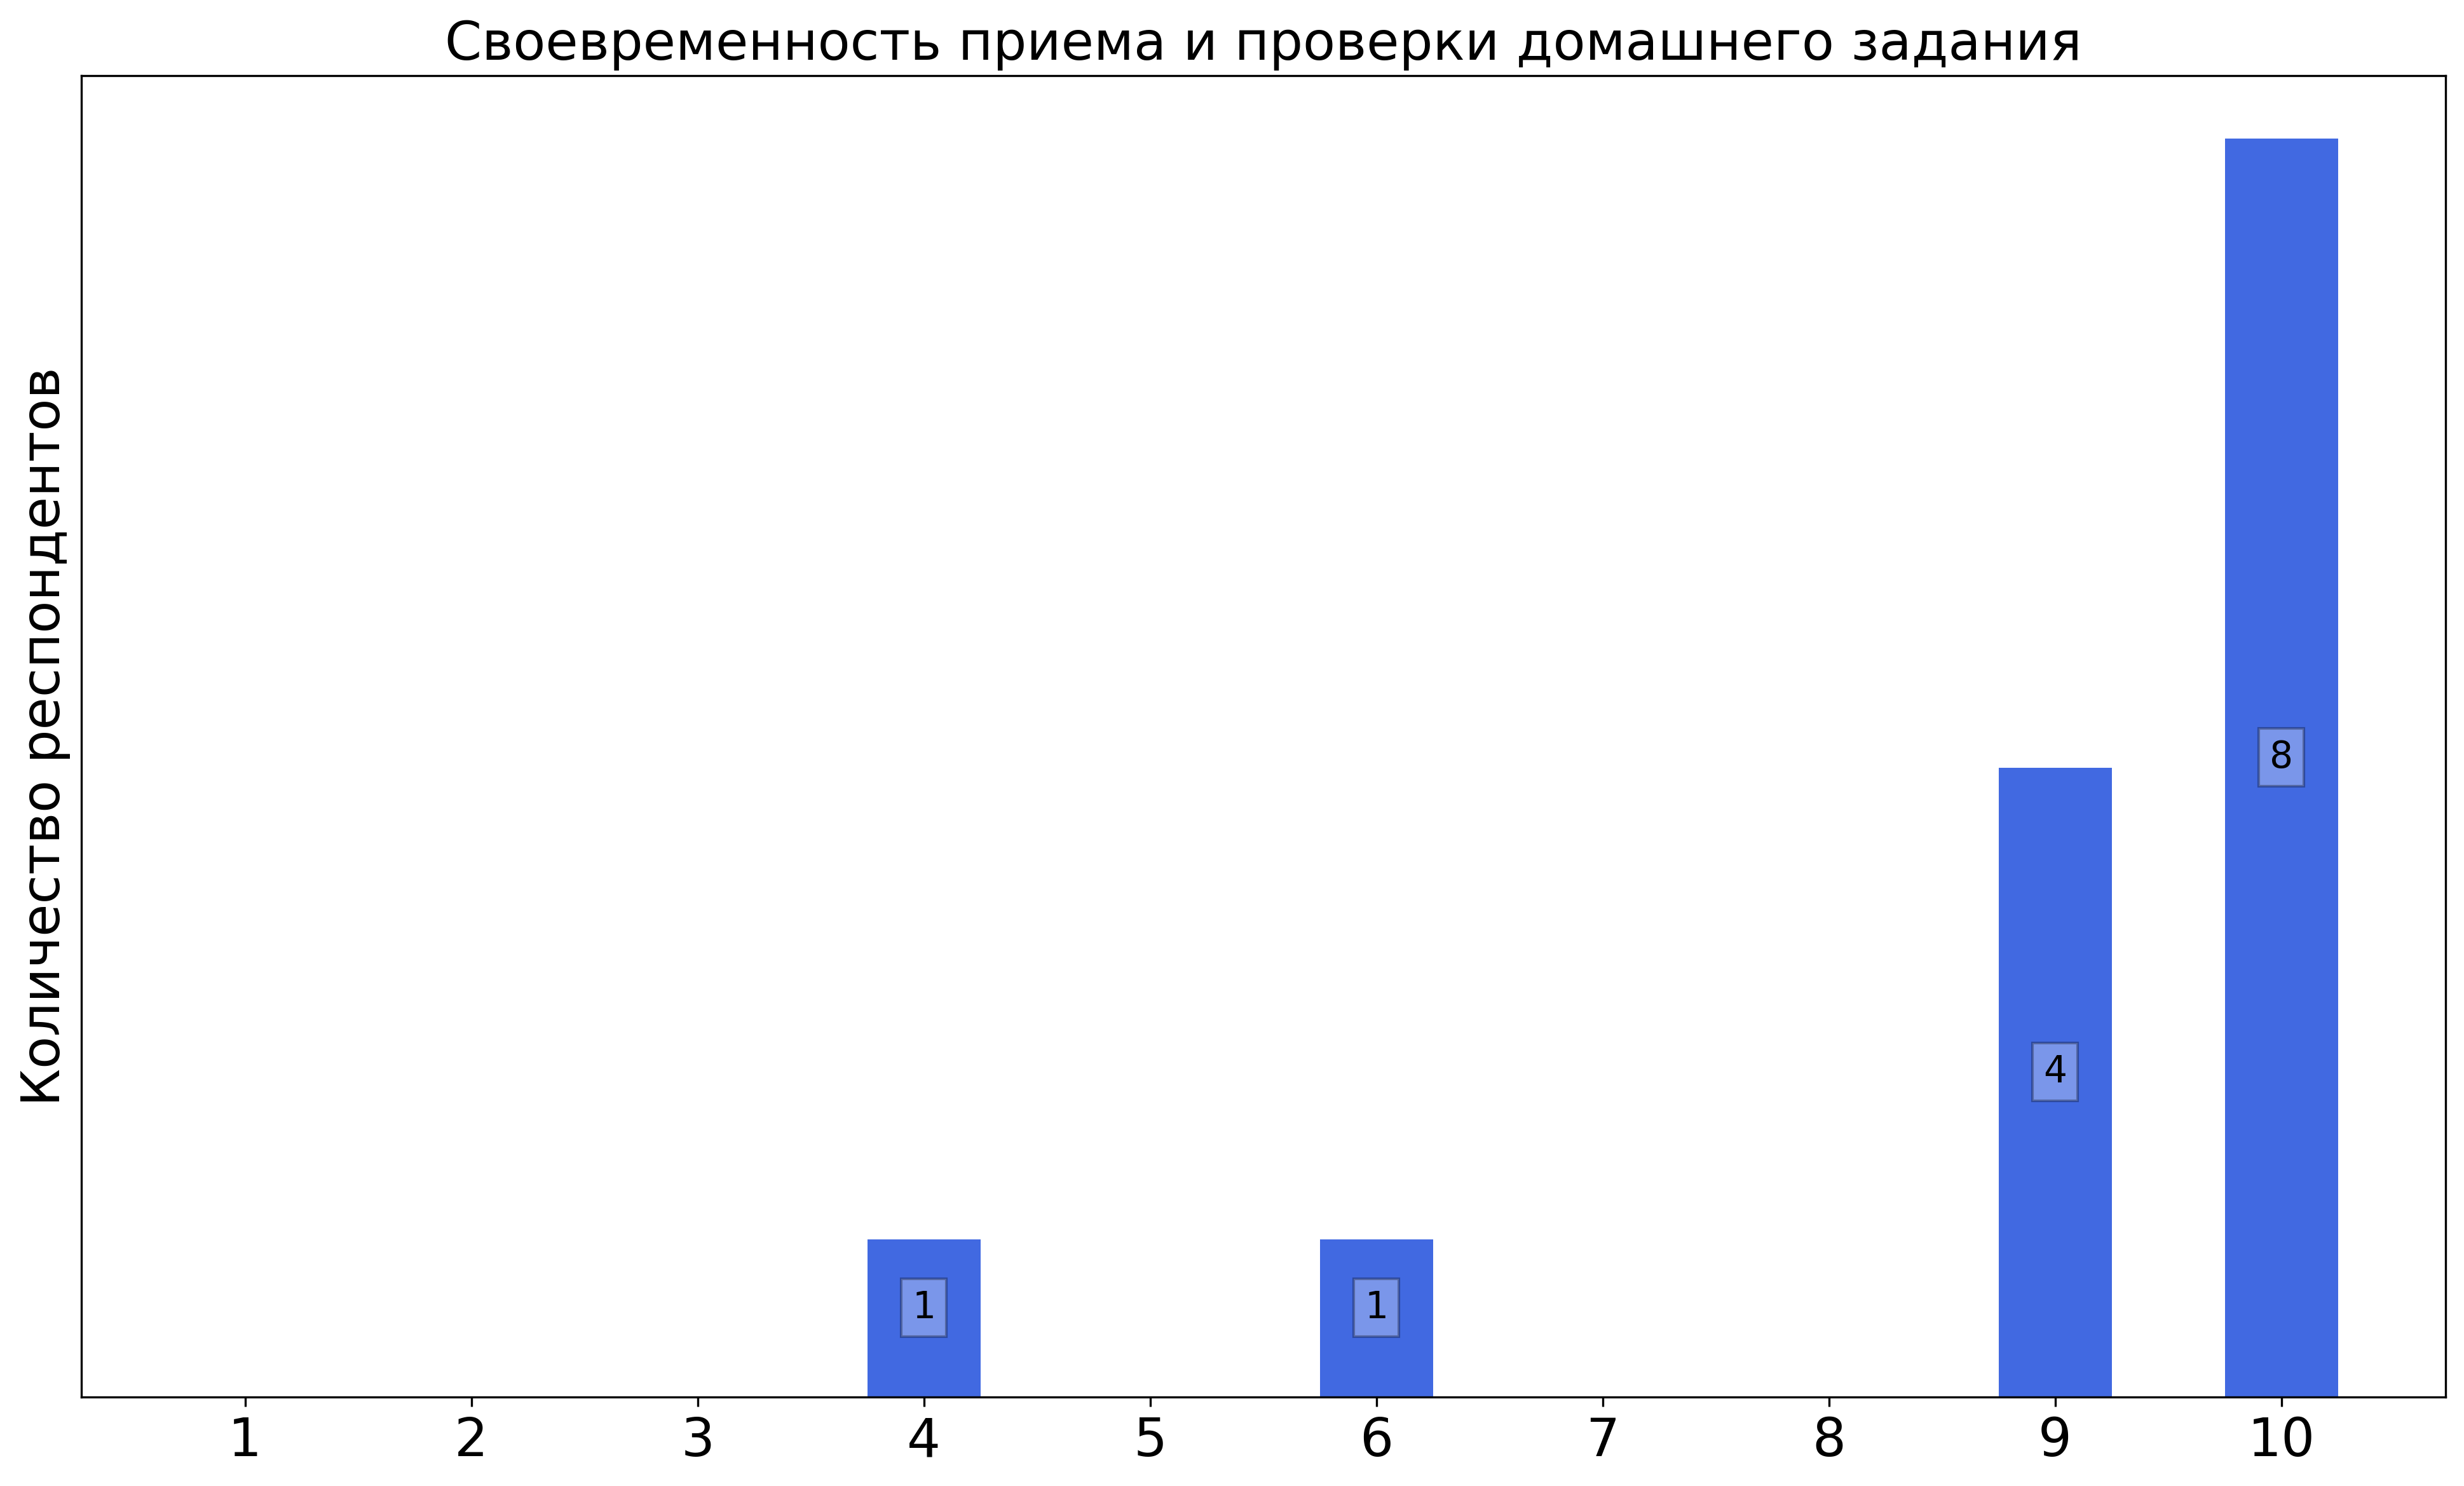
\includegraphics[width=\textwidth]{images/1 course/Аналитическая геометрия/seminarists-marks-Чубаров И.А.-2.png}
            \end{subfigure}
            \begin{subfigure}[b]{0.45\textwidth}
                \centering
                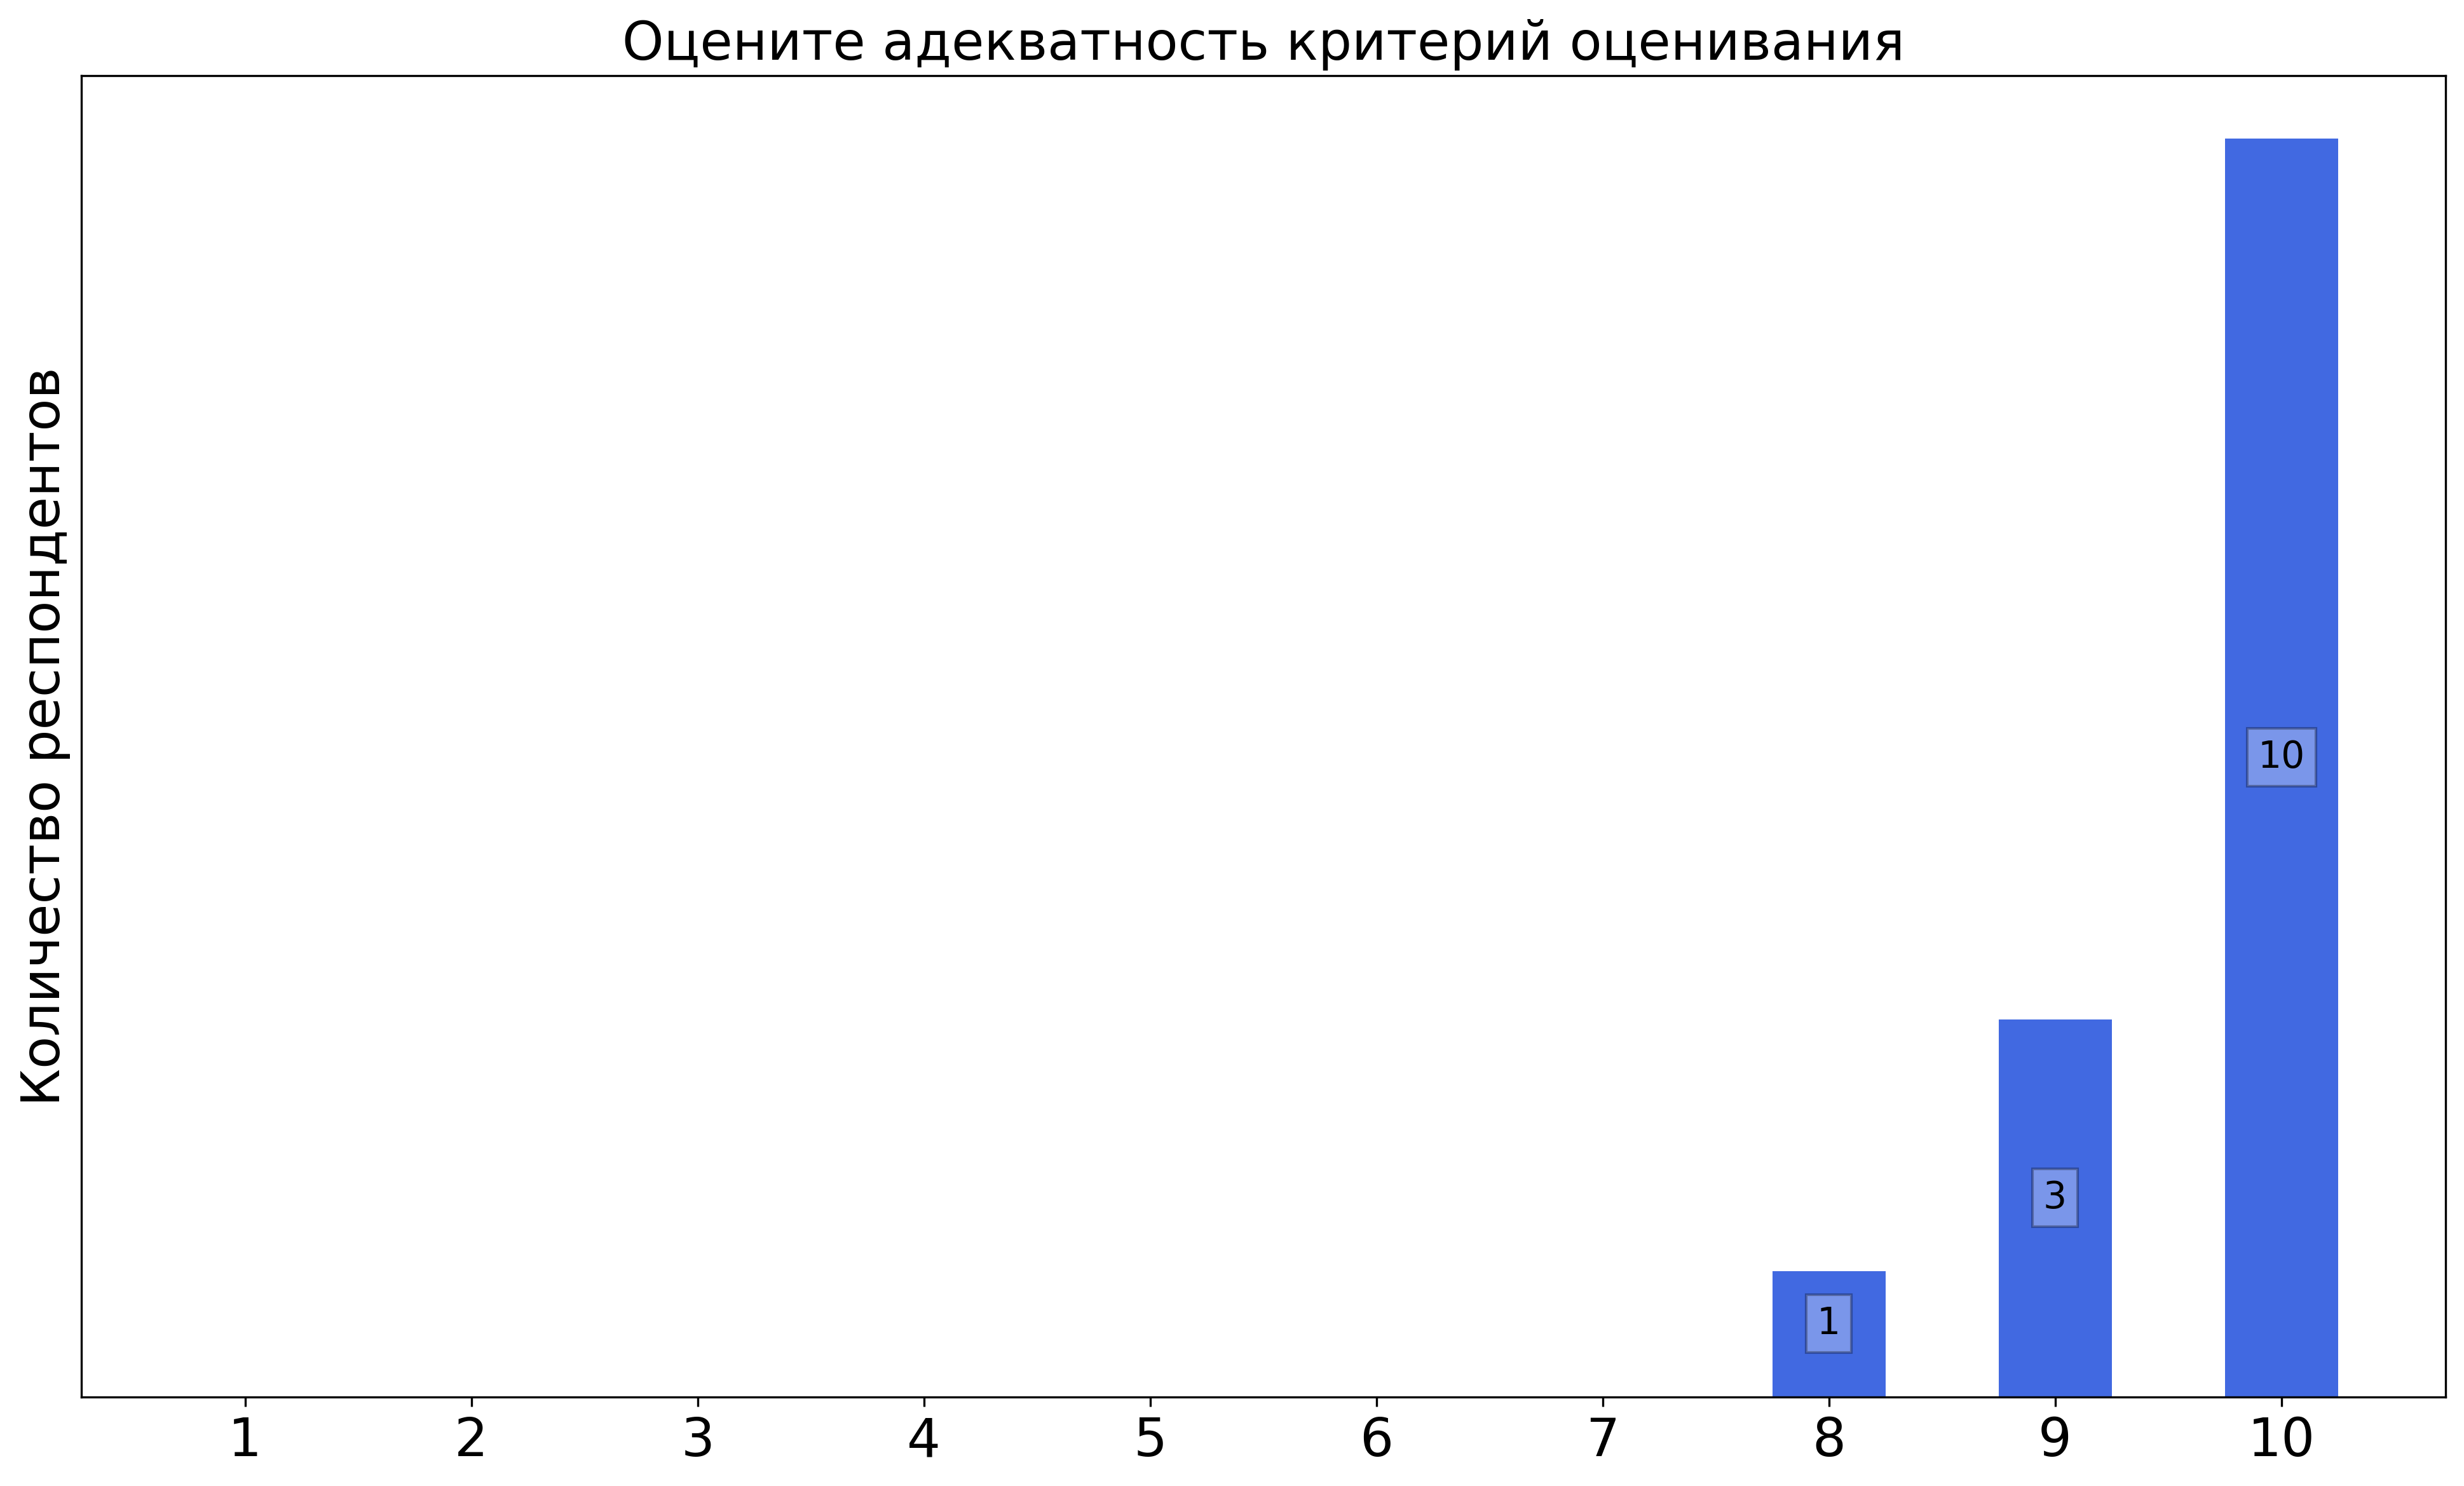
\includegraphics[width=\textwidth]{images/1 course/Аналитическая геометрия/seminarists-marks-Чубаров И.А.-3.png}
            \end{subfigure}	
            \caption{Оценки респондентов о качестве преподавания семинаров}
        \end{figure}

        \textbf{Комментарии студентов о семинаристе\protect\footnote{сохранены оригинальные орфография и пунктуация}}
            \begin{commentbox} 
                Это прекрасно  
            \end{commentbox} 
        
            \begin{commentbox} 
                Очень добрый, задачи интересно с ним решать 
            \end{commentbox} 
        
            \begin{commentbox} 
                Все понравилось 
            \end{commentbox} 
        
            \begin{commentbox} 
                Отличный семинарист. Не знаю, что сказать 
            \end{commentbox} 
        
            \begin{commentbox} 
                Не много успевал решать на семинарах, иногда приходилось разбираться самому 
            \end{commentbox} 
        

    \subsubsection{Прочие комментарии и предложения по улучшению курса}
        \begin{commentbox}
            По-моему единственный нормальный курс, где и хороший семинарист и лектор понятно всё читает
        \end{commentbox}

        \begin{commentbox}
            В целом всё отлично 
        \end{commentbox}

        \begin{commentbox}
            Семинары шли быстрее лекций, так что процесс обучения получился наоборот, от практики к теории. Вероятно, это стоит пофиксить
        \end{commentbox}

        \begin{commentbox}
            Чтоб экзамен нормально принимали. Понятно, что эта проблема вековая. Но именно на ангеме очень расплывчатая программа была. Много информации не было не лекциях, доказательств, утверждений. Поэтому это самый неприятный экзамен был (ну и мне факер попался)))
        \end{commentbox}

        \begin{commentbox}
            При подготовке к экзамену не хватало учебника/конспекта, дублирующего лекции. В Беклемишеве слишком много информации, также она зачастую в непривычном порядке (учебник всё-таки по линалу), а некоторые понятия и определения вводятся совсем по-другому
        \end{commentbox}